\documentclass[12pt,a4paper]{article}
\usepackage[utf8]{inputenc}
\usepackage[T1]{fontenc}
\usepackage[brazil]{babel}
\usepackage{lmodern}
\usepackage{geometry}
\geometry{margin=2.3cm}
\usepackage{graphicx}
\graphicspath{{figuras/}}
\usepackage{booktabs,tabularx,array,multirow}
\usepackage{amsmath,amssymb}
\usepackage{siunitx}
\sisetup{output-decimal-marker={,}}
\usepackage{xcolor}
\usepackage{float}
\usepackage[section]{placeins}
\usepackage{enumitem}
\usepackage{microtype}
\usepackage{caption}
\usepackage{subcaption}
\usepackage{listings}
\lstdefinestyle{sindyeq}{
  basicstyle=\ttfamily\scriptsize,
  breaklines=true,
  breakatwhitespace=false,
  columns=fullflexible,
  frame=single,
  numbers=left,
  numberstyle=\tiny\color{gray},
  xleftmargin=1.5em,
  framexleftmargin=1.2em,
  aboveskip=0.8em,
  belowskip=0.8em,
  showstringspaces=false
}
\usepackage{hyperref}
\hypersetup{colorlinks=true,linkcolor=blue!55!black,urlcolor=blue!55!black,citecolor=blue!55!black}
\usepackage{fancyhdr}
\pagestyle{fancy}
\fancyhf{}
\lhead{Dam-break: OpenFOAM e modelos reduzidos}
\rhead{Relatório técnico}
\cfoot{\thepage}
\setlength{\parindent}{1.2em}
\setlength{\parskip}{0.35em}
\newcommand{\relLtwo}{erro $L_2$ relativo}
\newcommand{\code}[1]{\texttt{#1}}

\title{\textbf{Relatório técnico do caso dam-break}\\[0.4em]
Discretização OpenFOAM, redução POD/SAE e identificação dinâmica SINDy}
\author{Análise dos códigos e resultados armazenados no caso}
\date{\today}

\begin{document}
\maketitle

\begin{abstract}
Este relatório documenta o fluxo numérico existente no diretório do caso \emph{dam-break}: simulação multifásica no OpenFOAM 13 com LES--WALE, redução de dimensionalidade por POD e por autoencoder esparso/denso (SAE), e identificação de sistemas dinâmicos por SINDy em três espaços reduzidos: coordenadas POD, latentes SAE e latentes SAE estabilizados por uma POD adicional. Os parâmetros foram extraídos dos dicionários, notebooks e arquivos de resultados efetivamente salvos. As métricas mostram que a POD oferece reconstrução controlável e ótima no sentido energético, mas é uma transformação linear; o SAE possui representação não linear e apresentou grande melhora no ajuste de treino após a correção, embora ainda haja forte perda de generalização temporal; e os modelos SINDy ajustam derivadas locais melhor do que reproduzem trajetórias autônomas longas. O uso de POD nos latentes melhora o condicionamento e reduz o sistema para quatro coordenadas, porém não elimina a deriva da integração livre. Também são registradas inconsistências de proveniência que impedem comparar alguns resultados como se viessem exatamente do mesmo conjunto de dados.
\end{abstract}

\tableofcontents
\listoffigures
\listoftables
\clearpage

\section{Escopo, fontes e rastreabilidade}
A análise foi feita sobre os arquivos existentes no caso
\begin{quote}\small
\path{/home/mlep-pc-ubuntu/OpenFOAM/mlep-pc-ubuntu-13/run/damBreakLaminar(LES_WALE)10.000}.
\end{quote}
Foram consultados os dicionários em \code{system/} e \code{constant/}, os notebooks em \code{POD/src}, \code{SAE/src} e \code{SINDy/src}, e as métricas em formatos NPZ, JSON e CSV. As figuras deste documento são cópias das imagens já produzidas pelos notebooks; os cálculos CFD e os treinamentos não foram refeitos para escrever o relatório.

Há duas ressalvas essenciais:
\begin{enumerate}[label=\arabic*)]
  \item os resultados \code{sae\_sindy} e \code{sae\_pod\_sindy} salvos usam a versão antiga do SAE, com 101 snapshots, passo amostral aproximado de \SI{0.01}{s} e oito latentes. O arquivo atual \code{SAE/resultados/latents.npz} foi posteriormente sobrescrito pelo SAE corrigido e contém 1001 snapshots e 32 latentes. Logo, os SINDy salvos ainda \textbf{não validam o SAE corrigido};
  \item a POD foi configurada com o canal \code{k}, mas o caso LES--WALE não grava esse campo nos tempos analisados. A função de leitura da POD captura a exceção e insere zeros. Assim, o quinto canal POD é nulo, enquanto o SAE usa \code{nut}. As duas reduções não operam exatamente sobre o mesmo vetor físico.
\end{enumerate}

\section{Modelo de alta fidelidade no OpenFOAM}

\subsection{Problema físico e geometria}
O caso representa o colapso gravitacional de uma coluna de água em ar. A fração volumétrica inicial é definida por
\begin{equation}
  \alpha_{\mathrm{water}}=1 \quad \text{em}\quad
  0\le x\le \SI{0.1461}{m},\qquad 0\le y\le \SI{0.292}{m},
\end{equation}
e zero no restante. A aceleração gravitacional é $\mathbf{g}=(0,-9{,}81,0)\,\si{m.s^{-2}}$ e a tensão superficial é \SI{0.07}{N.m^{-1}}.

O \code{blockMeshDict} usa \code{convertToMeters = 0.146}. A extensão nominal é aproximadamente $0{,}584\times0{,}584\times0{,}0146\,\si{m^3}$. Há uma célula na direção $z$ e condições \code{empty} nas faces não declaradas, caracterizando uma simulação quase bidimensional. Os cinco blocos totalizam
\begin{equation}
23\times8+19\times8+23\times42+4\times42+19\times42=2268
\end{equation}
células hexaédricas.

\begin{table}[H]
\centering
\caption{Propriedades físicas e modelo de turbulência.}
\label{tab:fisica}
\begin{tabularx}{\textwidth}{>{\bfseries}l X l}
\toprule
Item & Configuração & Valor/unidade\\
\midrule
Solver & \code{incompressibleVoF} (OpenFOAM 13) & bifásico incompressível\\
Fases & água e ar & VOF\\
Água & $\nu$, $\rho$ & $10^{-6}\,\si{m^2.s^{-1}}$, $1000\,\si{kg.m^{-3}}$\\
Ar & $\nu$, $\rho$ & $1{,}48\times10^{-5}\,\si{m^2.s^{-1}}$, $1\,\si{kg.m^{-3}}$\\
Tensão superficial & $\sigma$ & $0{,}07\,\si{N.m^{-1}}$\\
Turbulência & LES--WALE & ativa\\
Filtro LES & \code{cubeRootVol} & $\texttt{deltaCoeff}=1$\\
WALE & constantes & $C_k=0{,}094$, $C_w=0{,}325$\\
Malha & 5 blocos, 1 célula em $z$ & 2268 células\\
Paredes & esquerda, direita e inferior & \code{wall}\\
Topo & atmosfera & \code{patch}\\
\bottomrule
\end{tabularx}
\end{table}

Apesar de o nome da pasta conter ``Laminar'', o dicionário \code{momentumTransport} estabelece explicitamente \code{simulationType LES} com WALE. Portanto, a classificação correta deste resultado é LES, e não laminar.

\subsection{Discretização temporal, espacial e acoplamento}
O cálculo vai de $t=0$ a \SI{1}{s}. O passo máximo é \SI{1e-4}{s}, adaptado para manter $Co\le0{,}5$ e $Co_\alpha\le0{,}5$. Os campos são escritos a cada \SI{0.001}{s}, resultando em 1001 instantes salvos, incluindo os extremos.

\begin{table}[H]
\centering
\caption{Parâmetros de discretização e controle temporal do OpenFOAM.}
\label{tab:discretizacao}
\begin{tabularx}{\textwidth}{>{\bfseries}l X}
\toprule
Termo/controle & Configuração\\
\midrule
Tempo & Crank--Nicolson com mistura $0{,}9$ (segunda ordem predominante)\\
Gradientes & Gauss linear; $\nabla\mathbf{U}$ limitado por célula, coeficiente 1\\
Convecção de $\alpha$ & Gauss \code{interfaceCompression vanLeer 1}\\
Convecção de momento & Gauss LUST: mistura central/\emph{linear-upwind}\\
Difusão & Gauss linear corrected\\
Interpolação & linear\\
Gradiente normal & corrected\\
Intervalo & $0\le t\le\SI{1}{s}$; $\Delta t_{\max}=\SI{1e-4}{s}$\\
Controle de Courant & $Co_{\max}=0{,}5$ e $Co_{\alpha,\max}=0{,}5$\\
Saída & a cada \SI{0.001}{s}, ASCII, precisão 6\\
\bottomrule
\end{tabularx}
\end{table}

\begin{table}[H]
\centering
\caption{Solvers lineares e acoplamento pressão--velocidade.}
\label{tab:solvers}
\begin{tabularx}{\textwidth}{>{\bfseries}l X}
\toprule
Campo/bloco & Configuração\\
\midrule
$\alpha_{water}$ & 2 corretores, 1 subciclo, MULES com 5 iterações e tolerância $10^{-2}$; \code{smoothSolver}/\code{symGaussSeidel}, tolerância $10^{-8}$\\
$ p_{rgh}$ & PCG/DIC, tolerância $10^{-7}$, \code{relTol}=0,01; passo final com \code{relTol}=0\\
\code{pcorr} & PCG/DIC, tolerância $10^{-5}$\\
Velocidade & \code{smoothSolver}/\code{symGaussSeidel}, tolerância $10^{-7}$, \code{relTol}=0\\
PIMPLE & 2 corretores externos, 2 internos, 0 não ortogonais; preditor de momento desativado\\
Relaxação & fator 1 para todas as equações\\
\bottomrule
\end{tabularx}
\end{table}

\paragraph{Avaliação.} Os pontos positivos são o passo pequeno, controle de Courant restritivo, esquema temporal quase de segunda ordem e WALE adequado a regiões de parede. As limitações são a espessura com apenas uma célula (ausência de dinâmica tridimensional resolvida), a resolução global modesta e a falta, na pasta analisada, de estudo de independência de malha/passo e de comparação experimental. Logo, os modelos reduzidos reproduzem esta realização numérica, não necessariamente toda a física tridimensional do fenômeno.

\section{Redução de dimensionalidade por POD}

\subsection{Formulação e parâmetros}
Os snapshots são empilhados em uma matriz $X\in\mathbb{R}^{n\times N}$, centralizados e decompostos por SVD,
\begin{equation}
 X-\overline X=U\Sigma V^T,\qquad
 X_r=U_r\Sigma_rV_r^T,
\end{equation}
onde $U_r$ contém os modos espaciais e $A=\Sigma V^T$ os coeficientes temporais. A POD é linear e ótima, para dado $r$, na minimização do erro de reconstrução Frobenius.

\begin{table}[H]
\centering
\caption{Parâmetros efetivamente usados na POD.}
\label{tab:podparam}
\begin{tabularx}{\textwidth}{>{\bfseries}l X}
\toprule
Parâmetro & Valor\\
\midrule
Snapshots & 1001, de 0 a \SI{1}{s}, passo de saída \SI{0.001}{s}\\
Malha & 2268 centros de célula\\
Canais solicitados & $U_x$, $U_y$, $\alpha_{water}$, $p_{rgh}$ e $k$\\
Dimensão empilhada & $5\times2268=11340$\\
Pré-processamento & normalização de cada snapshot pela norma e centralização temporal\\
SVD & completa, posto numérico armazenado 1001\\
Reconstrução final & $r=50$ modos\\
Mapas & grade de visualização $220\times220$, interpolação linear\\
Modos/\emph{outliers} salvos & 10 modos; 5 maiores erros\\
\bottomrule
\end{tabularx}
\end{table}

O campo $k$ ausente é substituído por zeros pelo leitor. Isso evita interrupção do código, mas mascara um erro de configuração; uma execução futura deve trocar $k$ por \code{nut} e falhar explicitamente quando um campo obrigatório estiver ausente.

\subsection{Energia e erro de reconstrução}
A energia acumulada é $E_r=\sum_{i=1}^r\sigma_i^2/\sum_i\sigma_i^2$ e o erro é $\varepsilon_r=\|X-X_r\|_F/\|X\|_F$. Como consequência da SVD, $\varepsilon_r\simeq\sqrt{1-E_r}$, o que é confirmado pelos arquivos.

\begin{table}[H]
\centering
\caption{Compromisso entre dimensão, energia e erro global POD.}
\label{tab:podresult}
\begin{tabular}{rcc}
\toprule
Modos $r$ & Energia acumulada & Erro $L_2$ global\\
\midrule
1  & 0,3937 & 0,7787\\
2  & 0,5637 & 0,6605\\
4  & 0,7316 & 0,5180\\
8  & 0,8380 & 0,4025\\
16 & 0,9261 & 0,2719\\
32 & 0,9788 & 0,1456\\
50 & 0,9936 & 0,0800\\
\bottomrule
\end{tabular}
\end{table}

\begin{figure}[H]
\centering
\begin{subfigure}{0.49\textwidth}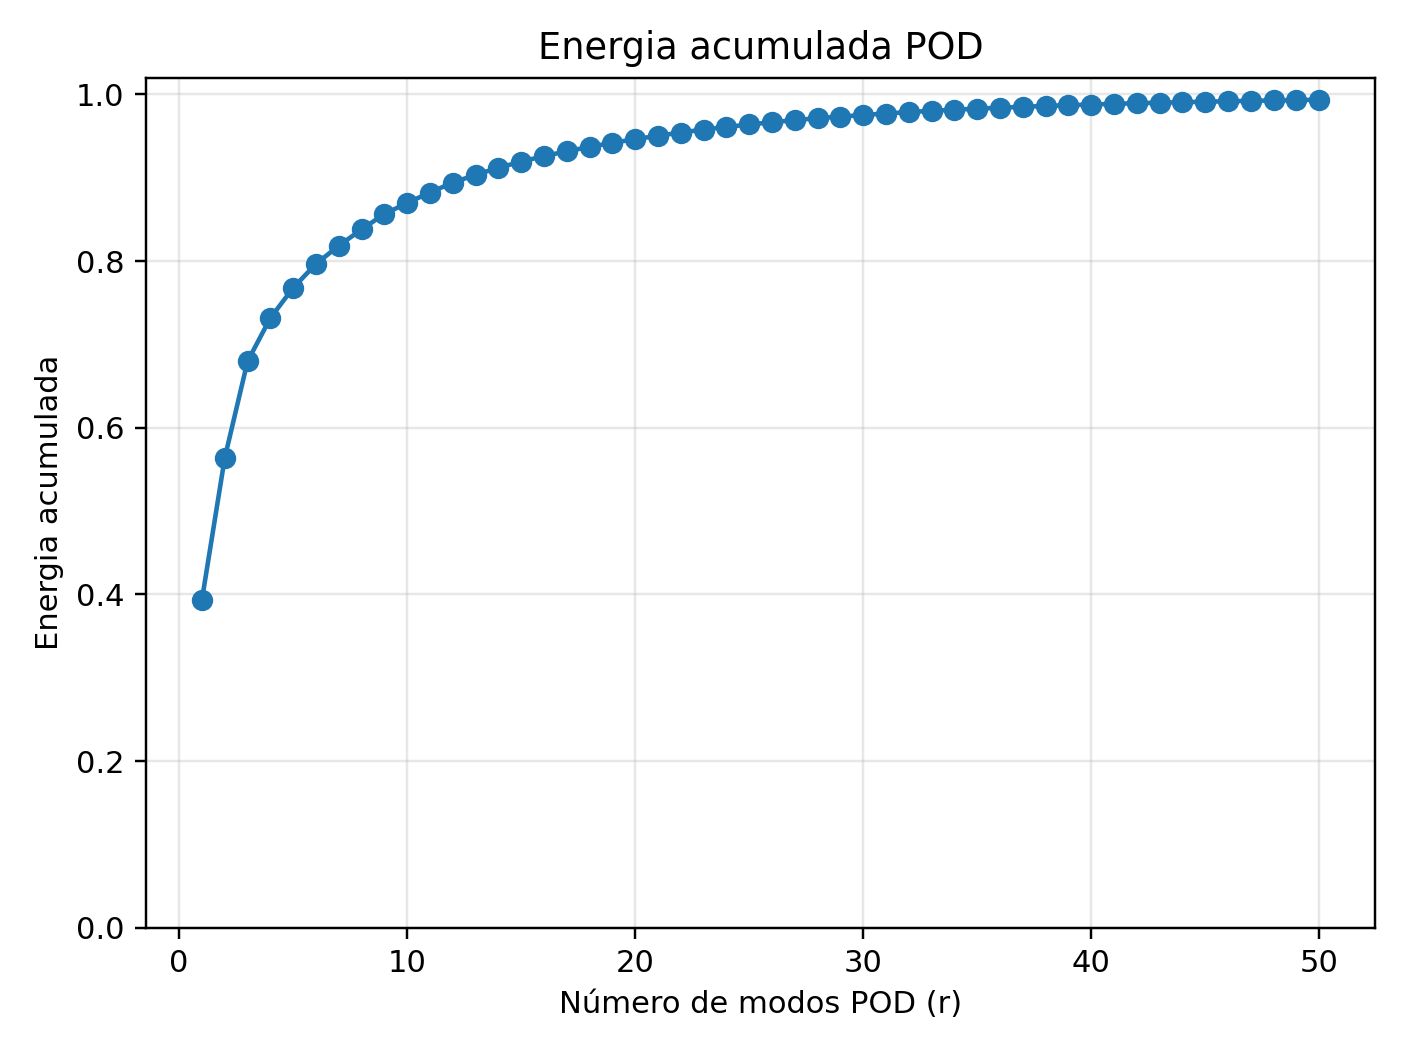
\includegraphics[width=\linewidth]{pod_energia.png}\caption{Energia acumulada.}\end{subfigure}
\begin{subfigure}{0.49\textwidth}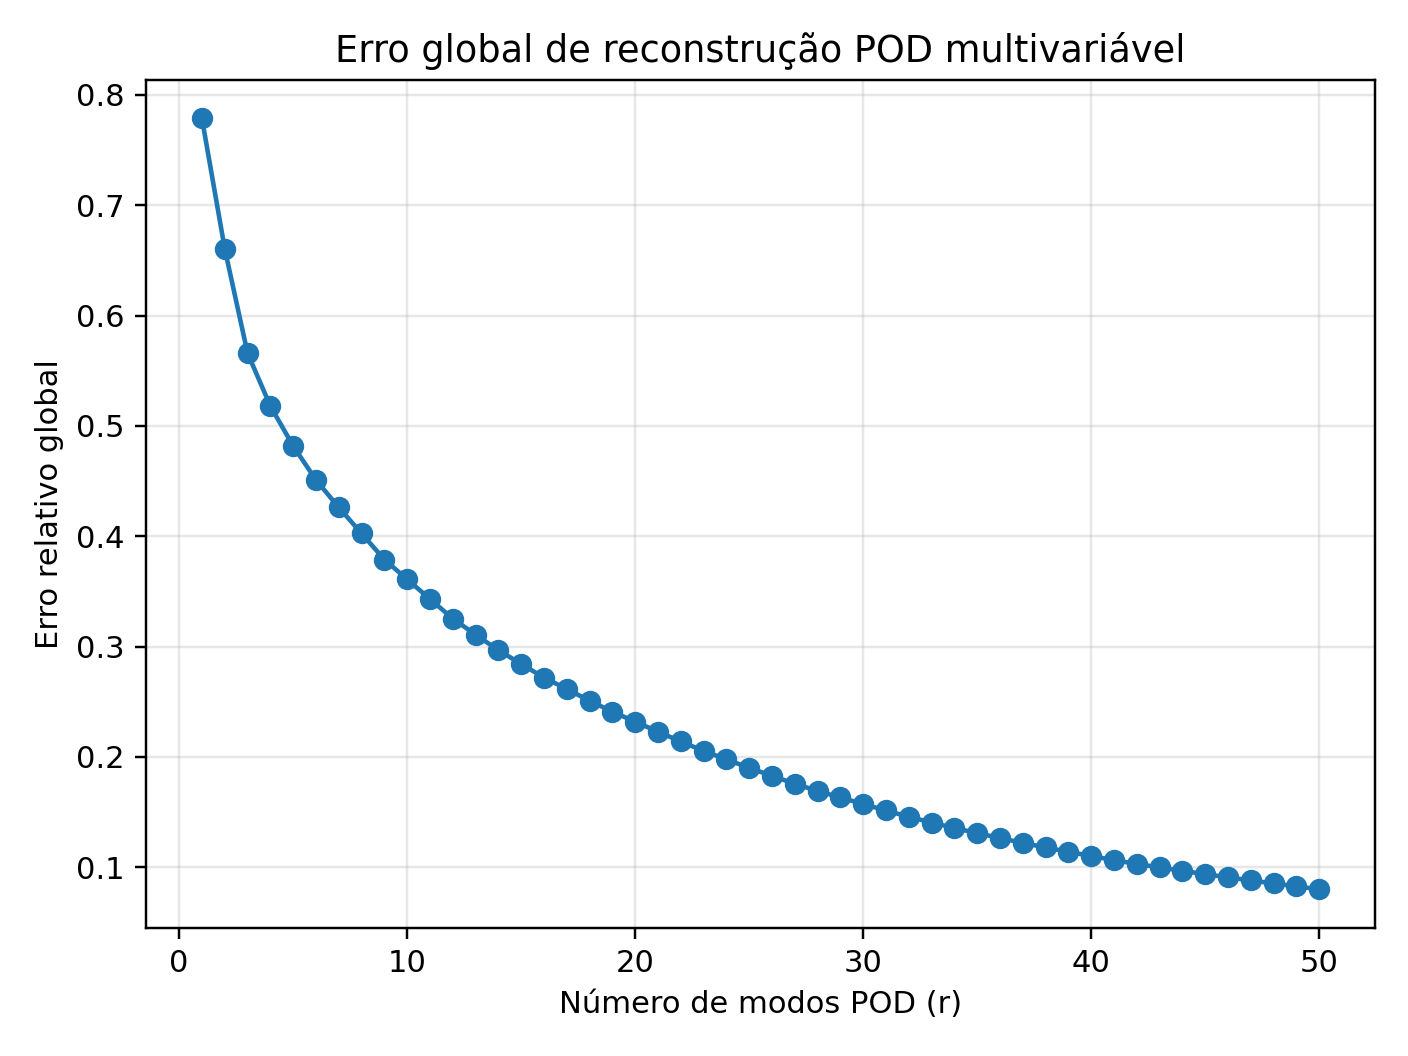
\includegraphics[width=\linewidth]{pod_erro_global.png}\caption{Erro global.}\end{subfigure}
\caption{Convergência da reconstrução POD com o número de modos.}
\label{fig:podconv}
\end{figure}

\begin{figure}[H]
\centering
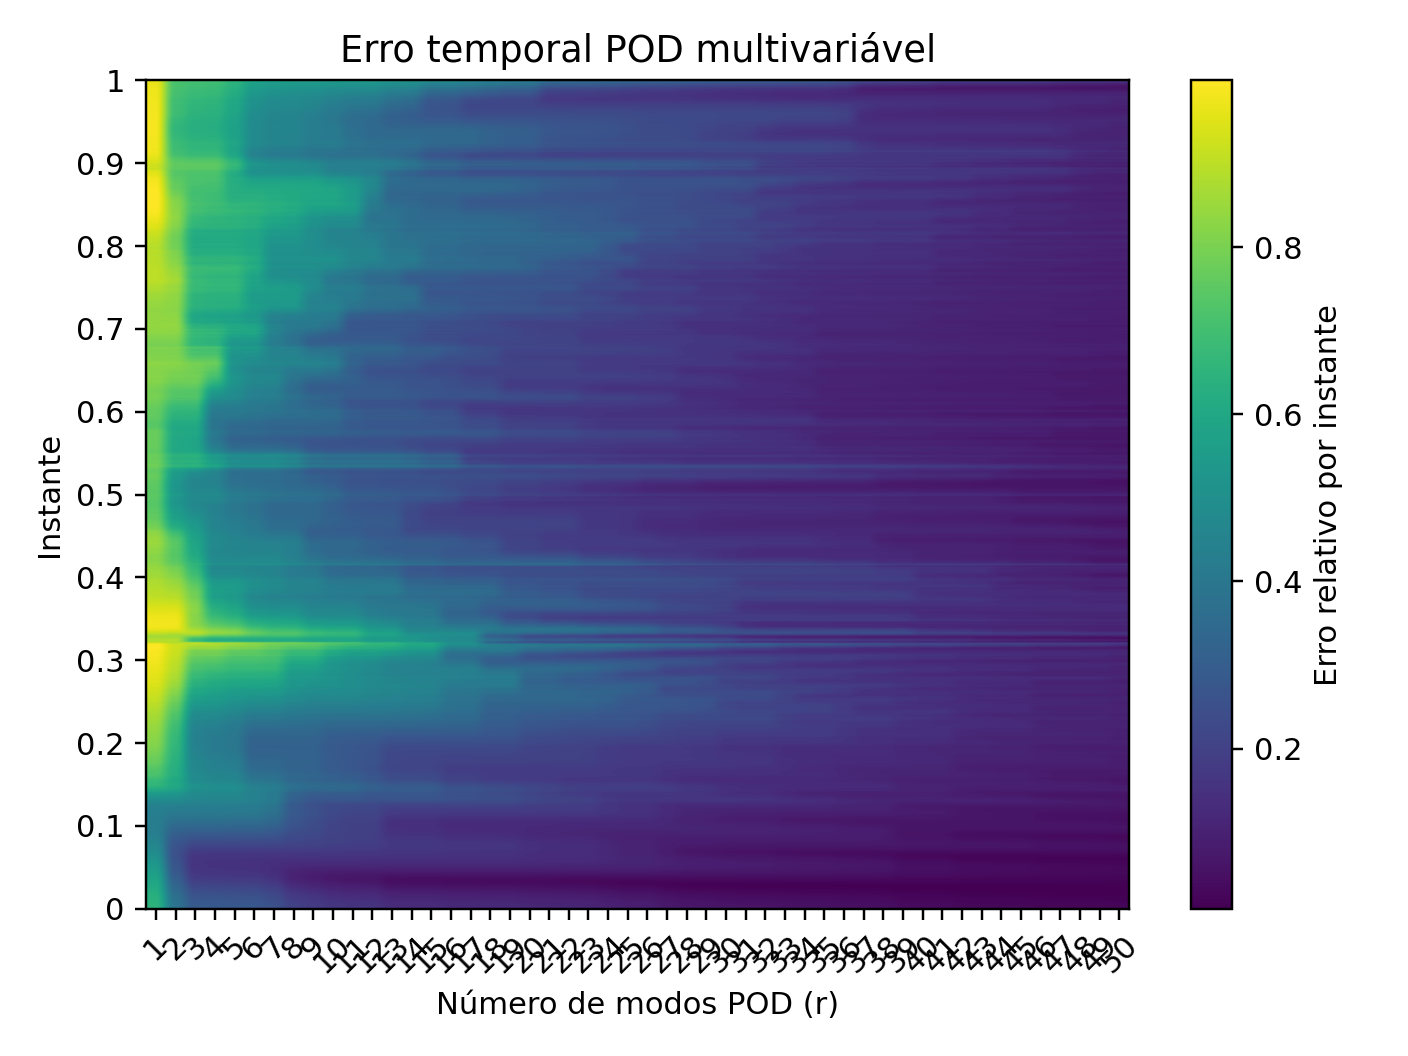
\includegraphics[width=0.92\textwidth]{pod_mapa_erro.png}
\caption{Distribuição temporal do erro POD em função do número de modos. A figura evidencia que instantes transientes exigem mais modos.}
\label{fig:podmap}
\end{figure}

\begin{figure}[H]
\centering
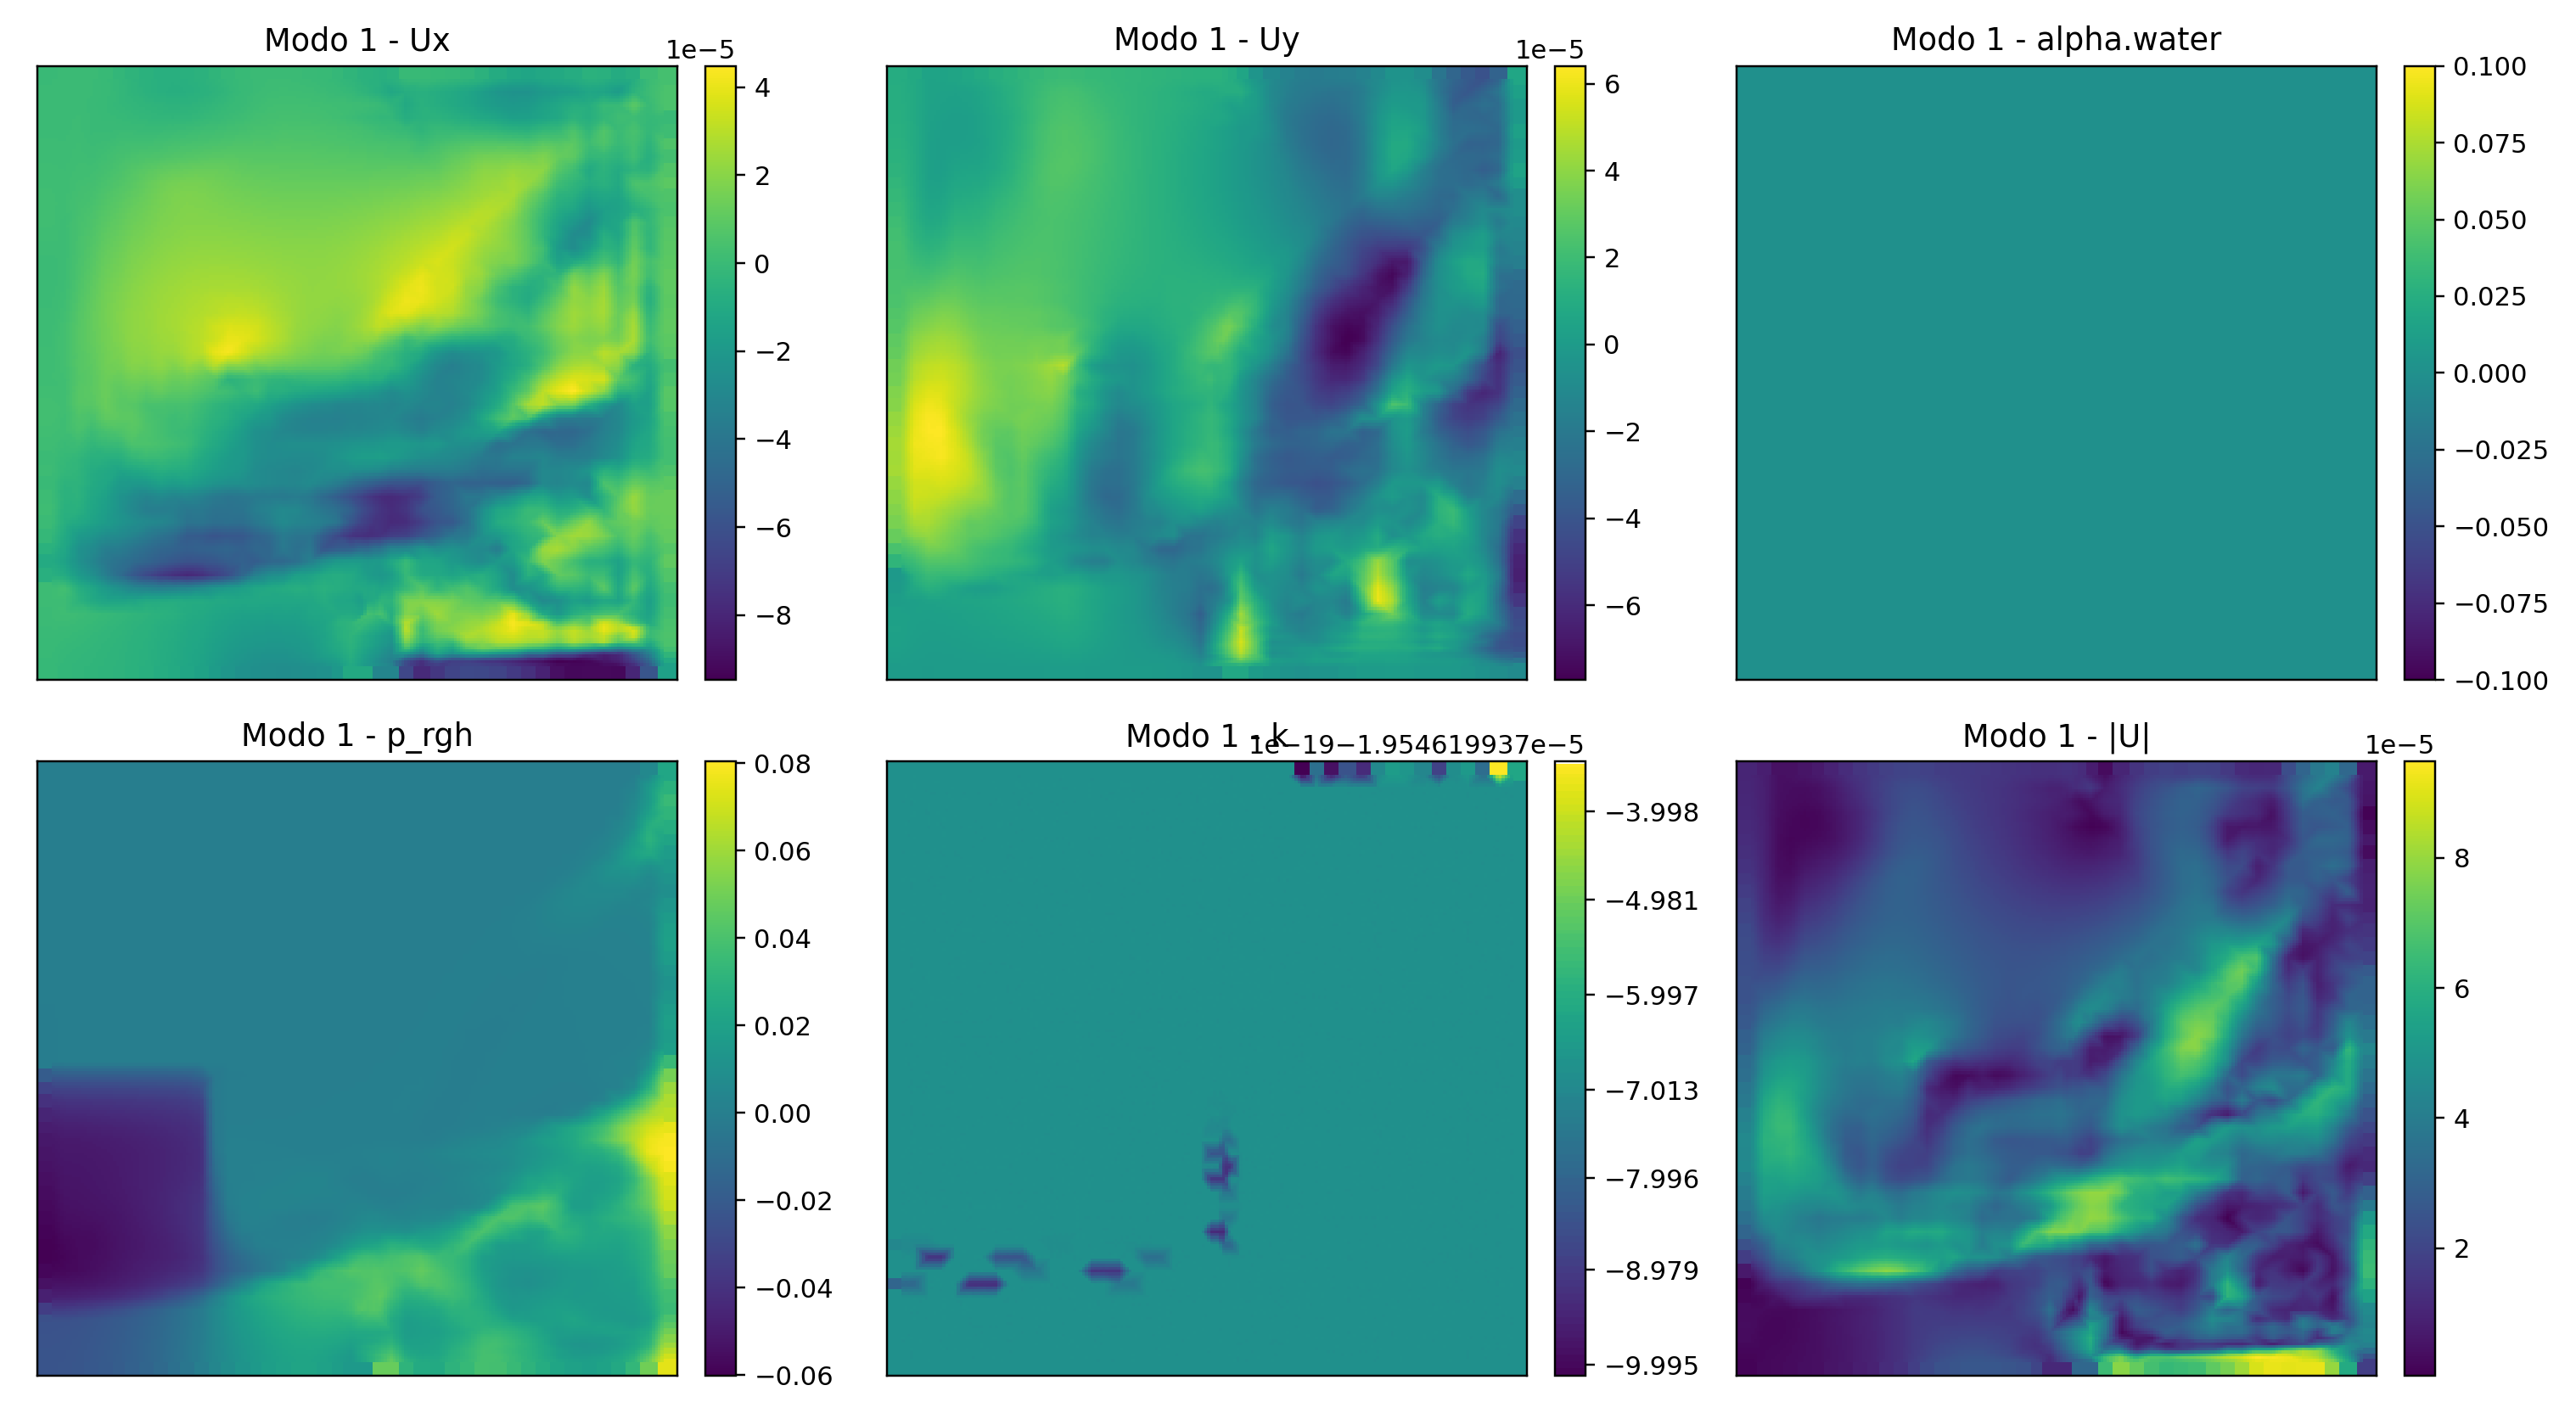
\includegraphics[width=0.95\textwidth]{pod_modo_01.png}
\caption{Estrutura espacial do primeiro modo POD para todos os canais armazenados. O canal $k$ aparece nulo devido à ausência desse campo no caso LES--WALE.}
\label{fig:podmodo1}
\end{figure}

\begin{figure}[H]
\centering
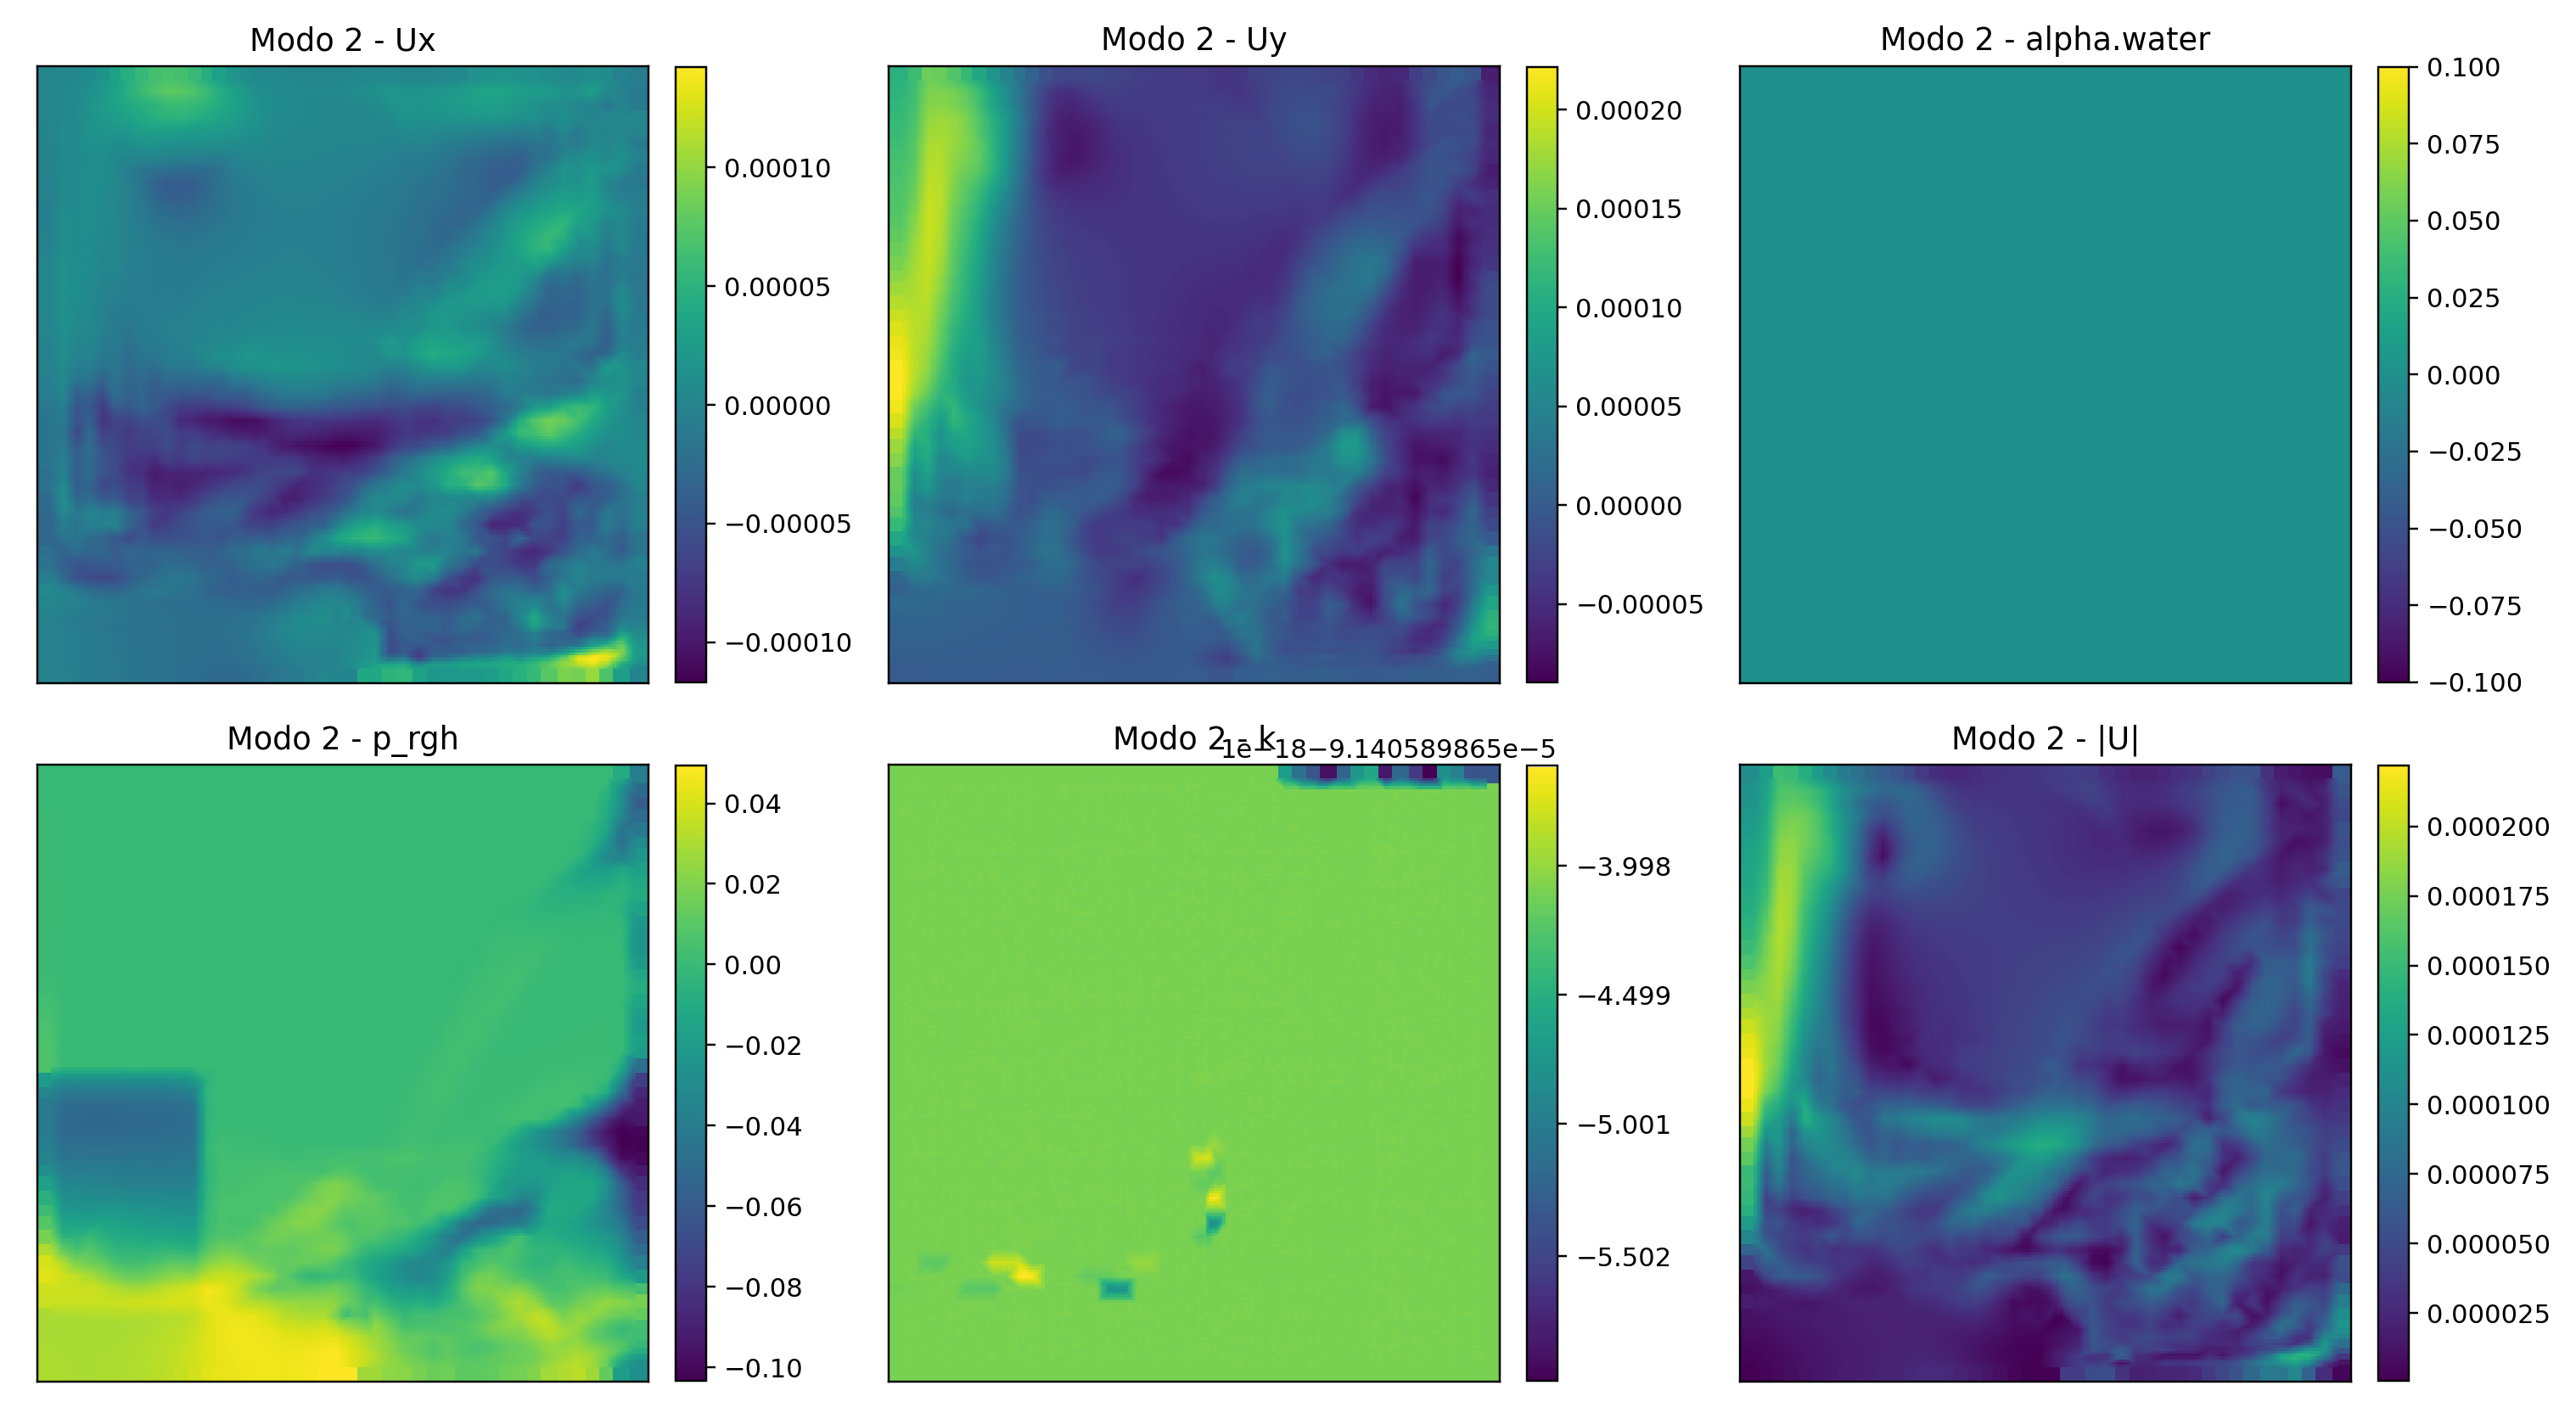
\includegraphics[width=0.95\textwidth]{pod_modo_02.png}
\caption{Estrutura espacial do segundo modo POD.}
\label{fig:podmodo2}
\end{figure}

\begin{figure}[H]
\centering
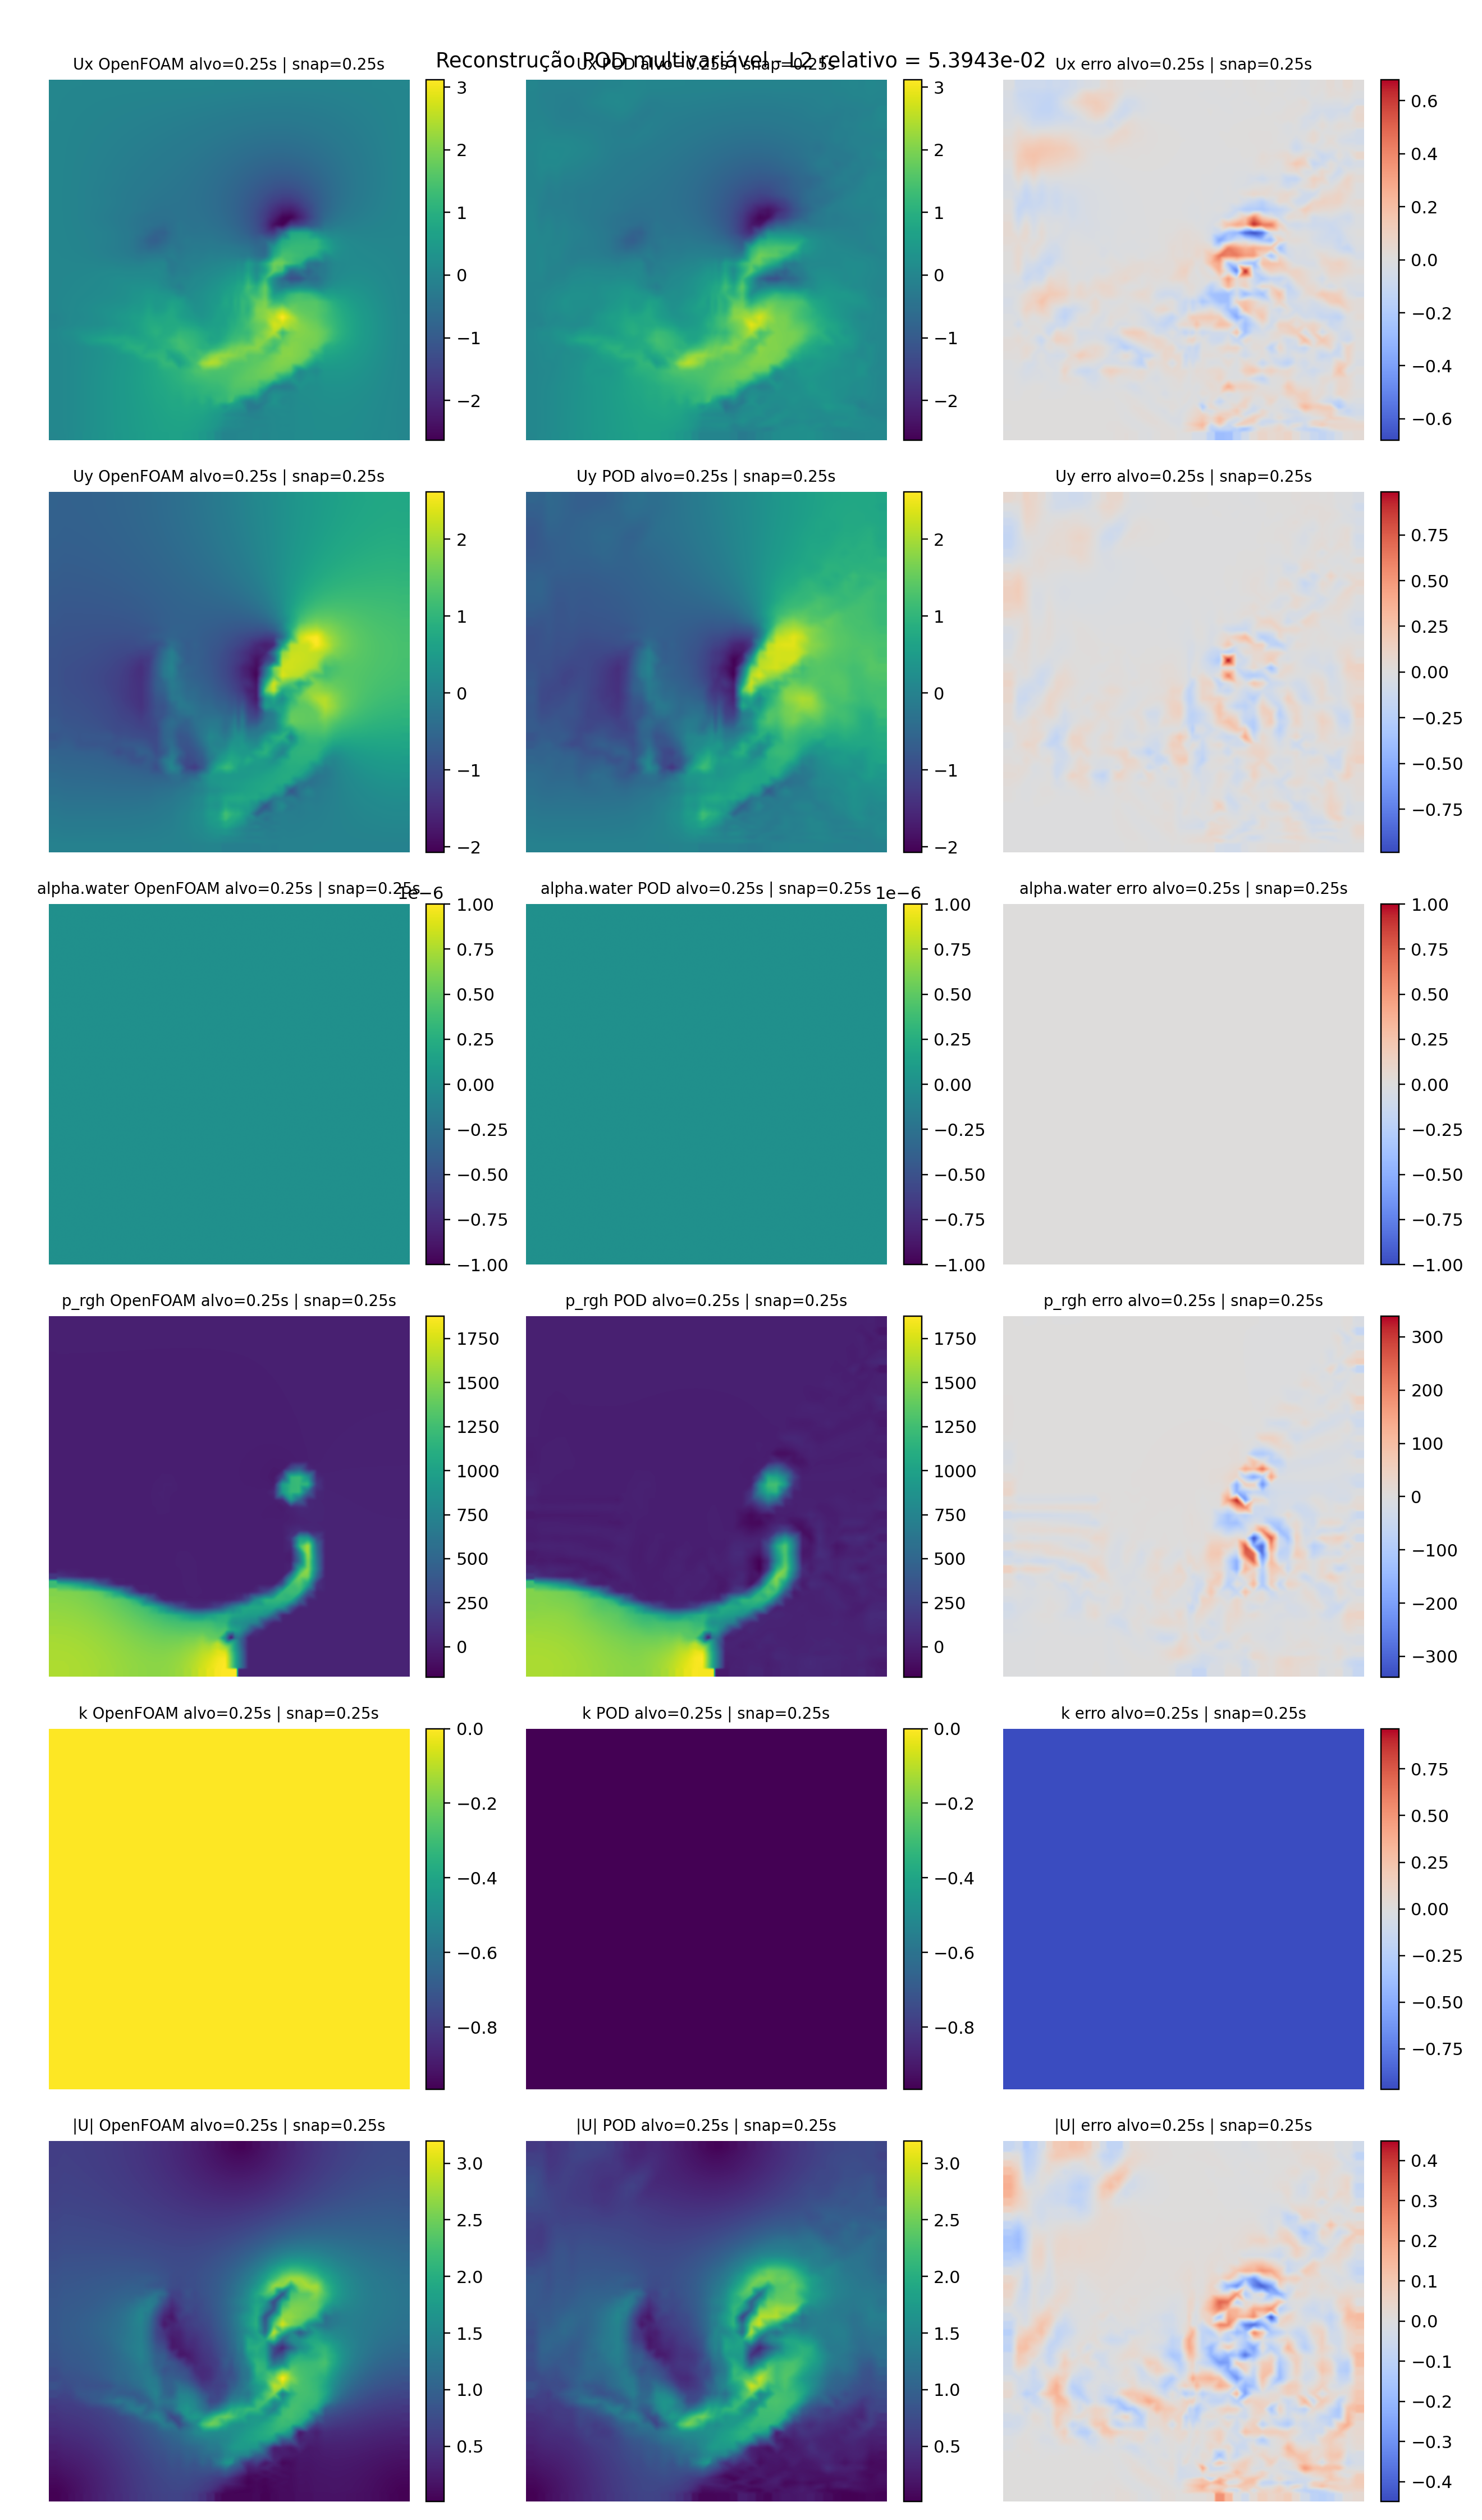
\includegraphics[height=0.80\textheight,keepaspectratio]{pod_t025.png}
\caption{Reconstrução POD multivariável isolada em $t=\SI{0.25}{s}$: referência OpenFOAM, reconstrução e erro.}
\label{fig:podt025}
\end{figure}

\begin{figure}[H]
\centering
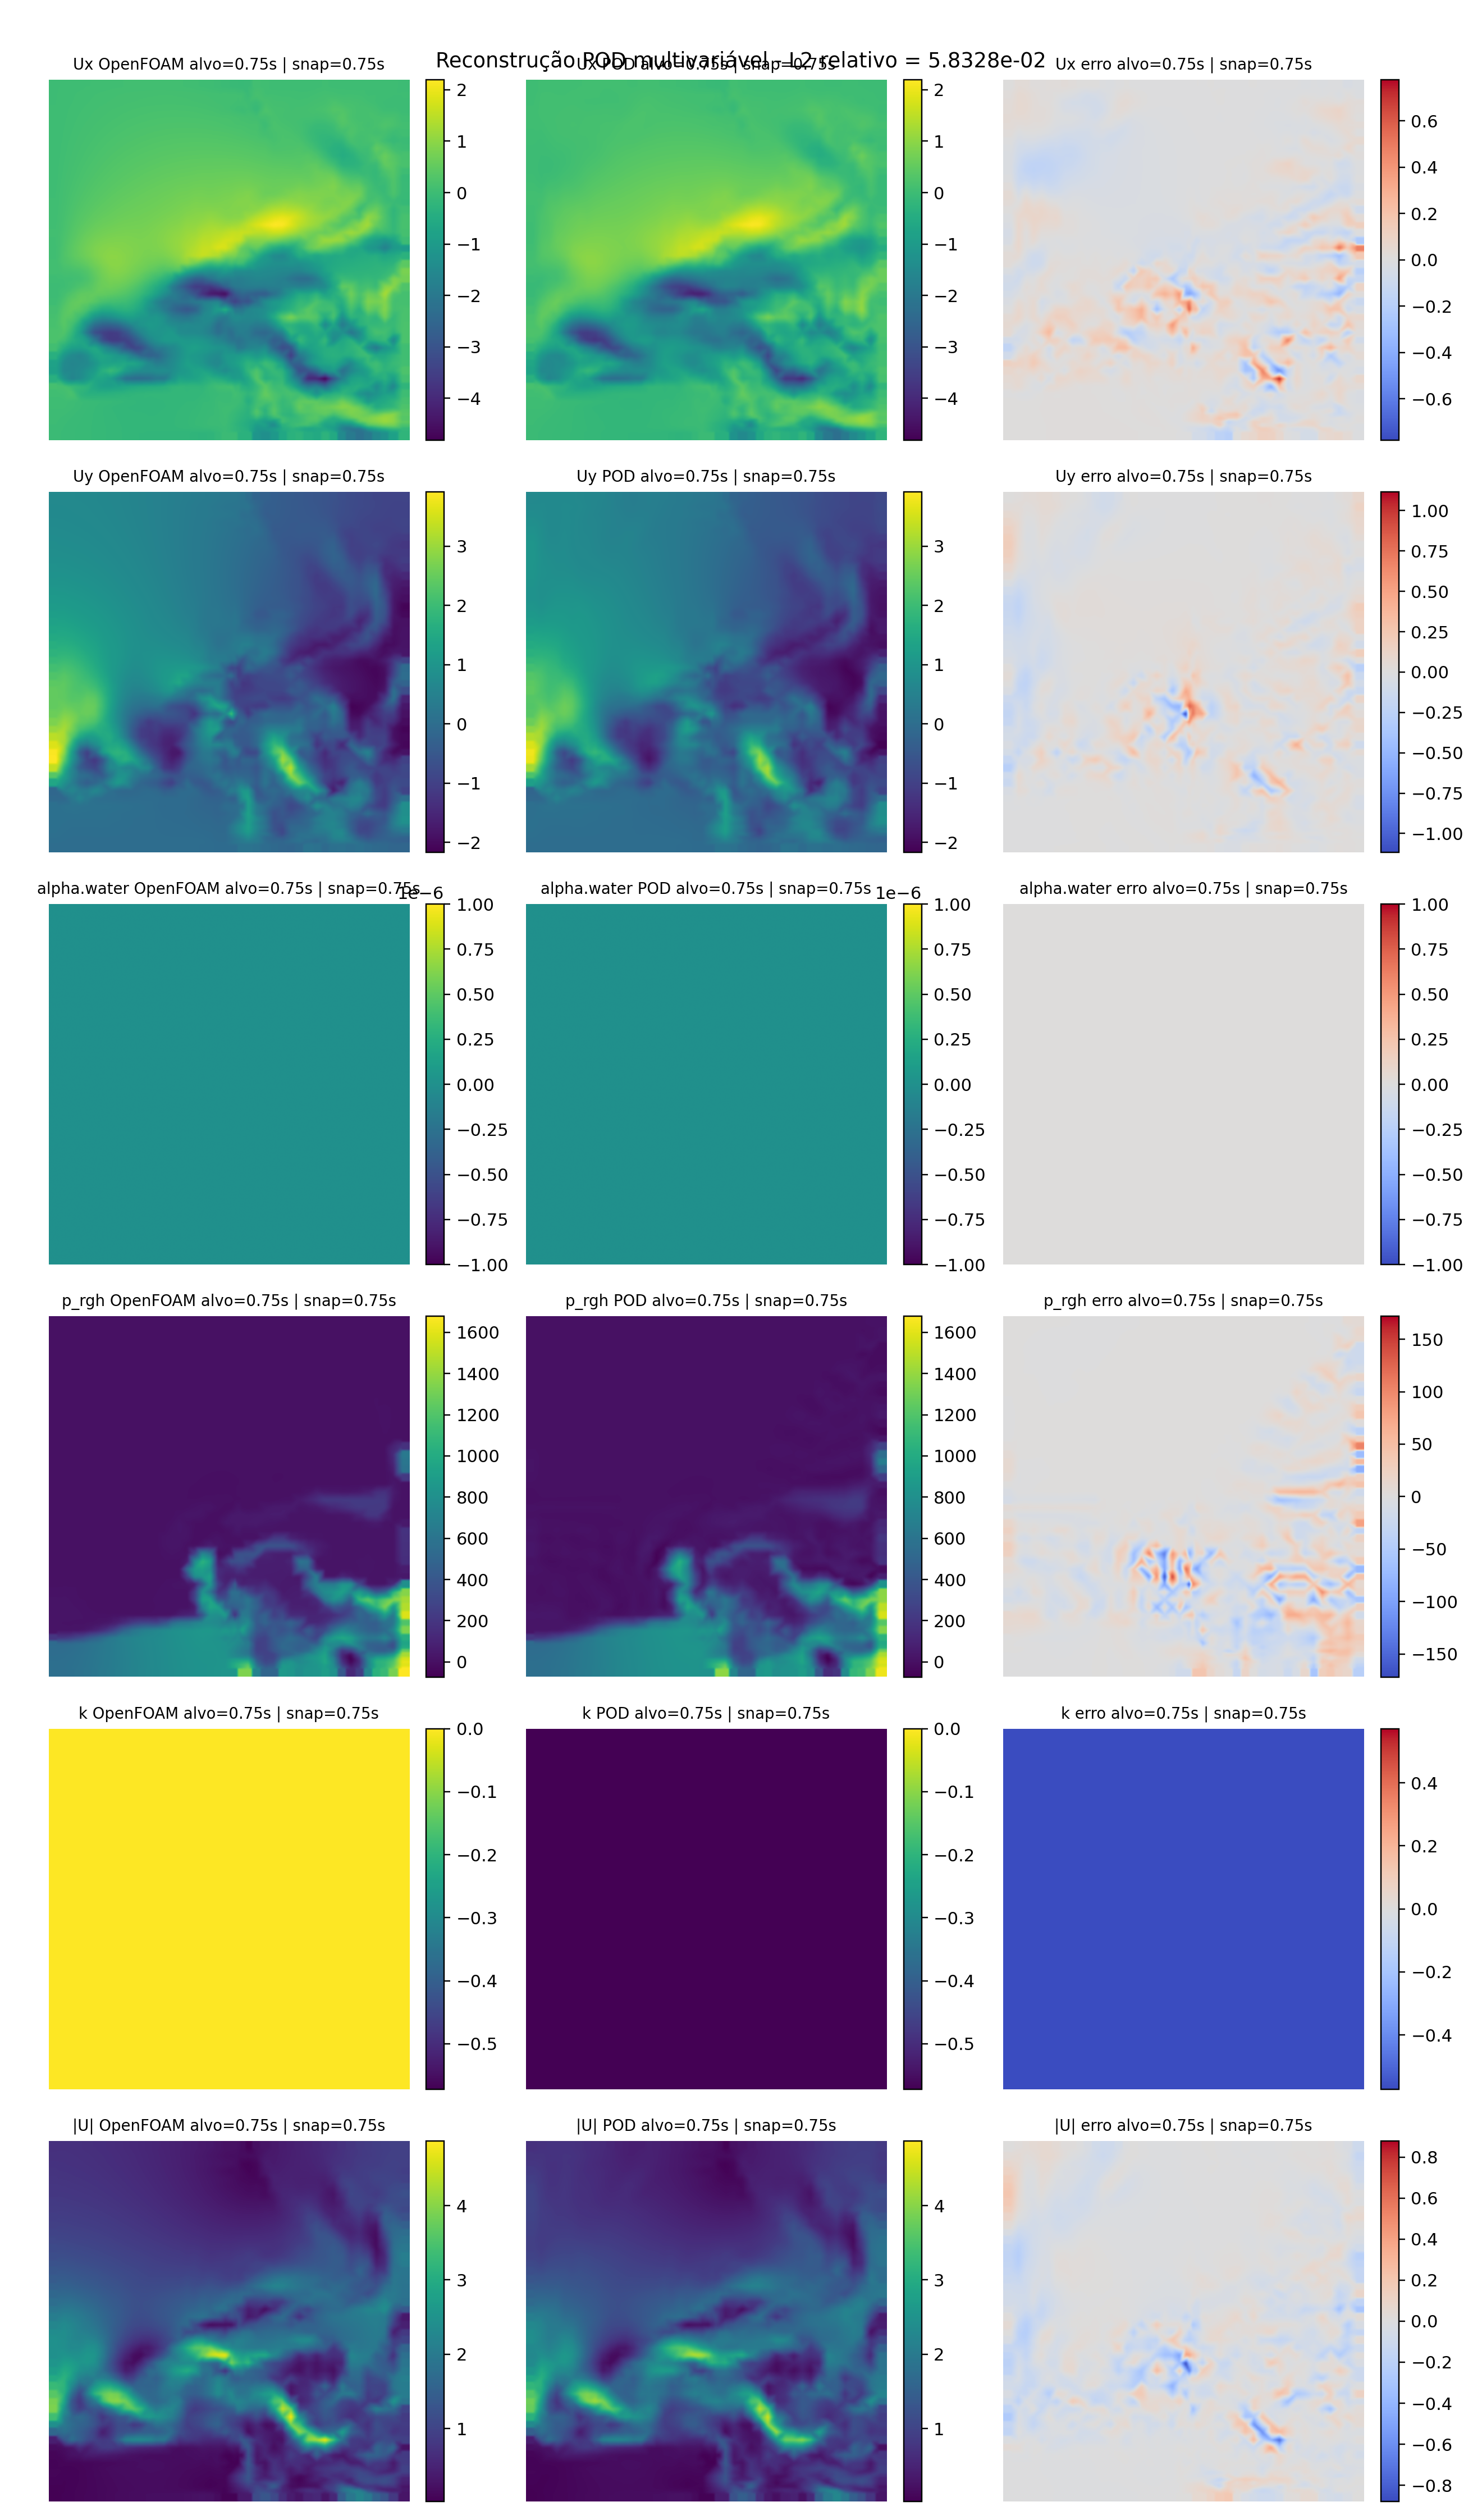
\includegraphics[height=0.80\textheight,keepaspectratio]{pod_t075.png}
\caption{Reconstrução POD multivariável isolada em $t=\SI{0.75}{s}$.}
\label{fig:podt075}
\end{figure}

\begin{figure}[H]
\centering
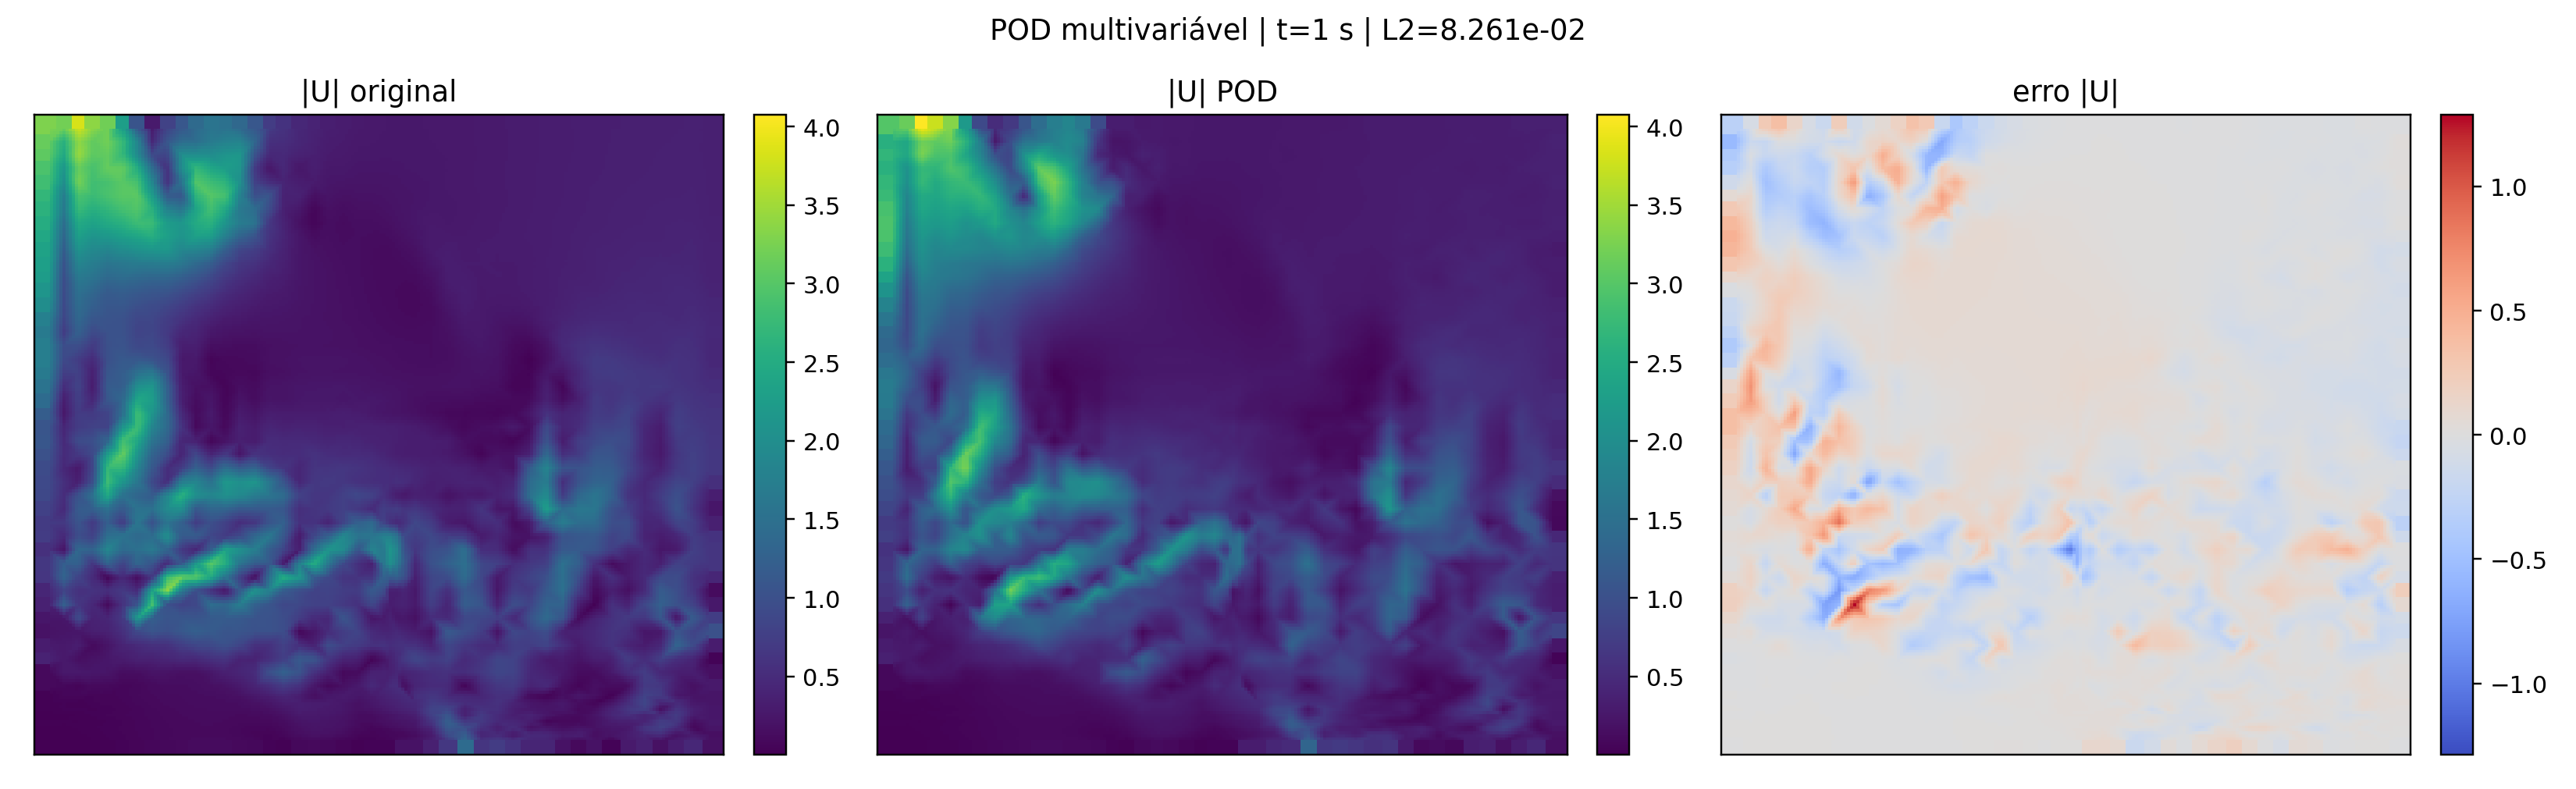
\includegraphics[width=0.86\textwidth]{pod_pior_U_t1.png}
\caption{Exemplo do maior erro POD salvo para a magnitude da velocidade, em $t=\SI{1}{s}$.}
\label{fig:podpior}
\end{figure}

\paragraph{Pontos positivos.} Há monotonicidade energia--erro, 99,36\% da energia com 50 modos e erro global de 8,00\%. A base é interpretável, ordenada por energia e não requer otimização não convexa.

\paragraph{Pontos negativos.} Com os oito modos usados no primeiro POD--SINDy, apenas 83,80\% da energia é preservada e o erro de projeção já é 40,25\%, antes de qualquer erro dinâmico. A POD representa apenas um subespaço linear; frentes móveis, impacto, quebra de interface e estruturas advectivas podem requerer muitos modos. Além disso, normalizar cada snapshot altera a ponderação física entre tempos e canais, e o canal $k$ nulo deve ser corrigido.

\section{Redução não linear por SAE}

\subsection{Arquitetura e correções}
O SAE aproxima $\widehat x=D(E(x))$, sendo $z=E(x)$ a coordenada latente e $D$ o decodificador. Em contraste com a POD, as ativações densas permitem uma variedade de redução não linear. Os dados OpenFOAM foram interpolados em grade $48\times48$ com cinco canais: $U_x$, $U_y$, $\alpha_{water}$, $p_{rgh}$ e \code{nut}. O vetor de entrada tem 11520 componentes.

\begin{table}[H]
\centering
\caption{Comparação das configurações SAE original e corrigida.}
\label{tab:saeparam}
\begin{tabularx}{\textwidth}{>{\bfseries}l X X}
\toprule
Parâmetro & Original & Corrigido\\
\midrule
Amostragem & \code{stride}=10: 101 snapshots & \code{stride}=1: 1001 snapshots\\
Treino/validação & 81/20, divisão temporal 80/20 & 801/200, divisão temporal 80/20\\
Encoder & 128--64--32 & 512--256--128\\
Dimensão latente & 8 & 32\\
Decoder & simétrico & simétrico\\
Taxa Adam & $5\times10^{-5}$ & $10^{-3}$\\
Épocas máximas & 150 & 300\\
Lote & 32 & 64\\
Batch normalization & ativa & desativada\\
Perda & Huber, $\delta=1$ & Huber, $\delta=1$\\
Regularização latente & $L_1=0$ & $L_1=0$\\
Normalização & por atributo, treino; corte $\pm4$ & piso $\sigma=10^{-3}$; corte $\pm6$\\
Callbacks & plateau 8, early stop 20 & plateau 15, early stop 40\\
\bottomrule
\end{tabularx}
\end{table}

O piso no desvio padrão foi introduzido porque regiões quase constantes de $\alpha_{water}$ e \code{nut} produziam z-scores excessivos fora do período de treino. A etiqueta \code{sae\_dense\_corrigido} evita sobrescrever diretamente os modelos antigos.

\subsection{Resultados do SAE}
\begin{table}[H]
\centering
\caption{Métricas de reconstrução armazenadas para os dois SAEs.}
\label{tab:saeres}
\begin{tabular}{lrrrrr}
\toprule
Modelo & melhor época & $\overline{L_2}^{tr}$ & $\overline{L_2}^{val}$ & $R^2_{tr}$ & $R^2_{val}$\\
\midrule
Original & 145 & 0,6412 & 0,8947 & 0,5853 & 0,1749\\
Corrigido & 52 & 0,0995 & 0,8142 & 0,9892 & 0,2631\\
\bottomrule
\end{tabular}
\end{table}

A correção reduziu o erro relativo médio de treino em aproximadamente 84,5\% e aumentou $R^2_{tr}$ para 0,989. Na validação temporal, a melhora foi bem menor: o erro médio caiu de 0,895 para 0,814 e $R^2$ subiu para apenas 0,263. Portanto, a capacidade de reconstrução do conjunto visto melhorou fortemente, mas a generalização para $t>\SI{0.8}{s}$ continua limitada.

\begin{figure}[H]
\centering
\begin{subfigure}{0.49\textwidth}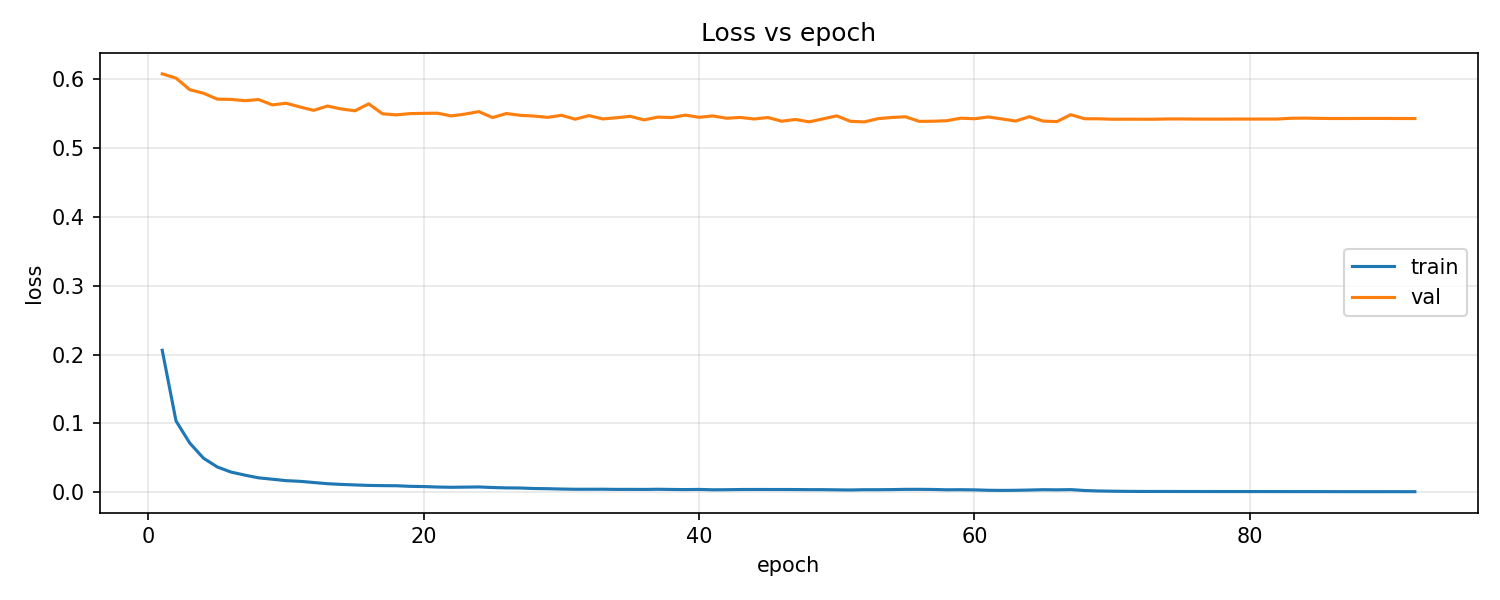
\includegraphics[width=\linewidth]{sae_loss.png}\caption{Perdas de treino e validação.}\end{subfigure}
\begin{subfigure}{0.49\textwidth}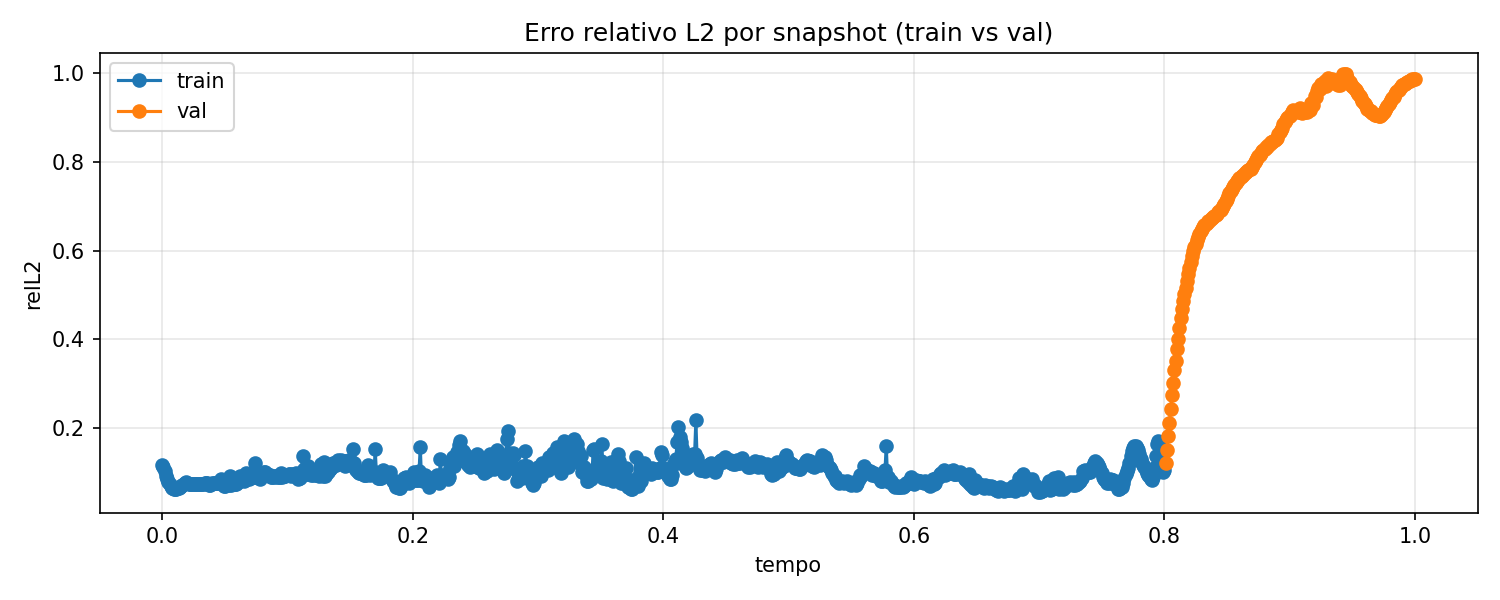
\includegraphics[width=\linewidth]{sae_relL2.png}\caption{Erro relativo por snapshot.}\end{subfigure}
\caption{Diagnóstico do SAE corrigido. A separação persistente entre treino e validação caracteriza mudança temporal e sobreajuste.}
\label{fig:saediag}
\end{figure}

\begin{figure}[H]
\centering
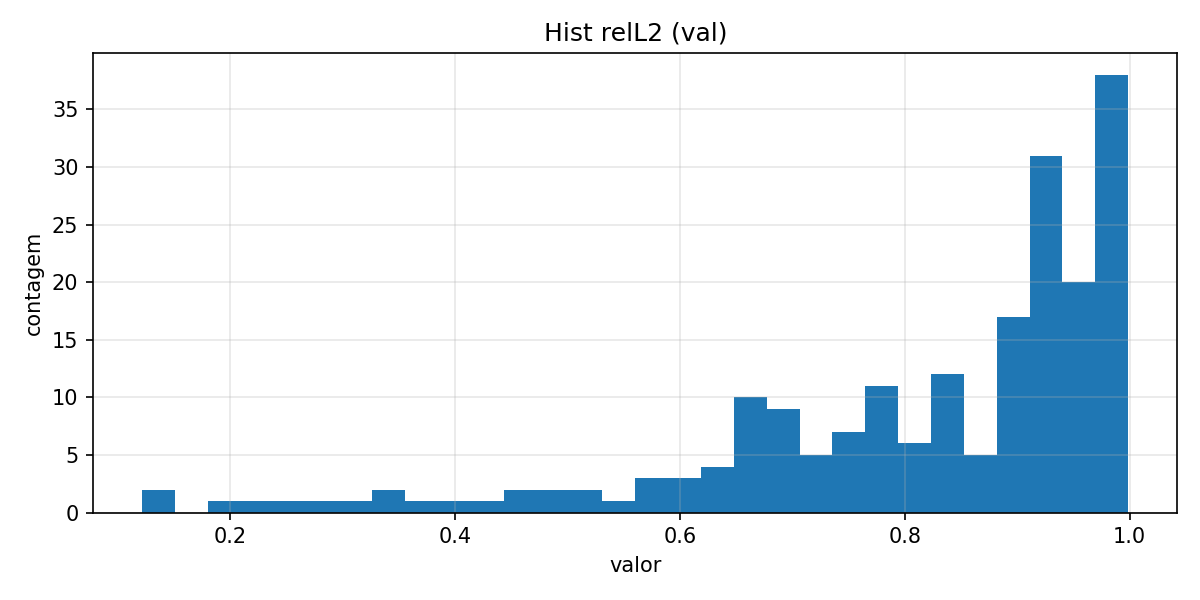
\includegraphics[width=0.62\textwidth]{sae_hist_val.png}
\caption{Distribuição do erro relativo do SAE no conjunto de validação.}
\label{fig:saehist}
\end{figure}

\begin{figure}[H]
\centering
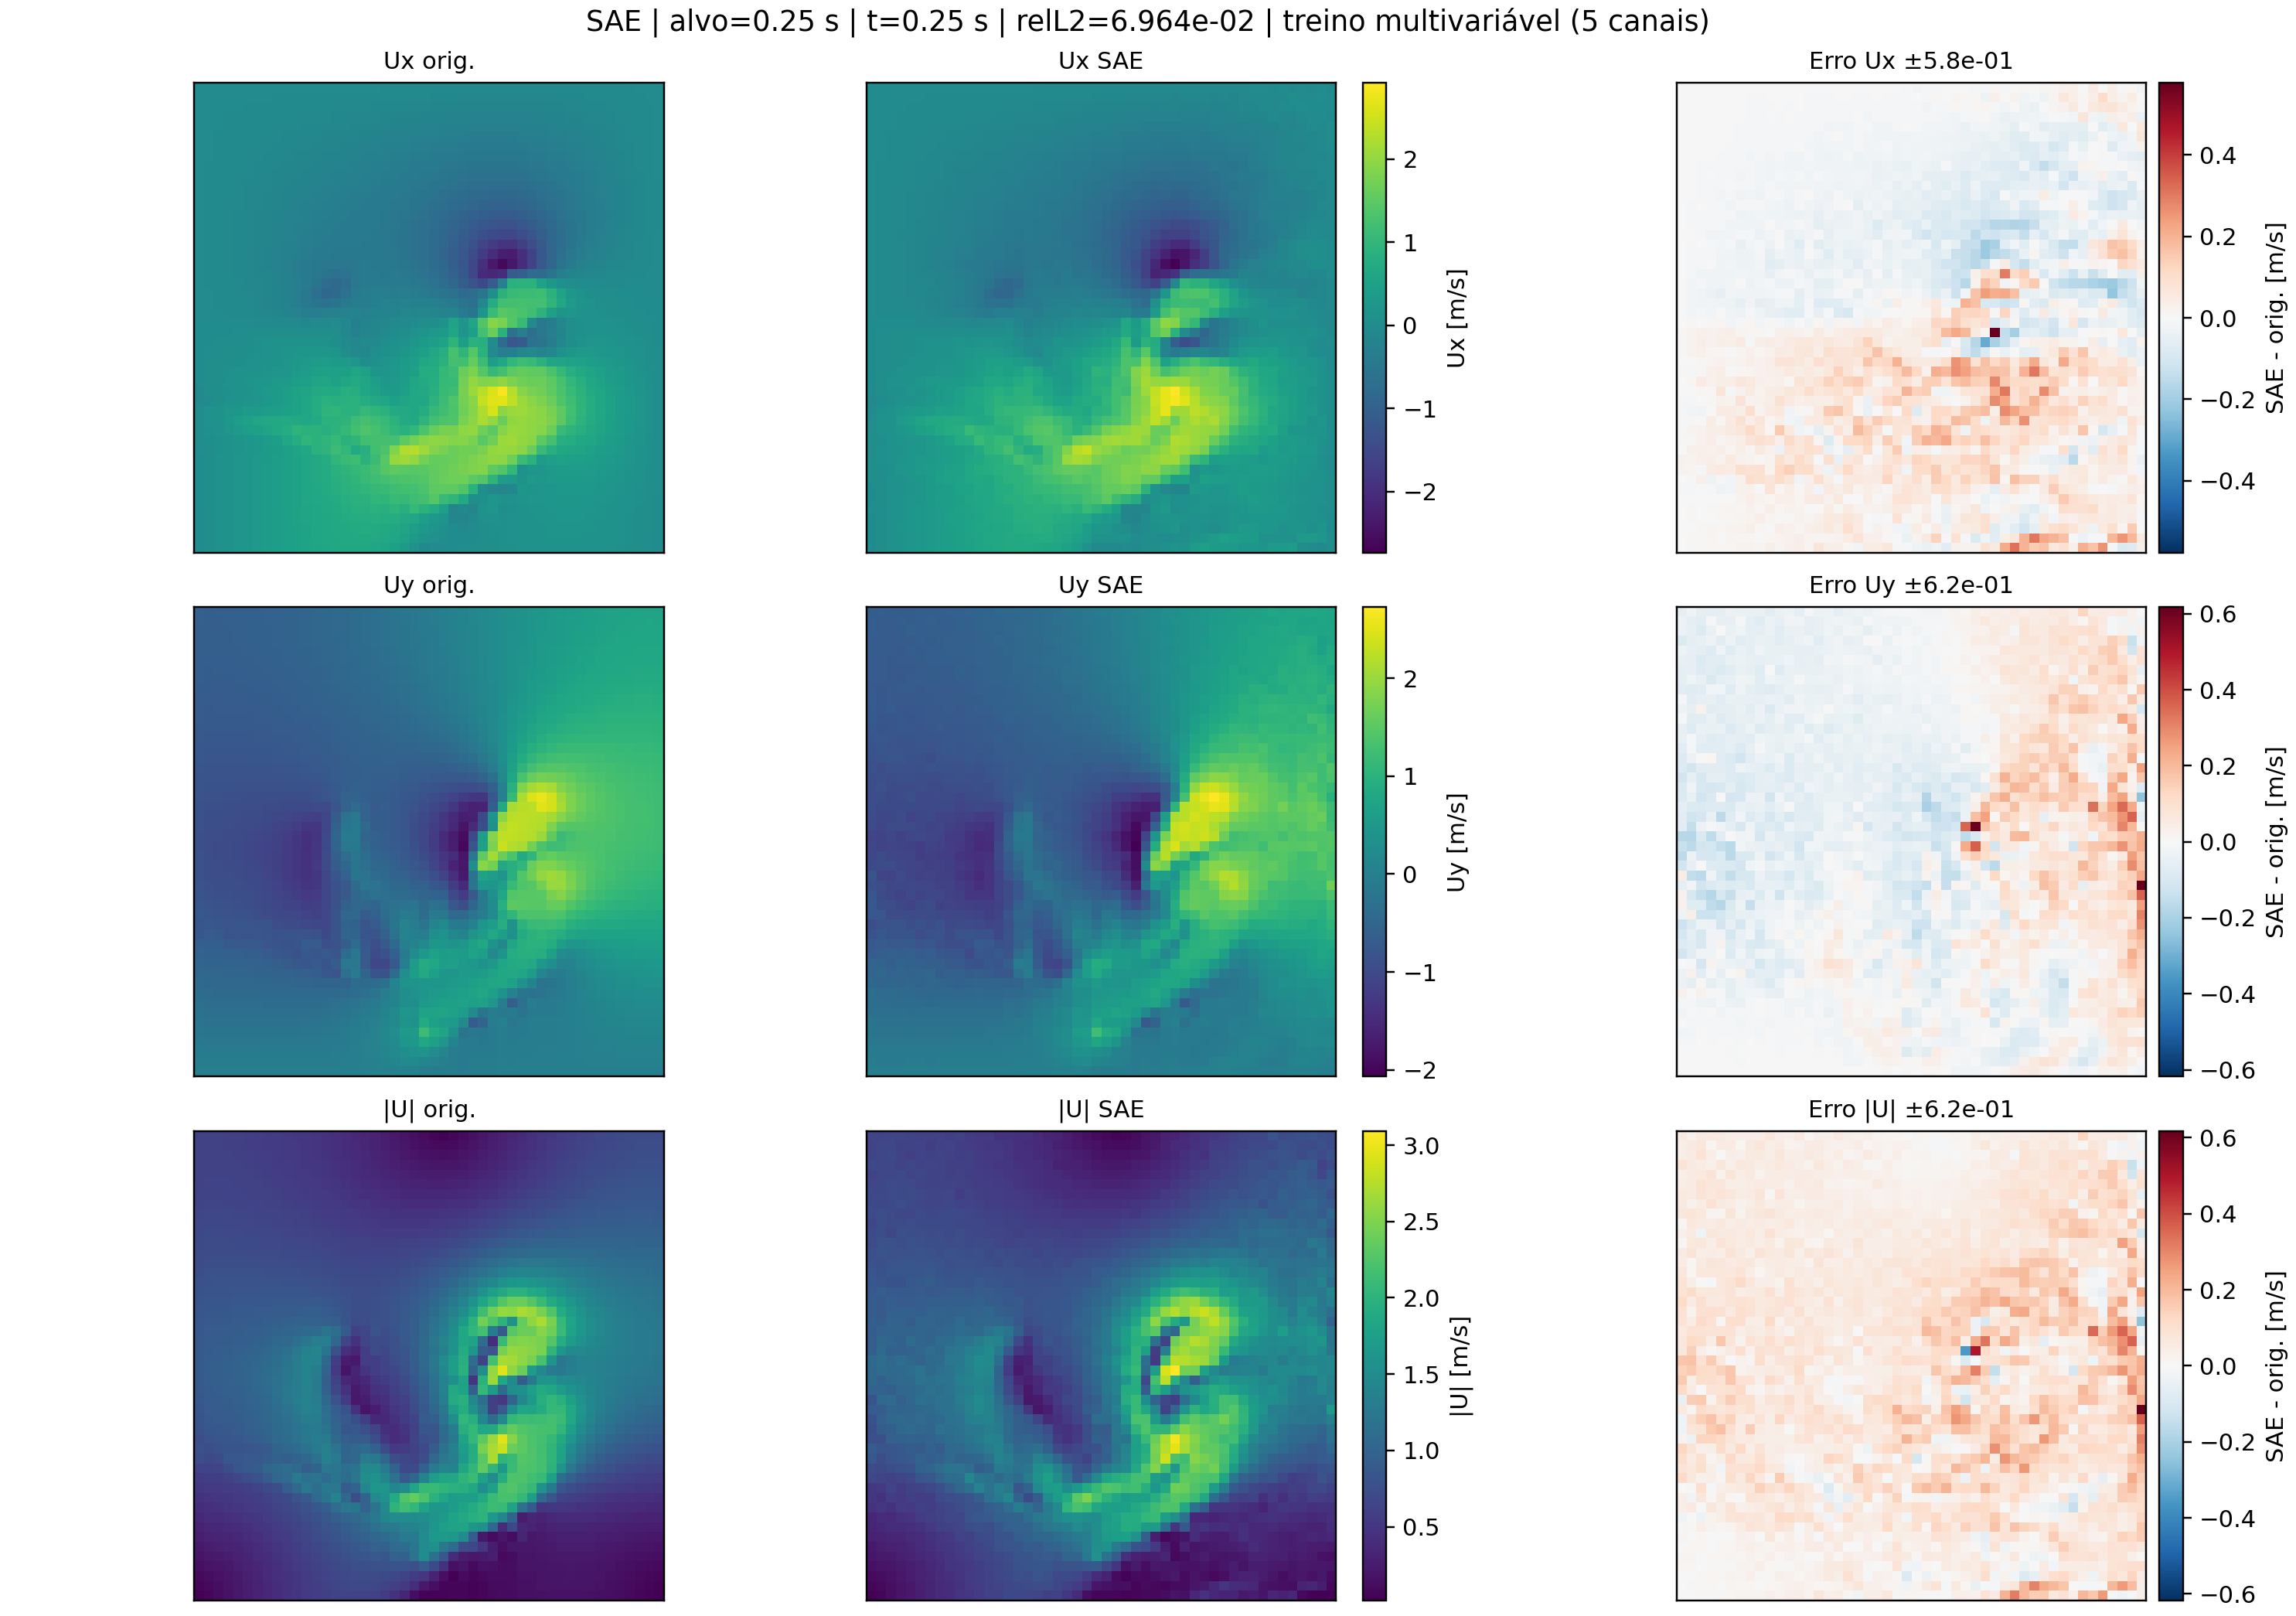
\includegraphics[width=0.92\textwidth]{sae_t025.png}
\caption{Reconstrução SAE isolada em $t=\SI{0.25}{s}$: original, reconstrução e erro para $U_x$, $U_y$ e $|U|$.}
\label{fig:saet025}
\end{figure}

\begin{figure}[H]
\centering
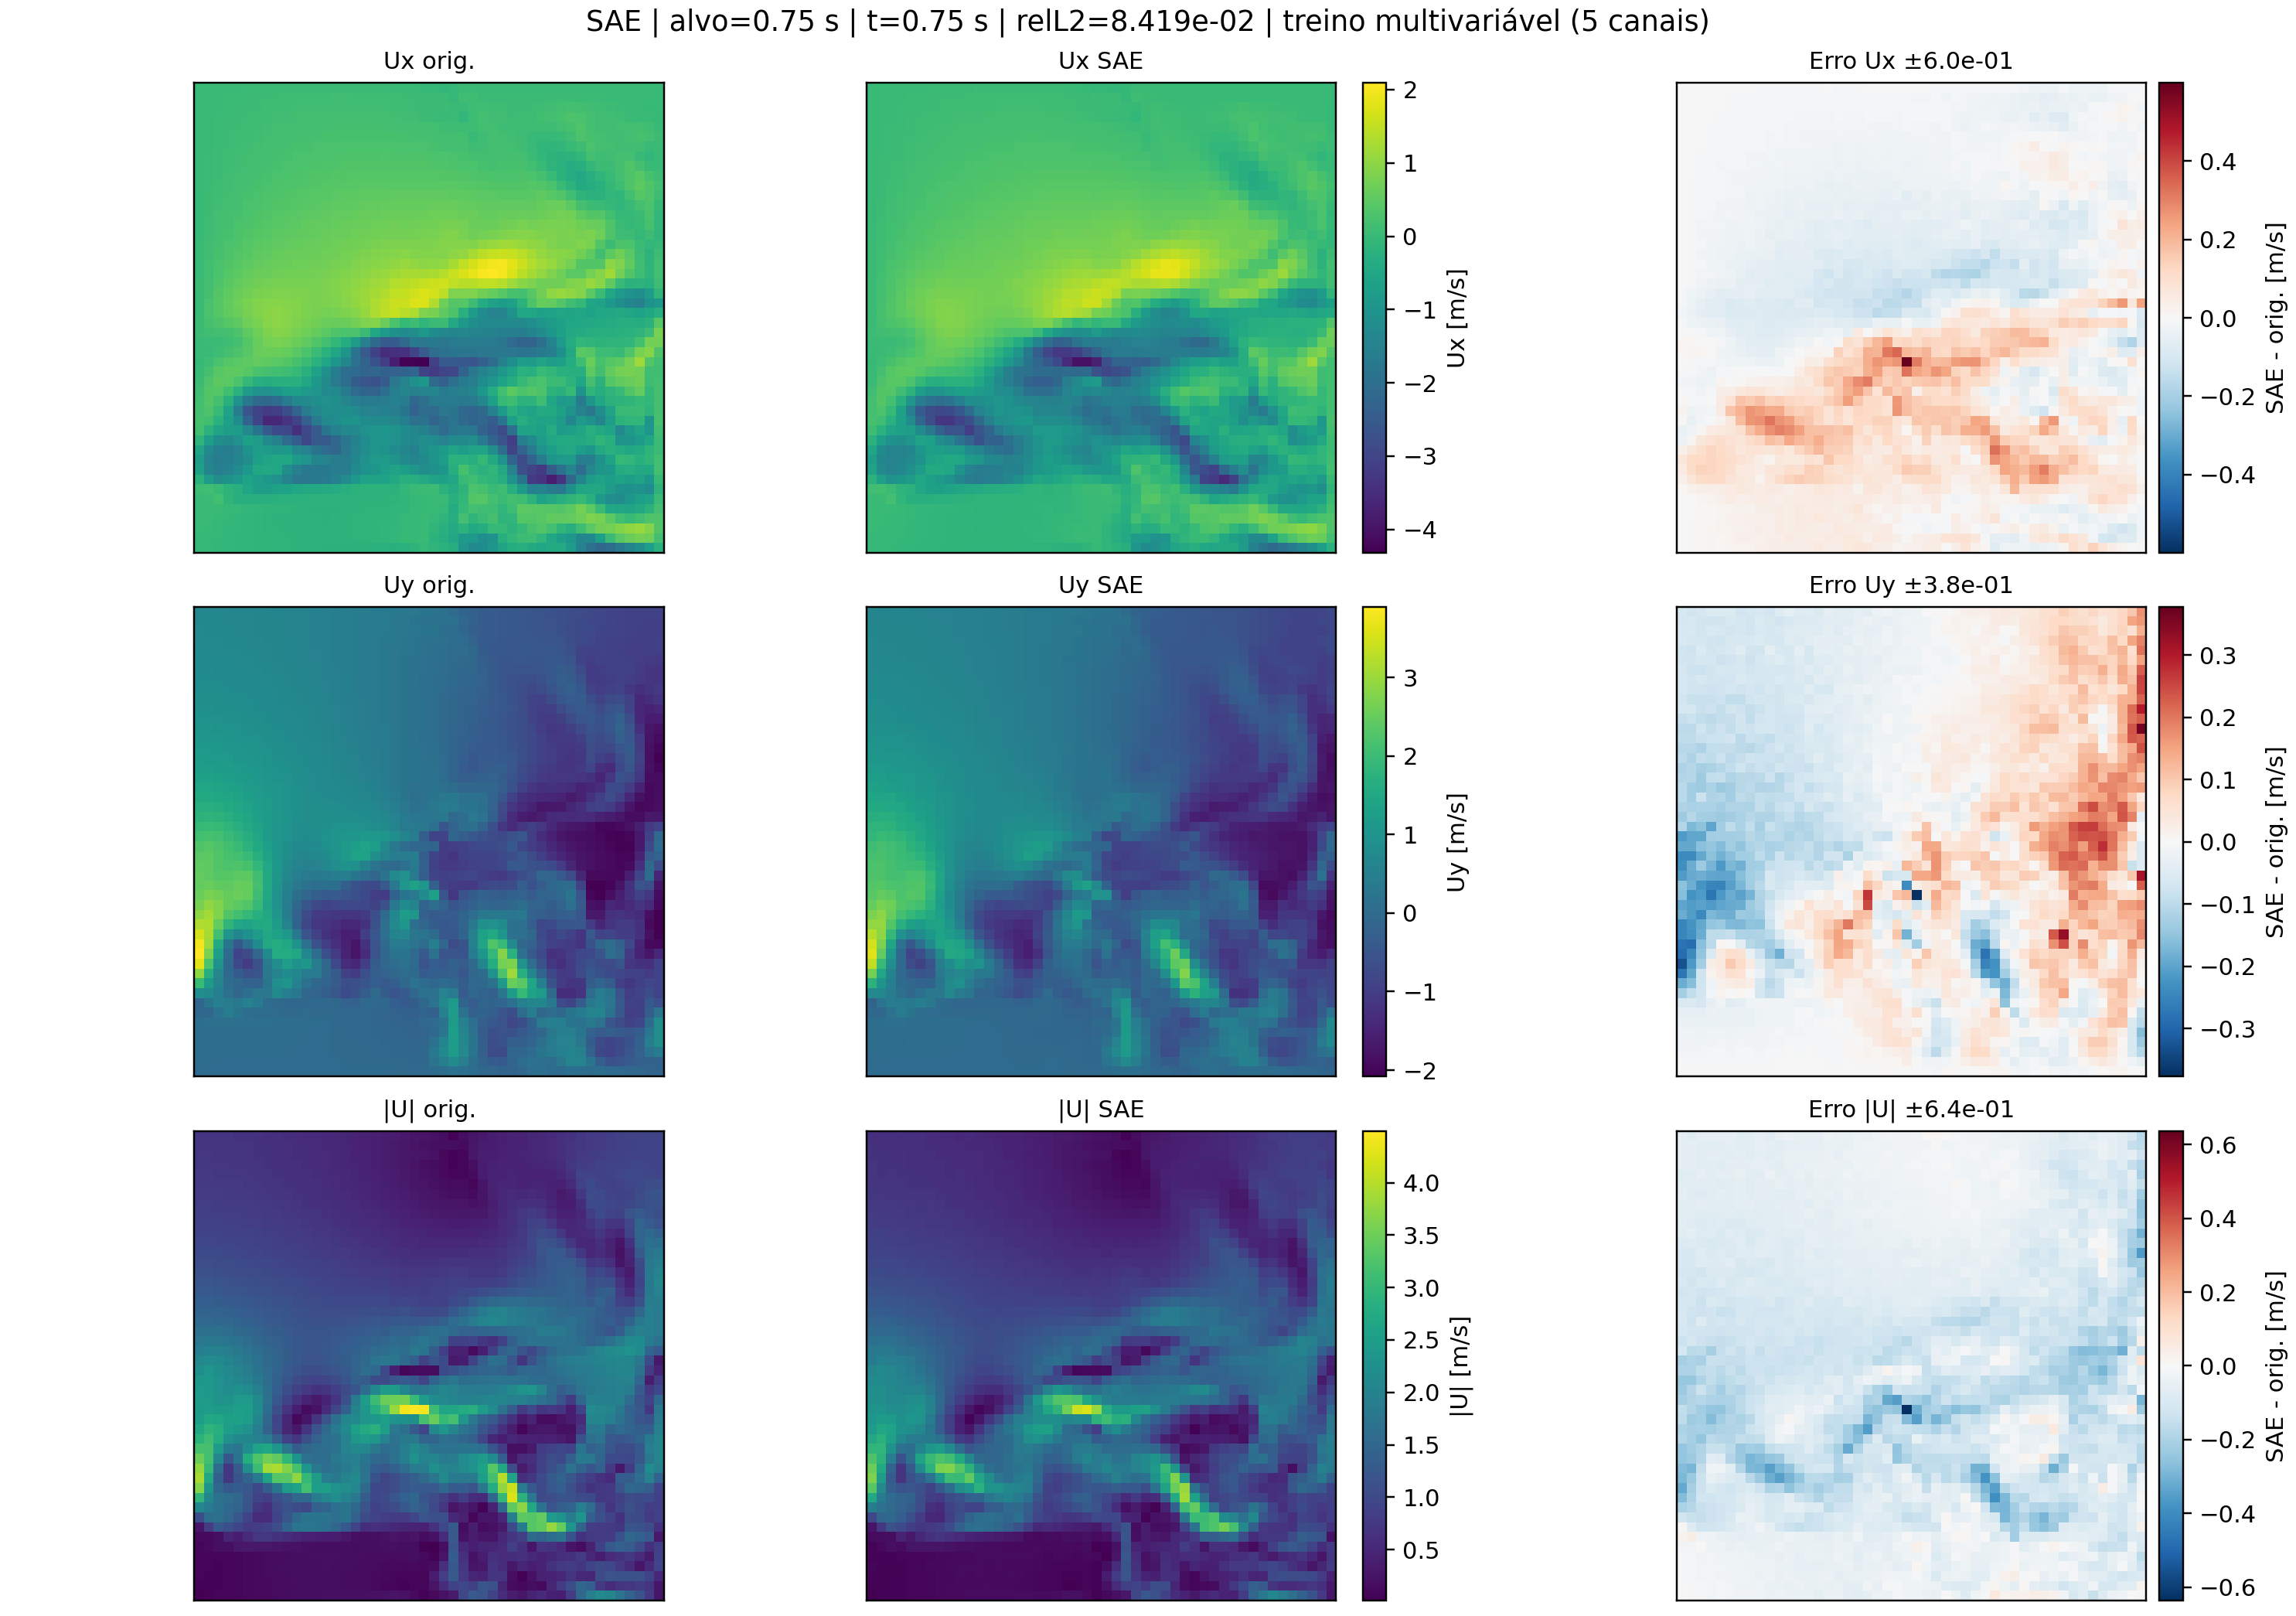
\includegraphics[width=0.92\textwidth]{sae_t075.png}
\caption{Reconstrução SAE isolada em $t=\SI{0.75}{s}$.}
\label{fig:saet075}
\end{figure}

\paragraph{Capacidade não linear.} O SAE pode curvar o espaço reduzido e, em princípio, representar interfaces móveis com menos coordenadas do que uma base linear. O excelente ajuste no treino é evidência de capacidade representacional, mas não prova que o latente tenha dinâmica simples ou autônoma. O grande \emph{gap} temporal mostra que a variedade aprendida no início não cobre adequadamente os estados finais. Um latente bom para reconstrução também não é necessariamente bom para diferenciação e integração por SINDy.

\section{Identificação dinâmica por SINDy}

SINDy busca um modelo esparso
\begin{equation}
 \dot q(t)=\Theta(q,t)\,\Xi,
\end{equation}
em que $q$ são coordenadas reduzidas, $\Theta$ contém funções candidatas e $\Xi$ deve ter poucos coeficientes não nulos. Ajustar $\dot q$ é um problema local; integrar o sistema desde a condição inicial é um teste global muito mais exigente. Erros pequenos nas derivadas podem se acumular e produzir grande erro de trajetória.

\subsection{POD como estabilizador do espaço latente segundo Lin, Xiao e Fang}
Lin, Xiao e Fang~\cite{lin2024} propõem a sequência SAE--POD--SINDy para descobrir equações de dinâmica de fluidos em uma variedade não linear reduzida. O SAE projeta os campos de alta dimensão no espaço latente $z(t)$; em seguida, a POD transforma esses códigos em coeficientes mais regulares,
\begin{equation}
 z(t)-\overline z \approx \Phi_r a(t),
 \qquad
 a(t)=\Phi_r^T\bigl(z(t)-\overline z\bigr),
\end{equation}
e o SINDy identifica $\dot a=\Theta(a)\Xi$. Segundo os autores, a aleatoriedade do treinamento do SAE pode produzir um espaço latente instável para regressão esparsa. A POD é introduzida para centralizar/ortogonalizar os códigos, suavizar a variedade reduzida e facilitar a aproximação polinomial e a descoberta pelo SINDy.

No artigo, transformações POD de mesma ordem do espaço latente são apresentadas como praticamente sem perda de energia, salvo arredondamento. Os testes de \emph{lock exchange} e escoamento ao redor de um e dois cilindros indicam maior correlação, menor RMSE e equações em alguns casos mais parcimoniosas após a POD. Os autores interpretam esses resultados como evidência de que padrões ou dinâmicas escondidos no espaço SAE tornam-se mais fáceis de identificar depois da transformação POD.

A implementação deste caso segue a mesma ideia geral, mas não é idêntica: os oito latentes do SAE antigo foram reduzidos para quatro modos POD, conservando 88,45\% da energia. Portanto, além de centralização e rotação, houve truncamento de 11,55\% da energia latente. Esse truncamento pode filtrar ruído e estabilizar o ajuste, mas também pode remover dinâmica relevante. A comparação deve, assim, considerar simultaneamente estabilidade, energia preservada e erro de integração livre.

A referência também ajuda a separar três operações diferentes:
\begin{itemize}
  \item SAE ou POD isolados apenas constroem coordenadas e reconstroem snapshots: são modelos de representação;
  \item SINDy introduz a lei temporal e transforma a representação em um modelo dinâmico;
  \item POD após SAE não cria a dinâmica; ela condiciona o espaço em que o SINDy procura essa dinâmica.
\end{itemize}

Logo, uma queda no erro de reconstrução ou no erro das derivadas não é suficiente para demonstrar captura dinâmica. Neste relatório, a integração livre continua sendo o teste mais rigoroso de que as equações identificadas reproduzem a evolução sem consultar os estados de referência.

\subsection{SINDy diretamente nas coordenadas POD}
O caso principal usou oito coeficientes POD, biblioteca polinomial de ordem 2 sem senos, Lasso e varredura de $\alpha\in\{10^{-4},3\cdot10^{-4},10^{-3},3\cdot10^{-3},10^{-2},3\cdot10^{-2},10^{-1}\}$. Com oito estados, a biblioteca possui 45 termos. Foi escolhido $\alpha=10^{-4}$.

\begin{table}[H]
\centering
\caption{Resultados do POD--SINDy salvo.}
\label{tab:podsindy}
\begin{tabularx}{\textwidth}{>{\bfseries}l X}
\toprule
Item & Resultado\\
\midrule
Snapshots / $\Delta t$ & 1001 / \SI{0.001}{s}\\
Estados POD & 8; energia capturada 0,8380\\
Biblioteca & ordem 2, sem seno; 45 termos por equação\\
Regressão & Lasso, $\alpha=10^{-4}$\\
Coeficientes não nulos & 149 de 360 possíveis\\
Erro relativo das derivadas & 0,4936\\
Erro relativo da trajetória livre & 1,6518\\
Integração & \code{solve\_ivp}\\
\bottomrule
\end{tabularx}
\end{table}

\subsubsection*{Equações descobertas: POD--SINDy}
As oito equações abaixo são exatamente as armazenadas em \code{pod\_sindy/equations.txt}. As variáveis $a_1,\ldots,a_8$ são os coeficientes dos oito primeiros modos POD. A grande quantidade de termos cruzados quadráticos evidencia que, mesmo em coordenadas POD lineares, a dinâmica identificada é não linear.
\lstinputlisting[style=sindyeq,caption={Sistema completo identificado pelo POD--SINDy.},label={lst:eqpodsindy}]{equacoes_pod_sindy.txt}

\begin{figure}[H]
\centering
\begin{subfigure}{0.49\textwidth}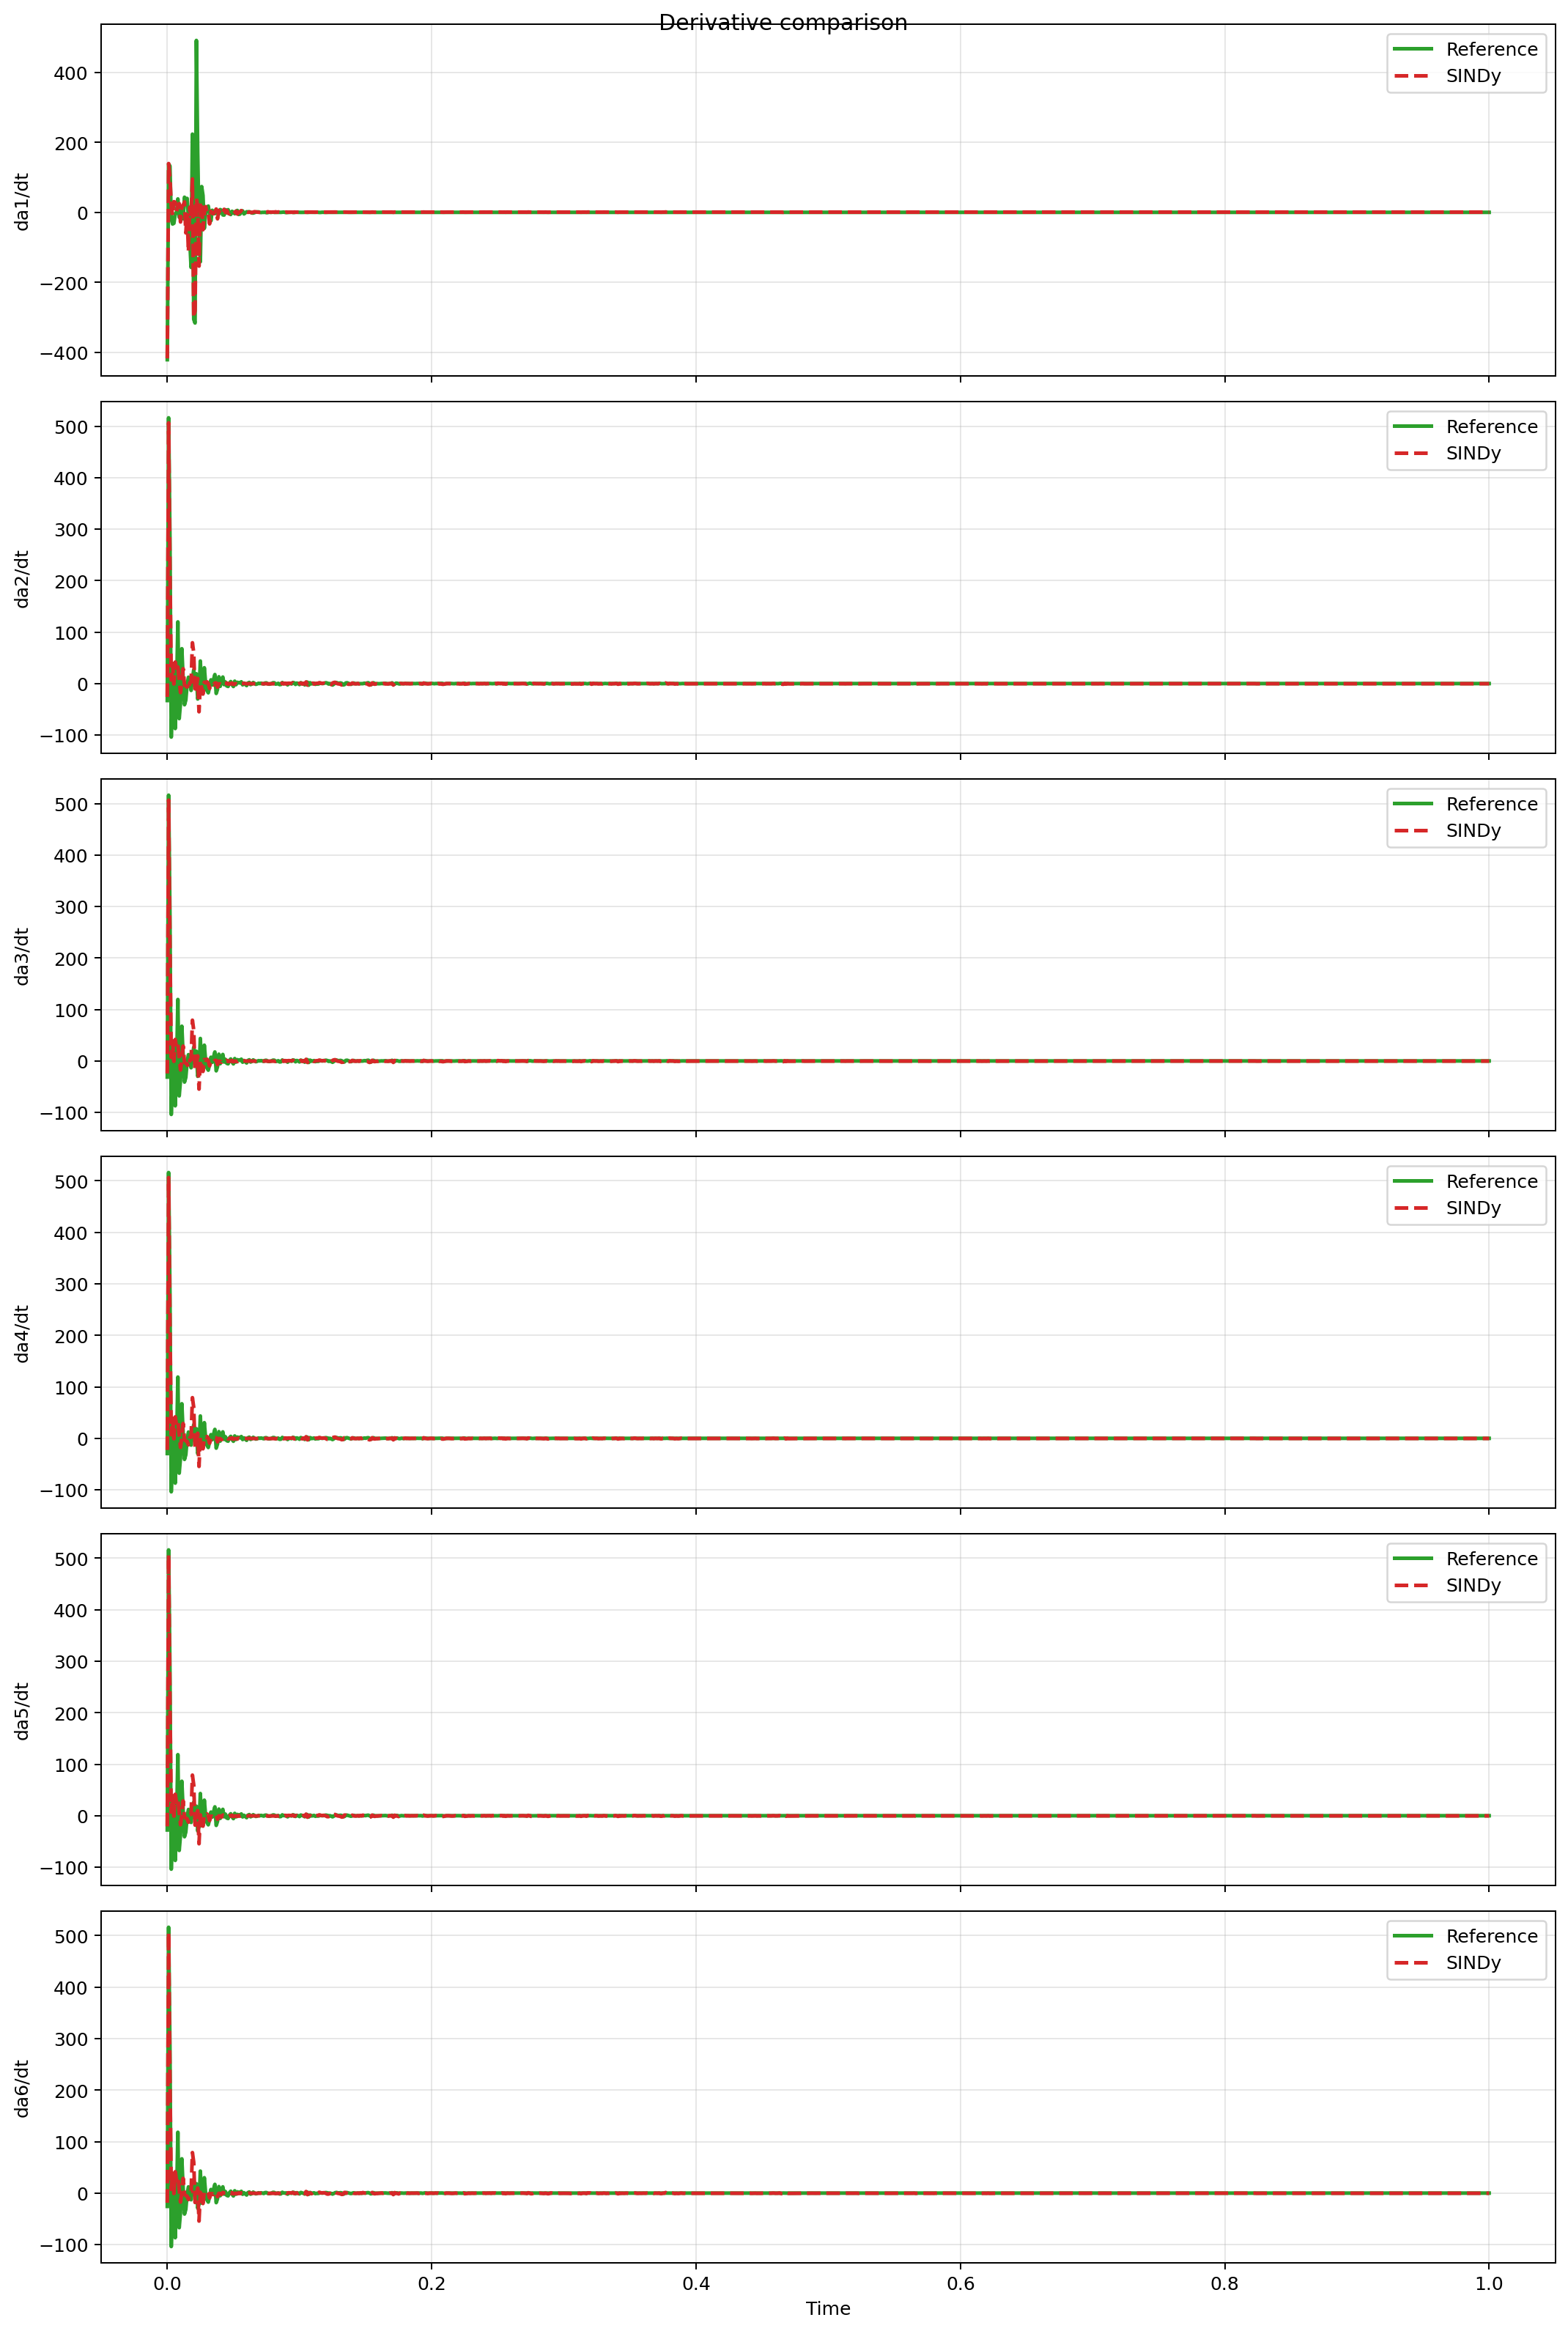
\includegraphics[width=\linewidth]{pod_sindy_deriv.png}\caption{Derivadas.}\end{subfigure}
\begin{subfigure}{0.49\textwidth}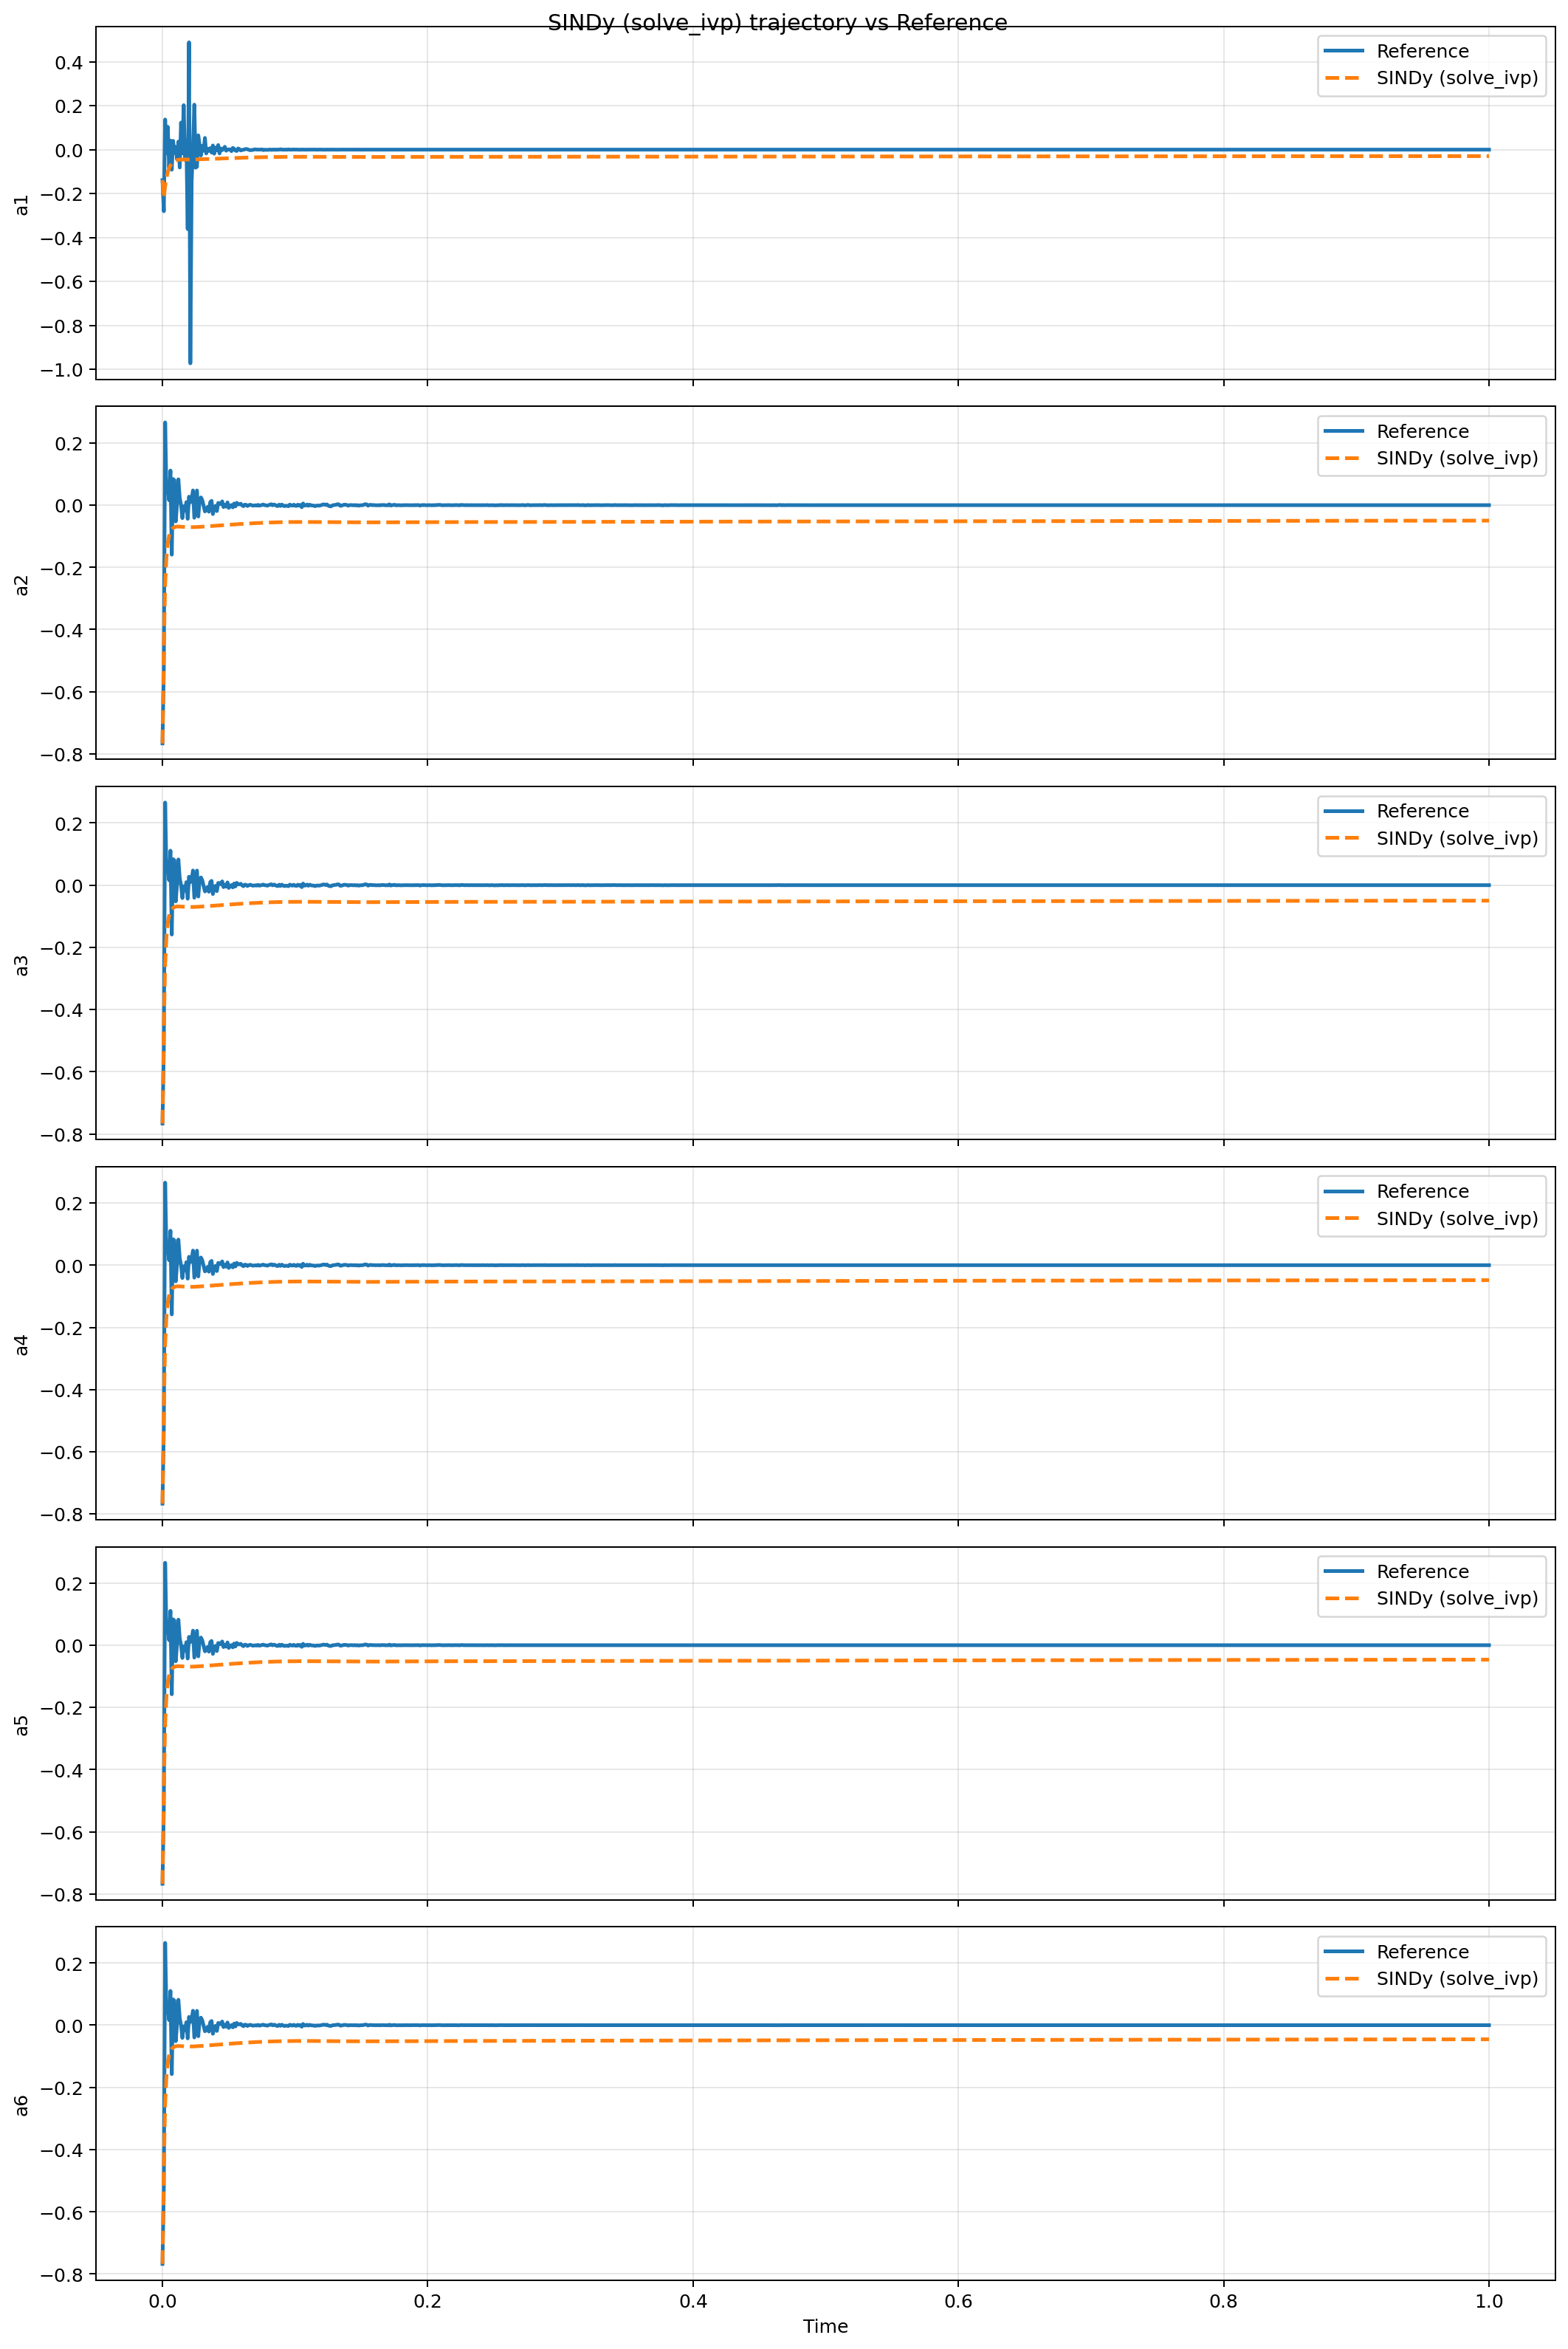
\includegraphics[width=\linewidth]{pod_sindy_traj.png}\caption{Trajetórias.}\end{subfigure}
\caption{POD--SINDy: ajuste local moderado e forte divergência na integração autônoma.}
\label{fig:podsindy}
\end{figure}

\begin{figure}[H]
\centering
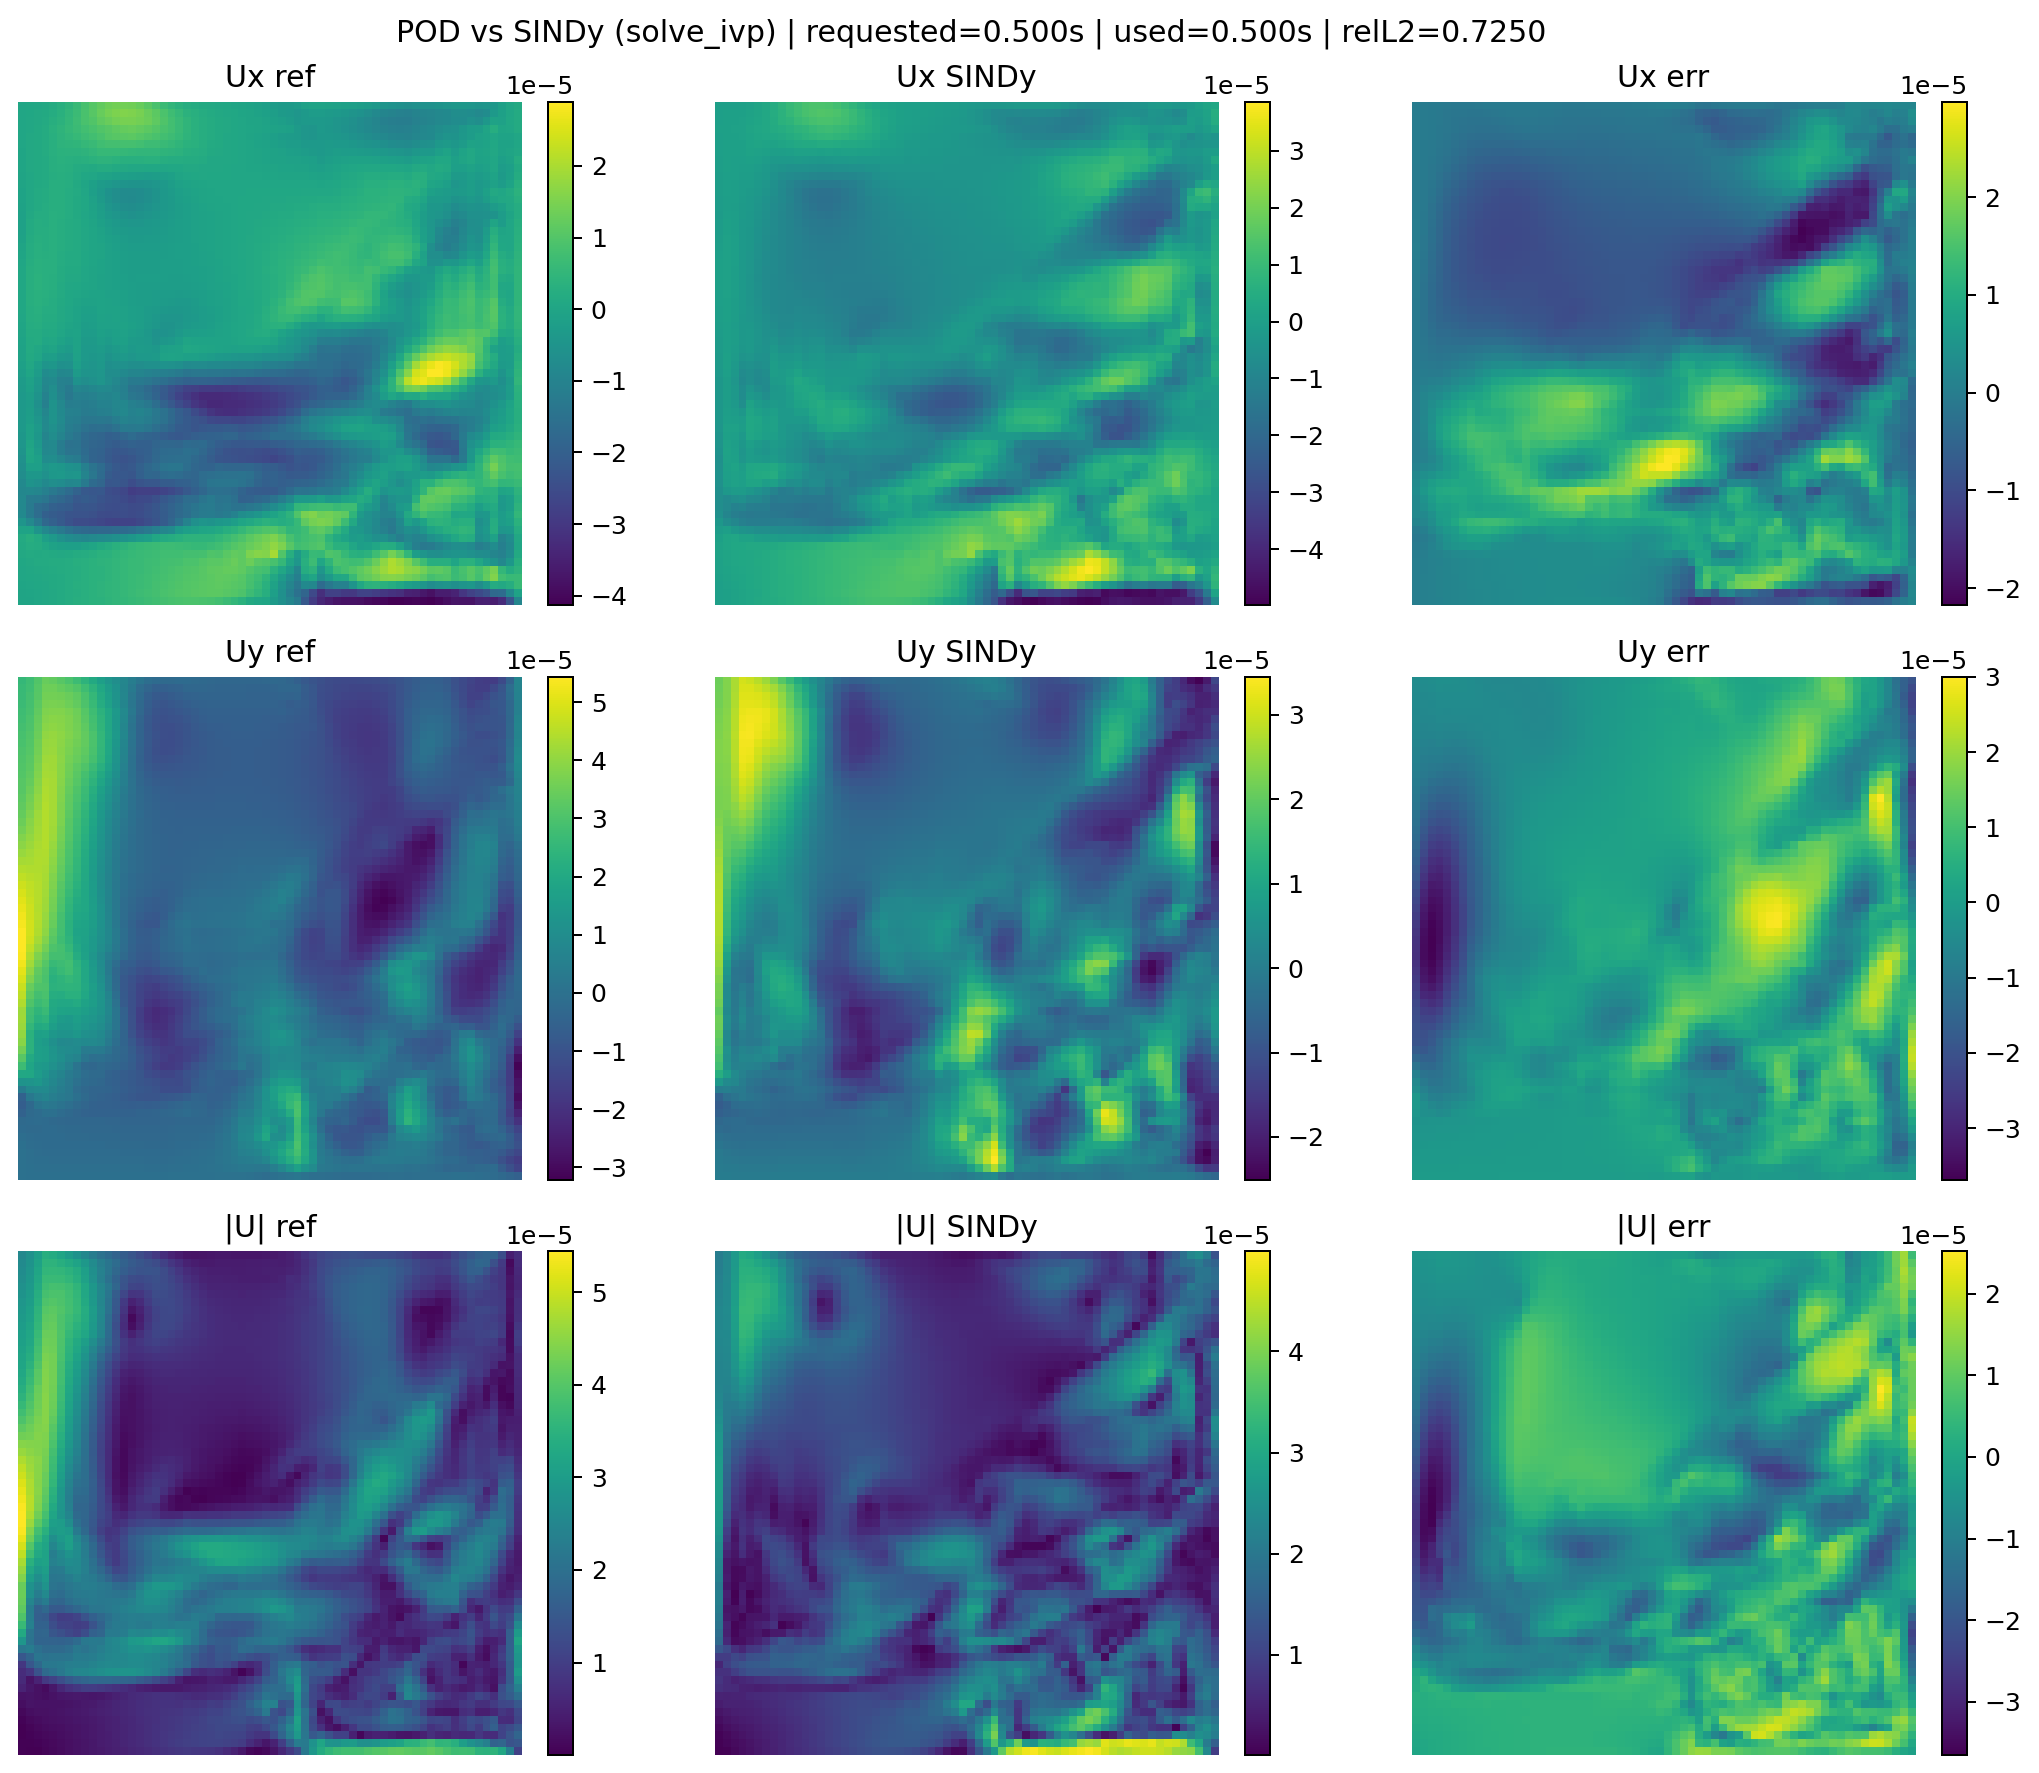
\includegraphics[width=0.9\textwidth]{pod_sindy_t05.png}
\caption{Comparação espacial POD--SINDy em $t=\SI{0.5}{s}$, conforme resultado salvo.}
\label{fig:podsindyfield}
\end{figure}

Uma busca posterior testou 84 combinações e não encontrou modelo dentro dos limites impostos. O melhor compromisso usou 16 modos (92,61\% de energia), ordem 2, seno ativo e $\alpha=0,03$: 50 termos não nulos em 2960 possíveis, erro de derivada 0,5043, erro guiado de trajetória 0,8530 e erro livre 1,6648. A alta esparsidade não se traduziu em estabilidade dinâmica.

\paragraph{Interpretação.} A POD captura estruturas lineares energéticas e o SINDy quadrático acrescenta interações não lineares entre amplitudes. Contudo, oito modos descartam 16,20\% da energia e geram erro de projeção de 40,25\%; fechamento modal, impactos e dinâmica da interface não resolvida aparecem como termos faltantes. O erro livre maior que um torna este modelo inadequado para previsão autônoma longa, embora possa ter utilidade descritiva local.

\subsection{SINDy diretamente nos latentes SAE}
O SAE--SINDy salvo foi construído sobre 101 amostras e oito latentes do SAE antigo. A biblioteca combinou polinômios de ordem 2 e seno/cosseno dos estados, totalizando 61 termos por equação. Lasso selecionou $\alpha=10^{-3}$.

\begin{table}[H]
\centering
\caption{Resultados do SAE--SINDy salvo.}
\label{tab:saesindy}
\begin{tabularx}{\textwidth}{>{\bfseries}l X}
\toprule
Item & Resultado\\
\midrule
Snapshots / $\Delta t$ & 101 / aproximadamente \SI{0.01}{s}\\
Estados & 8 latentes SAE antigos\\
Biblioteca & ordem 2 + seno/cosseno; 61 termos por equação\\
Regressão & Lasso, $\alpha=10^{-3}$\\
Coeficientes não nulos & 469 de 488 possíveis\\
Erro relativo das derivadas & 0,3661\\
Erro de trajetória reportado & 0,2314\\
Integração livre & falhou: passo requerido abaixo da precisão numérica\\
Trajetória final & \emph{fallback} de um passo guiado pela referência\\
\bottomrule
\end{tabularx}
\end{table}

\subsubsection*{Equações descobertas: SAE--SINDy}
As variáveis $z_1,\ldots,z_8$ são as coordenadas do SAE antigo. O sistema inclui constantes, termos lineares, quadráticos e funções trigonométricas. A listagem integral deixa visível a baixa esparsidade: quase toda a biblioteca foi mantida.
\lstinputlisting[style=sindyeq,caption={Sistema completo identificado diretamente nos latentes SAE.},label={lst:eqsaesindy}]{equacoes_sae_sindy.txt}

\begin{figure}[H]
\centering
\begin{subfigure}{0.49\textwidth}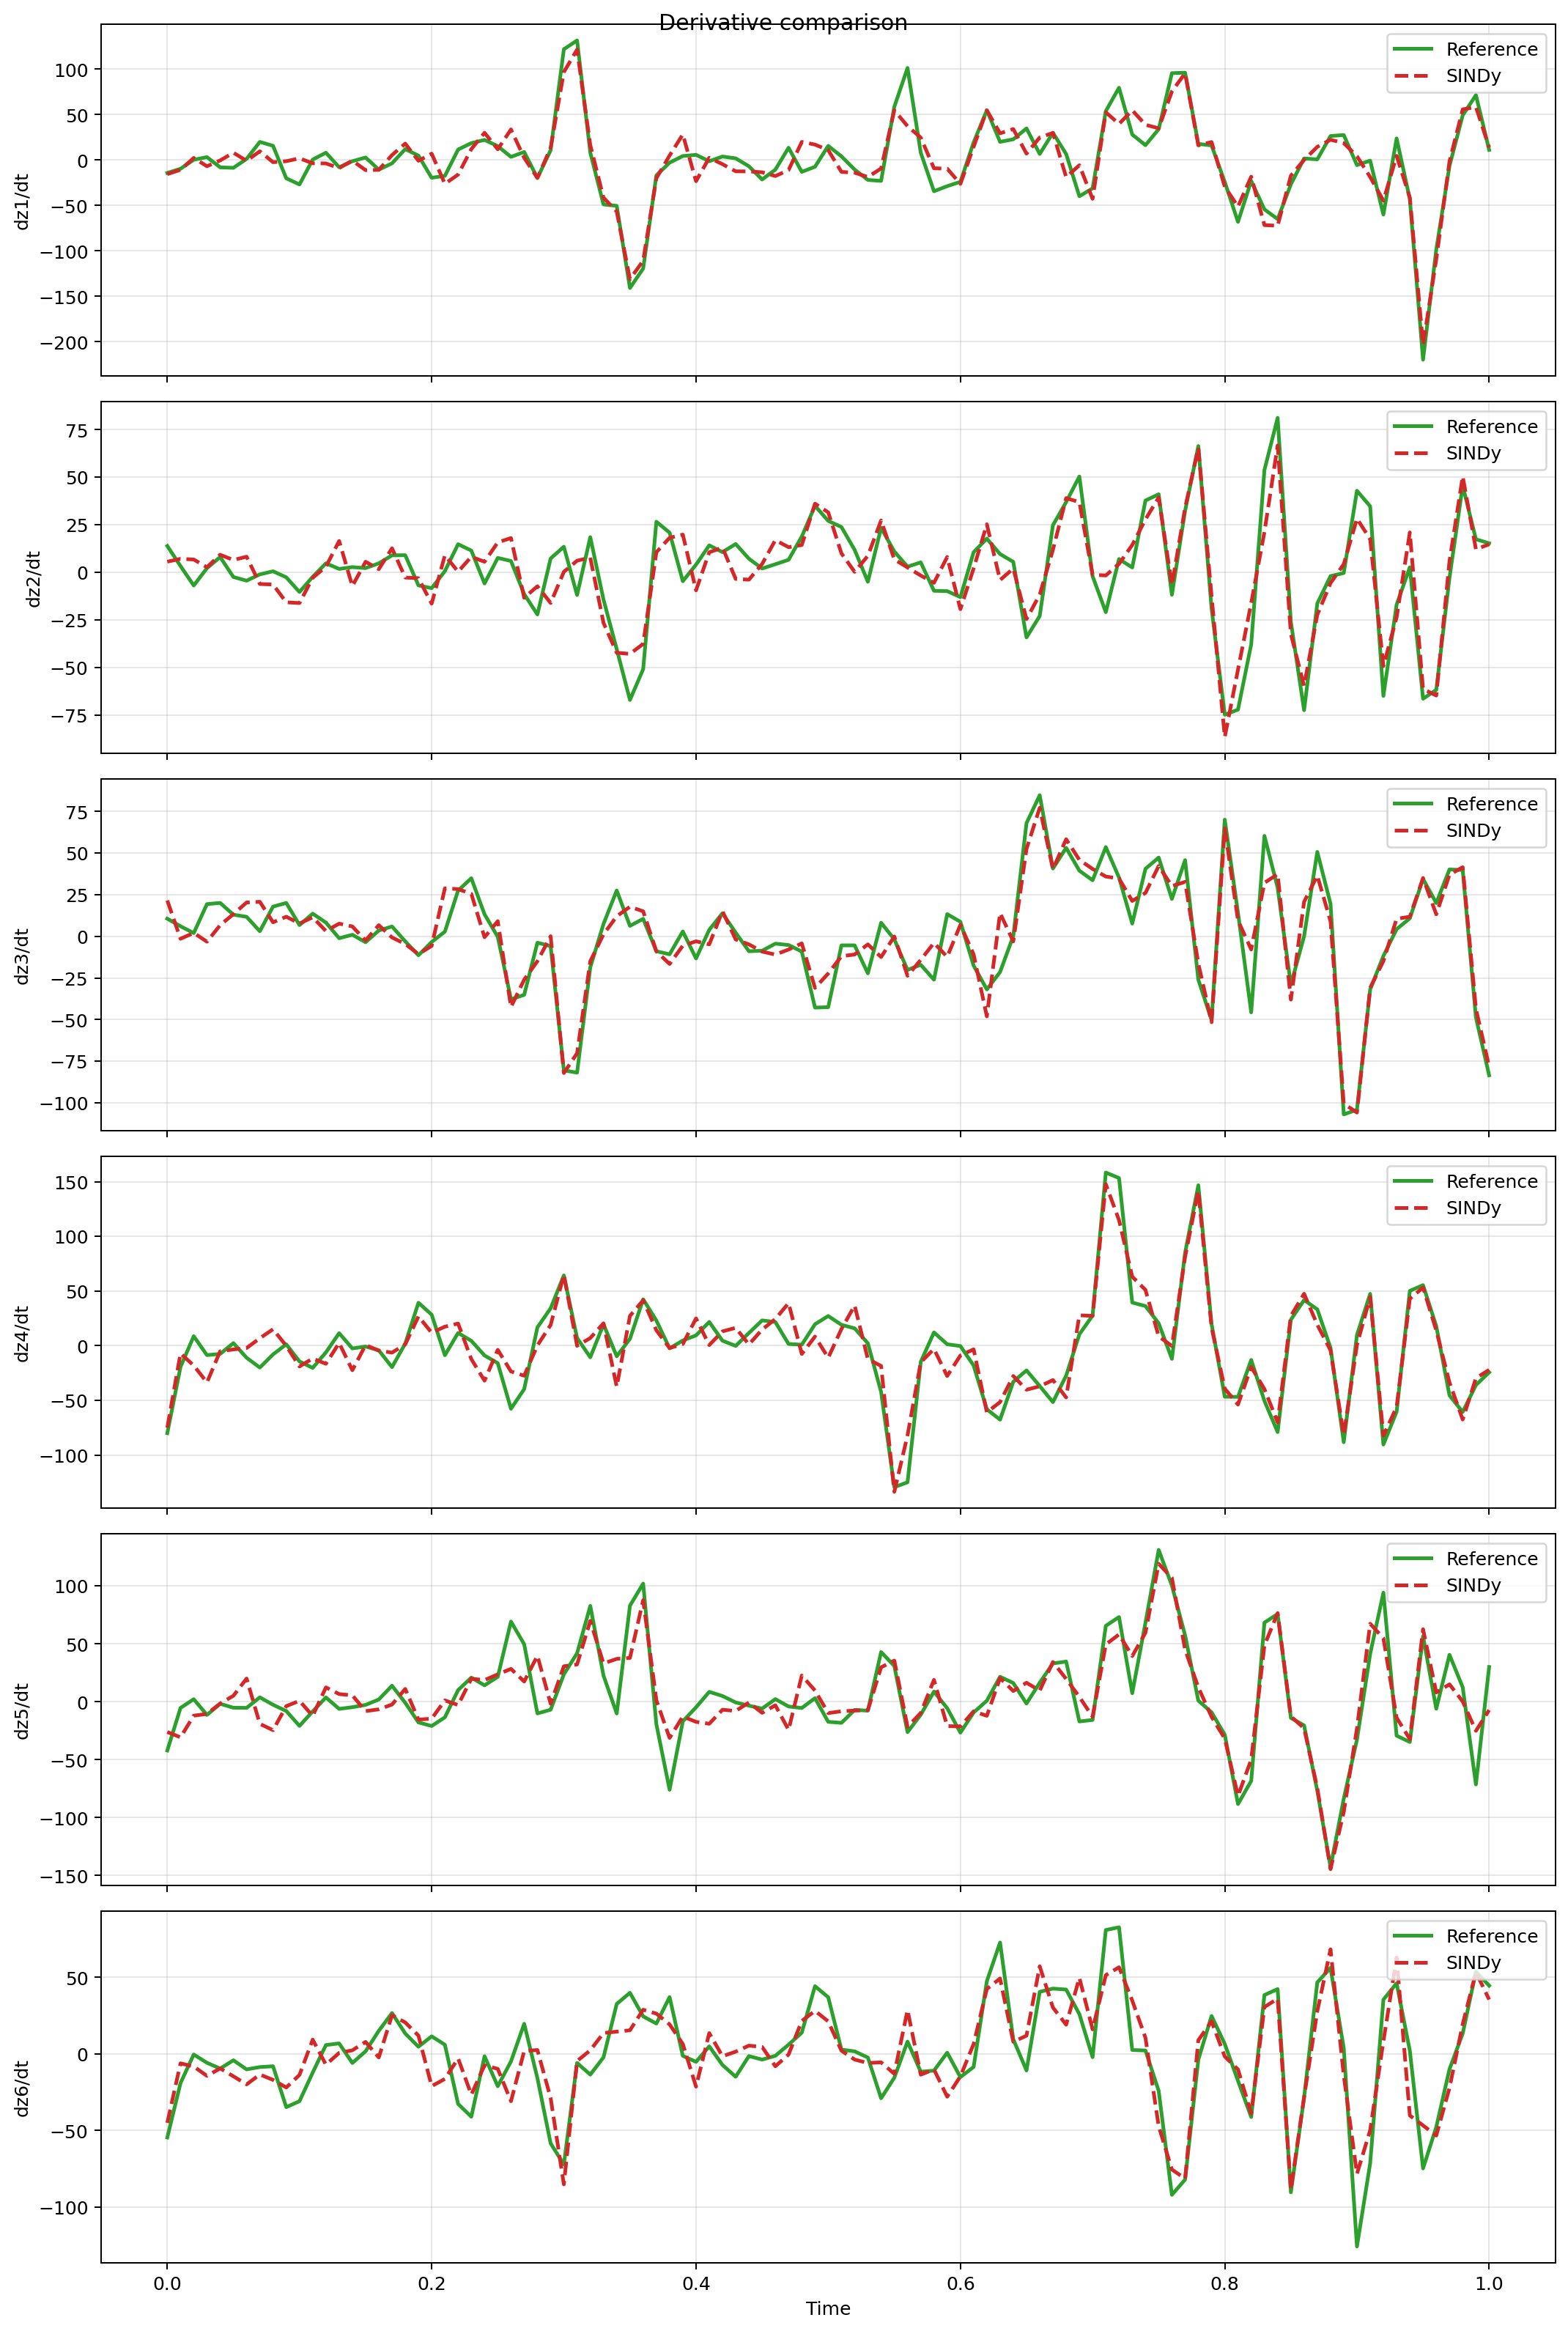
\includegraphics[width=\linewidth]{sae_sindy_deriv.png}\caption{Derivadas latentes.}\end{subfigure}
\begin{subfigure}{0.49\textwidth}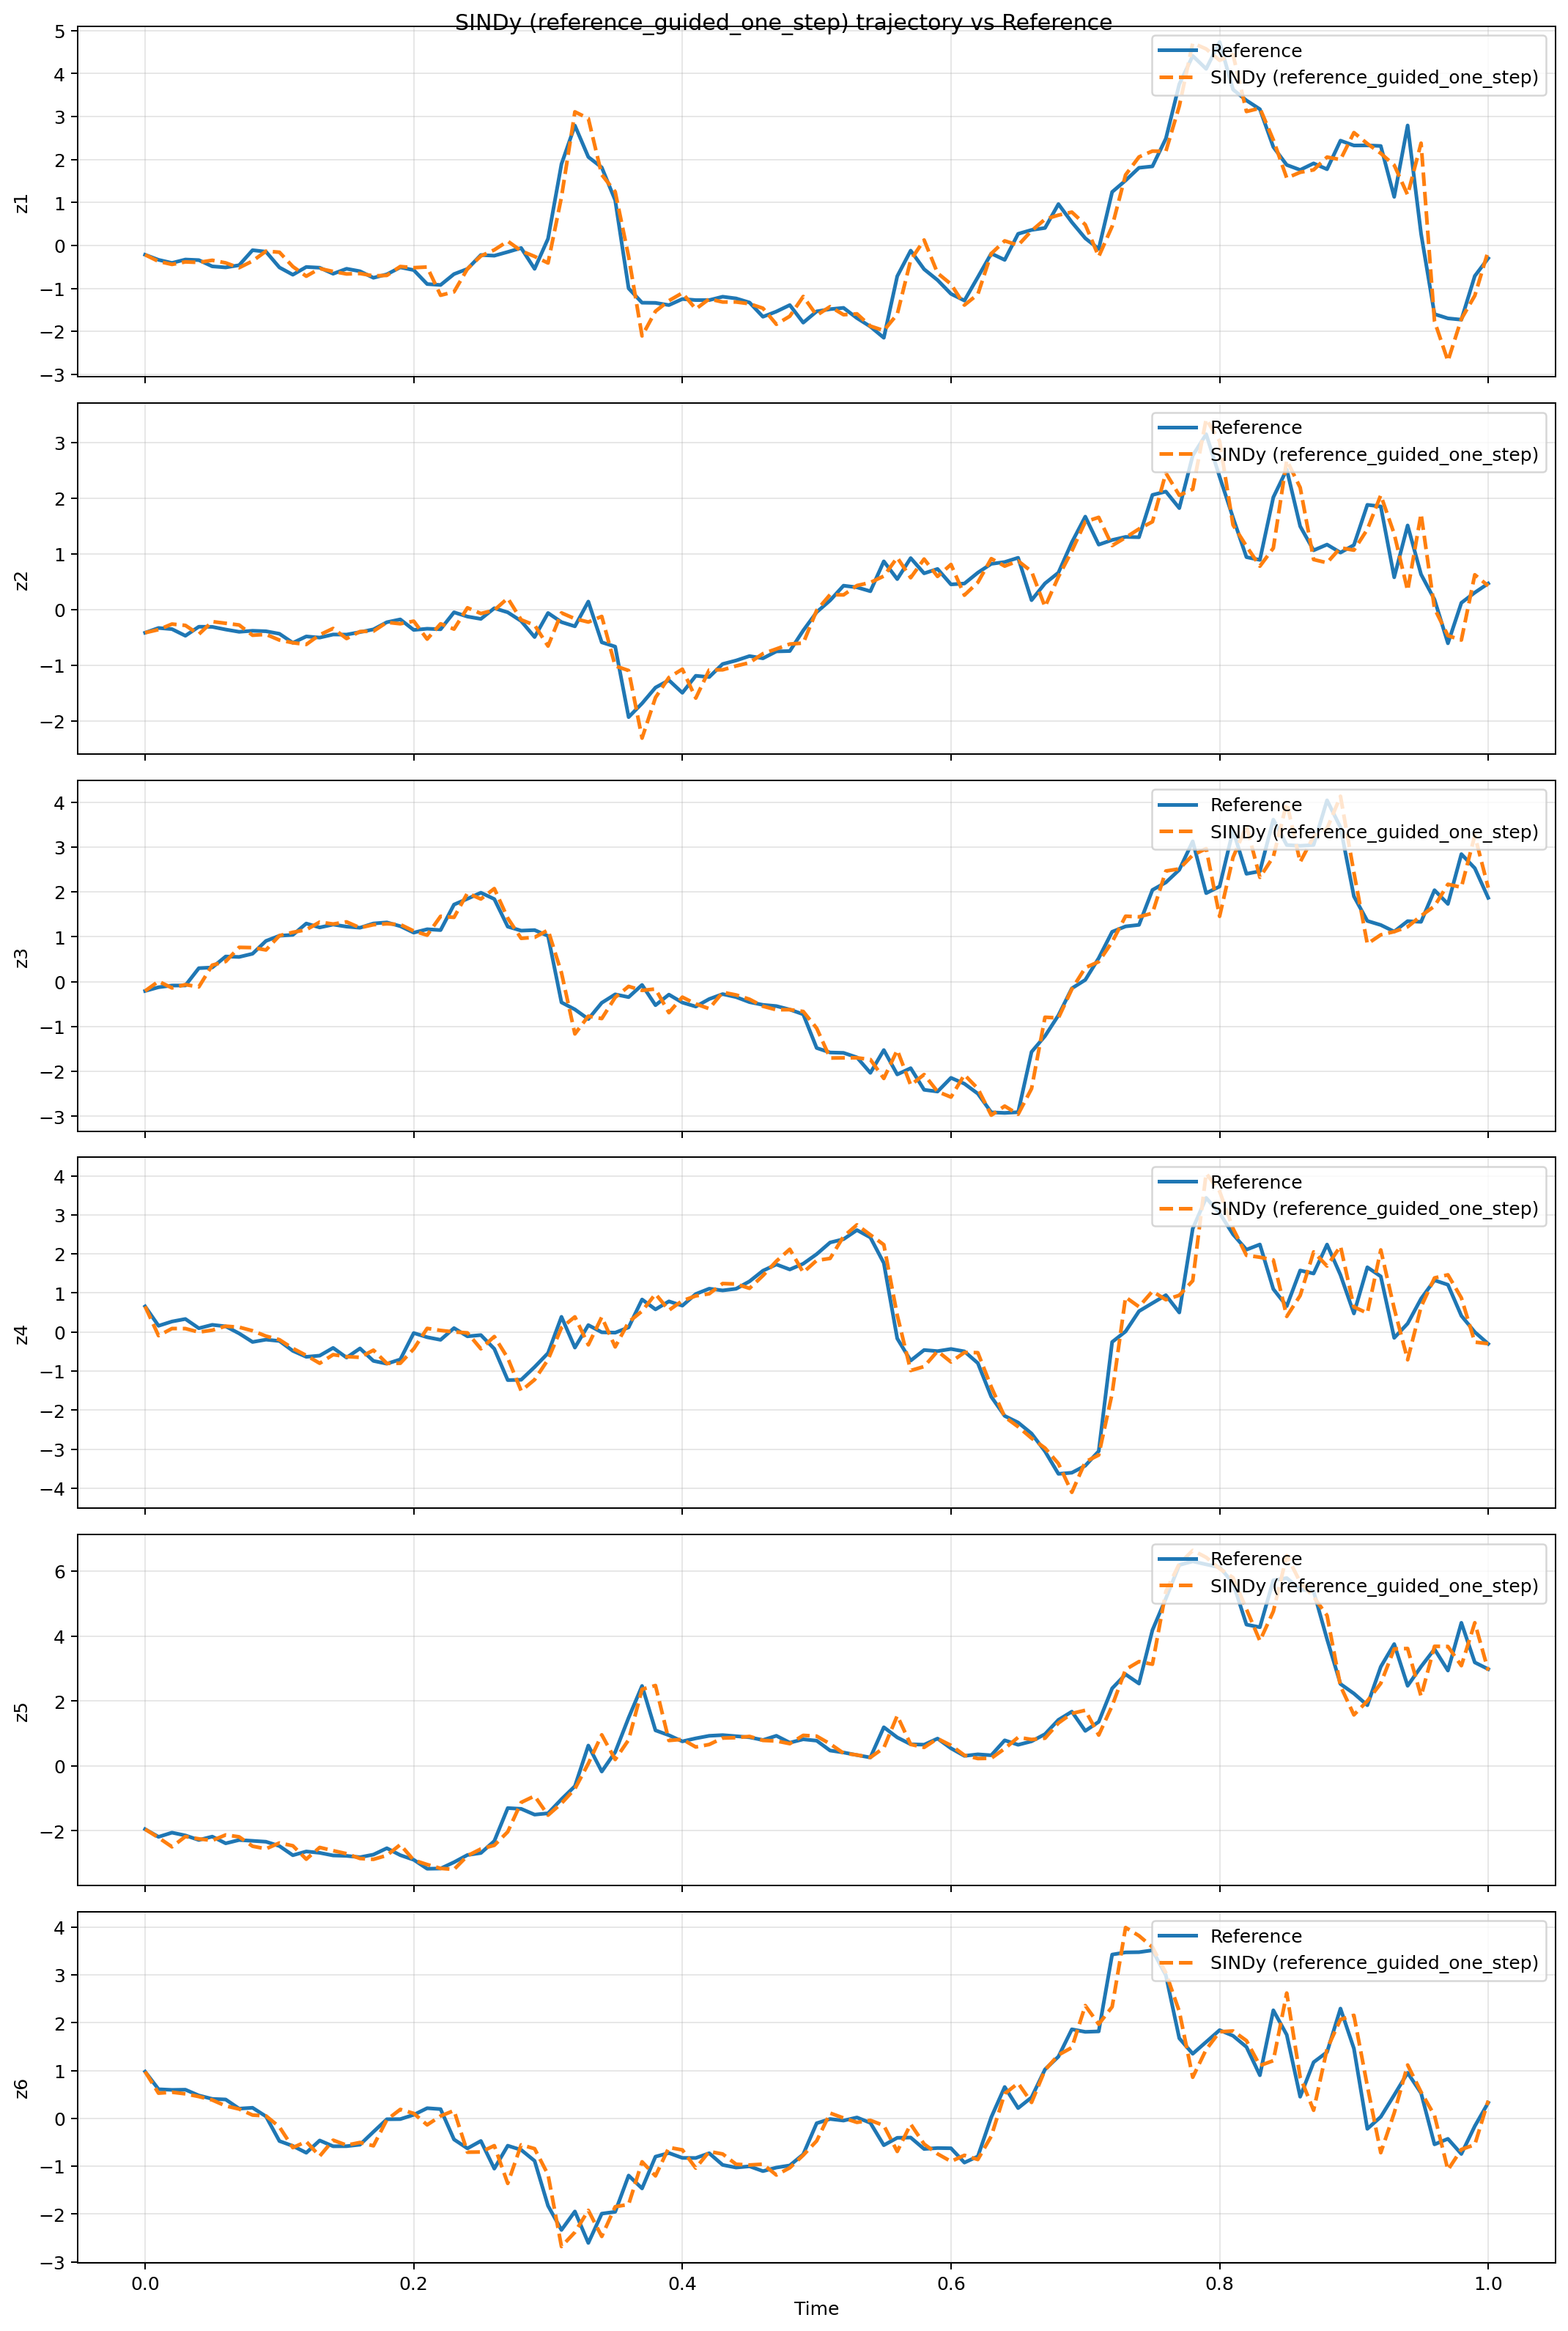
\includegraphics[width=\linewidth]{sae_sindy_traj.png}\caption{Trajetória guiada.}\end{subfigure}
\caption{SAE--SINDy antigo. O erro de trajetória não corresponde a uma integração autônoma bem-sucedida.}
\label{fig:saesindy}
\end{figure}

\paragraph{Interpretação.} O erro de derivada é menor que no POD--SINDy principal, sinal de que o espaço não linear pode alinhar melhor alguns movimentos. Porém, 469 de 488 coeficientes são não nulos: o modelo praticamente não é esparso, perde interpretabilidade e apresenta rigidez/instabilidade suficiente para interromper a integração. A curva guiada usa o estado verdadeiro no início de cada passo e, portanto, não deve ser apresentada como previsão livre.

\subsection{SAE--POD--SINDy: POD como estabilizador}
Nesta arquitetura, os latentes SAE antigos são padronizados e submetidos a uma segunda SVD. Quatro coordenadas POD latentes $r_i$ preservam 88,45\% da energia. A ideia é remover direções latentes ruidosas/correlacionadas antes da diferenciação e obter um sistema de menor dimensão.

O melhor resultado salvo usa biblioteca de ordem 1, Lasso adaptativo, $\alpha=10^{-3}$, Savitzky--Golay com janela 51, termos polinomiais e harmônicos explícitos no tempo, frequência $0,9901$, sem senos dos estados e integrador RK45. A dependência explícita de $t$ torna o modelo não autônomo: ele pode ajustar fases/transientes, mas reduz a universalidade das equações.

\begin{table}[H]
\centering
\caption{Métricas do SAE--POD--SINDy selecionado.}
\label{tab:hybrid}
\begin{tabular}{lr}
\toprule
Métrica & Valor\\
\midrule
Energia POD nos latentes (4 modos) & 0,8845\\
Biblioteca / coeficientes não nulos & 10 / 33 de 40\\
Erro $L_2$ das derivadas & 0,1871\\
$R^2$ das derivadas & 0,9650\\
Erro $L_2$ de um passo & 0,3593\\
$R^2$ de um passo & 0,8709\\
Erro $L_2$ da integração livre & 0,8578\\
$R^2$ da integração livre & 0,2641\\
$R^2$ um passo: treino / validação & 0,9144 / 0,5933\\
\bottomrule
\end{tabular}
\end{table}

\subsubsection*{Equações descobertas: SAE--POD--SINDy}
Neste sistema, $r_1,\ldots,r_4$ são as quatro coordenadas POD obtidas dos latentes SAE padronizados. Além dos acoplamentos lineares, aparecem $t$, $t^3$ e termos harmônicos com frequência identificada $0,9901$. Assim, estas equações são não autônomas e incorporam explicitamente a fase temporal do experimento.
\lstinputlisting[style=sindyeq,caption={Sistema identificado após estabilização dos latentes SAE por POD.},label={lst:eqhibrido}]{equacoes_sae_pod_sindy.txt}

Nenhuma das 48 configurações testadas satisfez os critérios de aceitação; o resultado foi escolhido por possuir o menor erro livre disponível. Portanto, ``melhor'' significa melhor dentro da busca, não modelo validado.

\begin{figure}[H]
\centering
\begin{subfigure}{0.49\textwidth}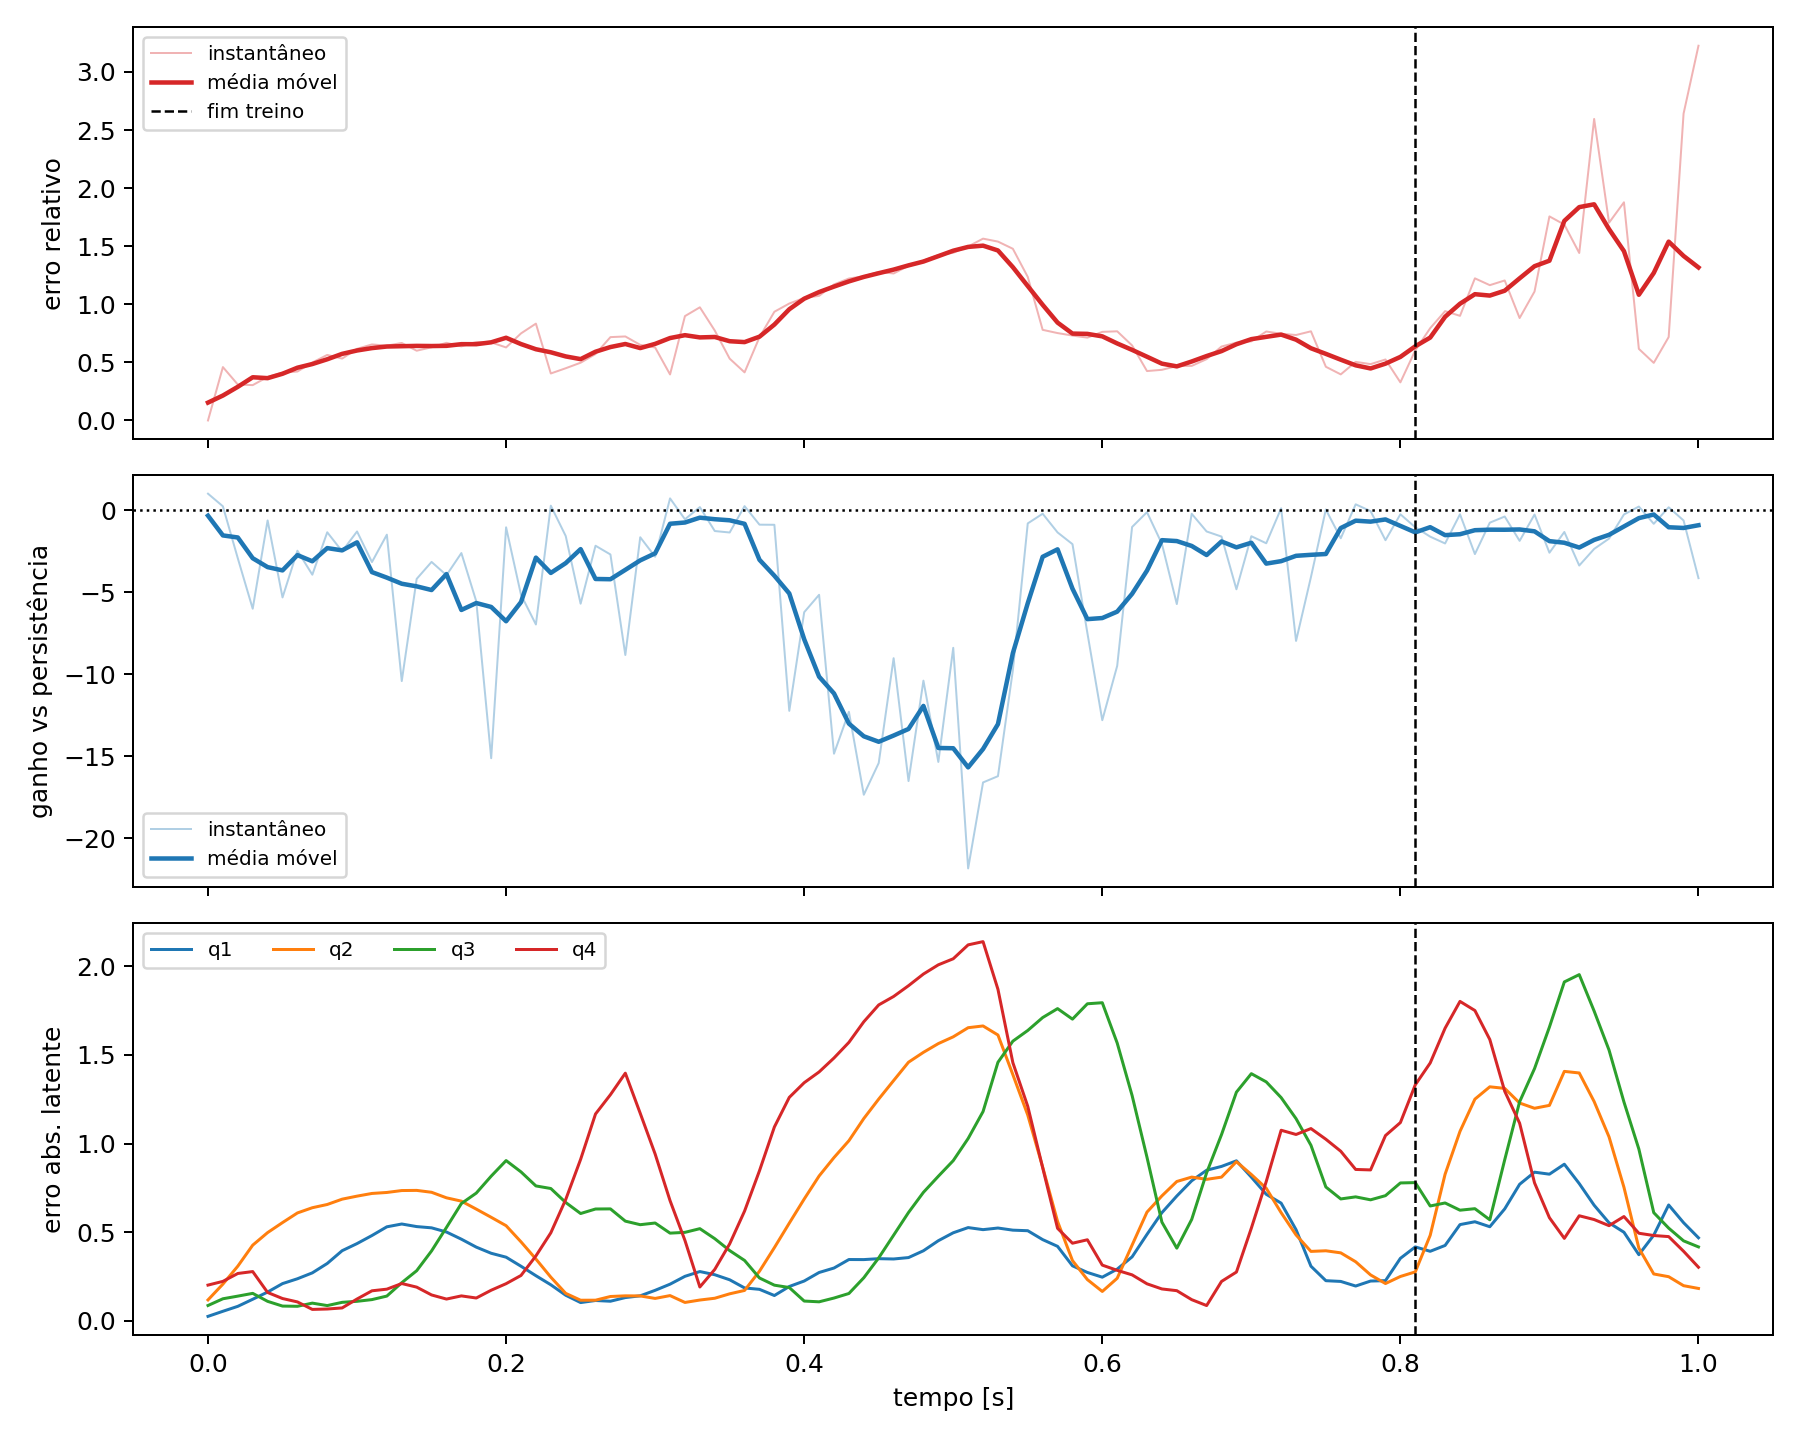
\includegraphics[width=\linewidth]{hibrido_erro_temporal.png}\caption{Erro e ganho temporal.}\end{subfigure}
\begin{subfigure}{0.49\textwidth}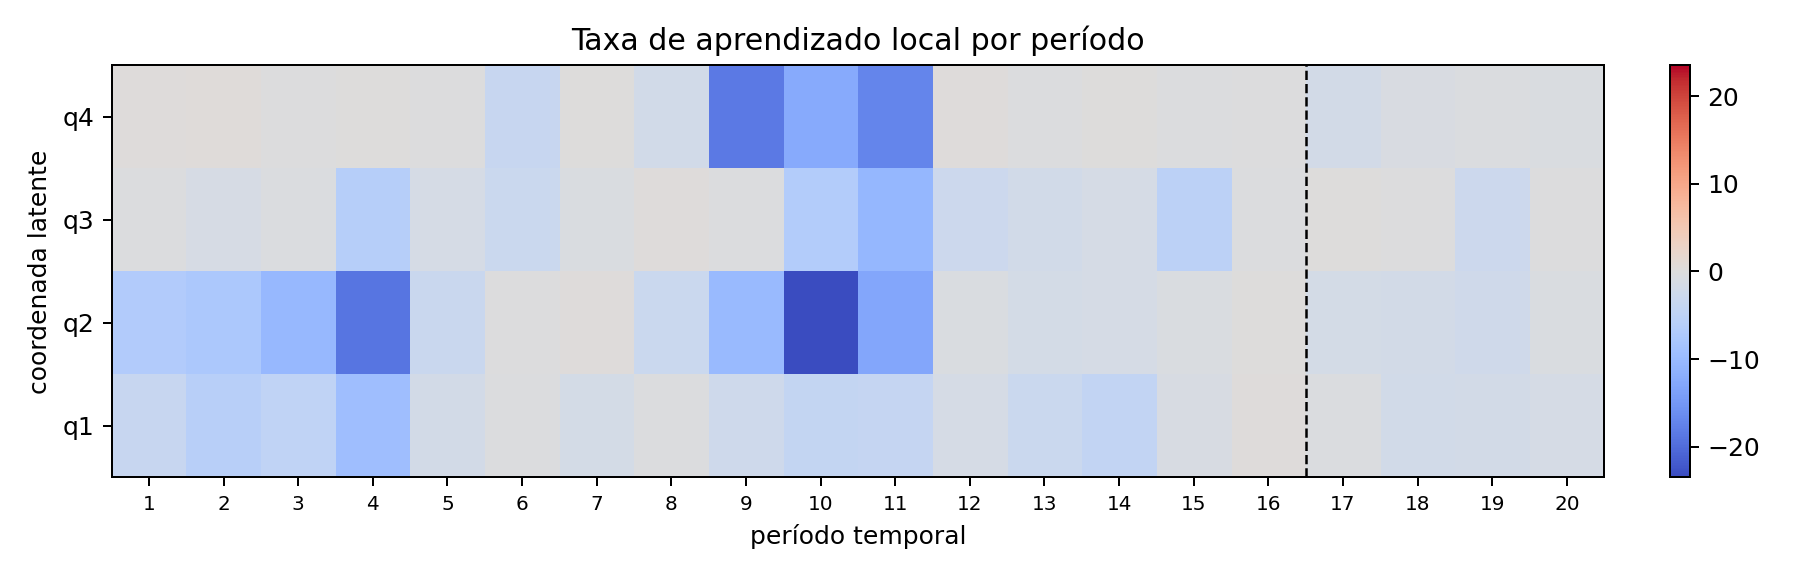
\includegraphics[width=\linewidth]{hibrido_mapa_aprendizado.png}\caption{Mapa temporal das coordenadas.}\end{subfigure}
\caption{Diagnóstico temporal do SAE--POD--SINDy.}
\label{fig:hybdiag}
\end{figure}

\begin{figure}[H]
\centering
\begin{subfigure}{0.49\textwidth}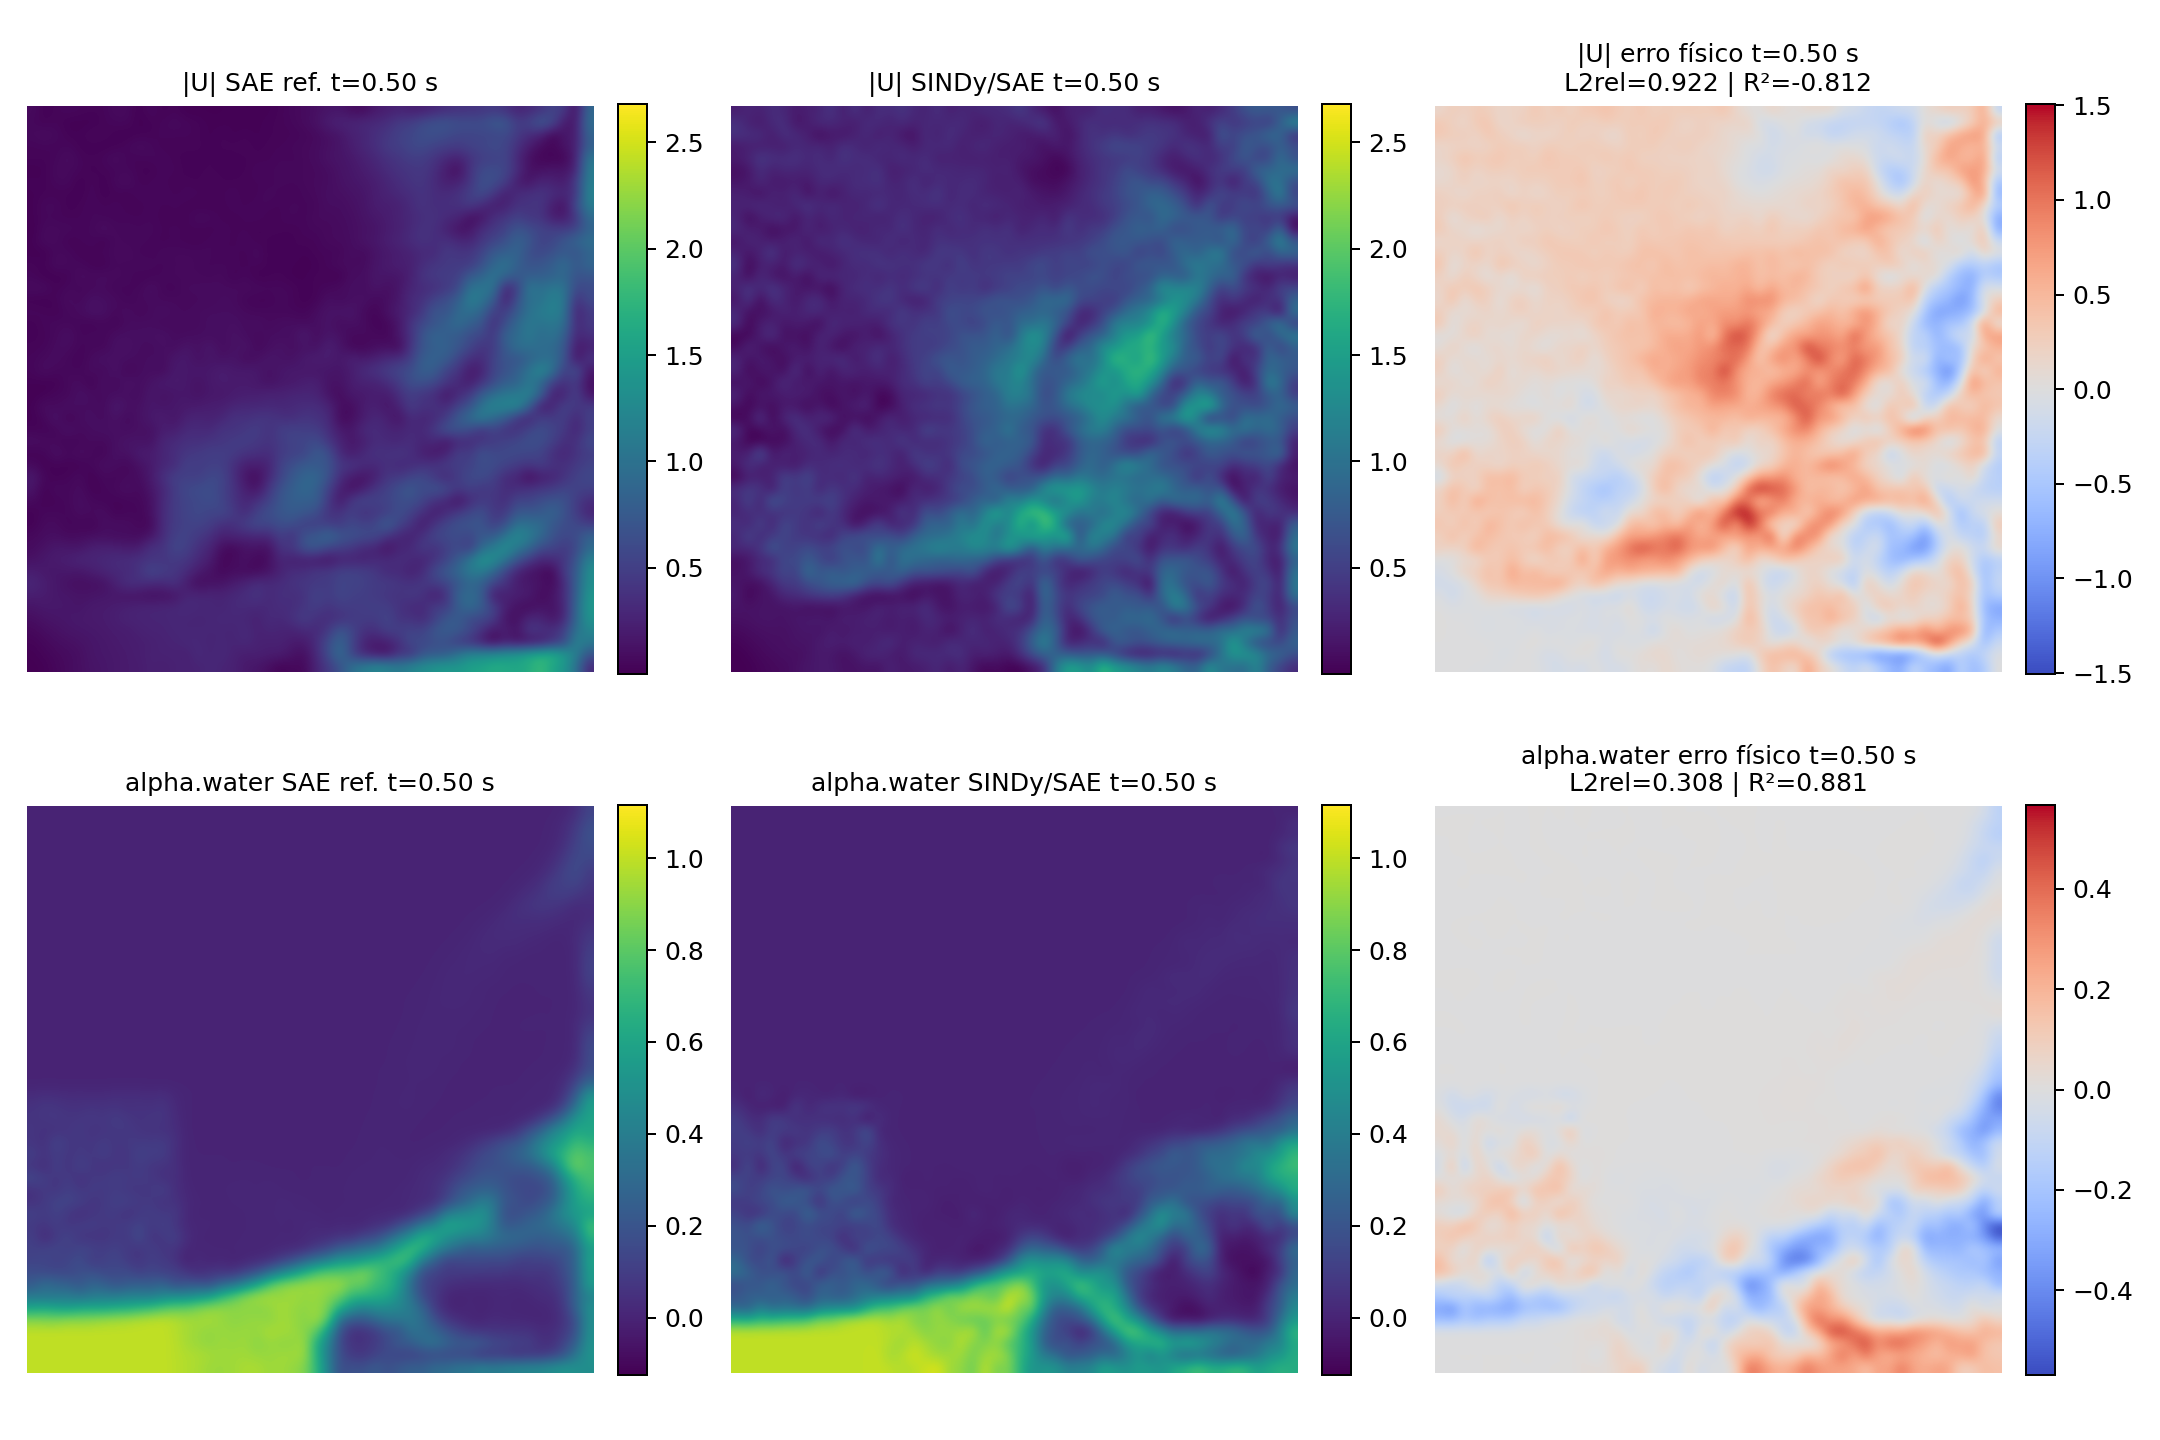
\includegraphics[width=\linewidth]{hibrido_t05.png}\caption{$t=\SI{0.5}{s}$.}\end{subfigure}
\begin{subfigure}{0.49\textwidth}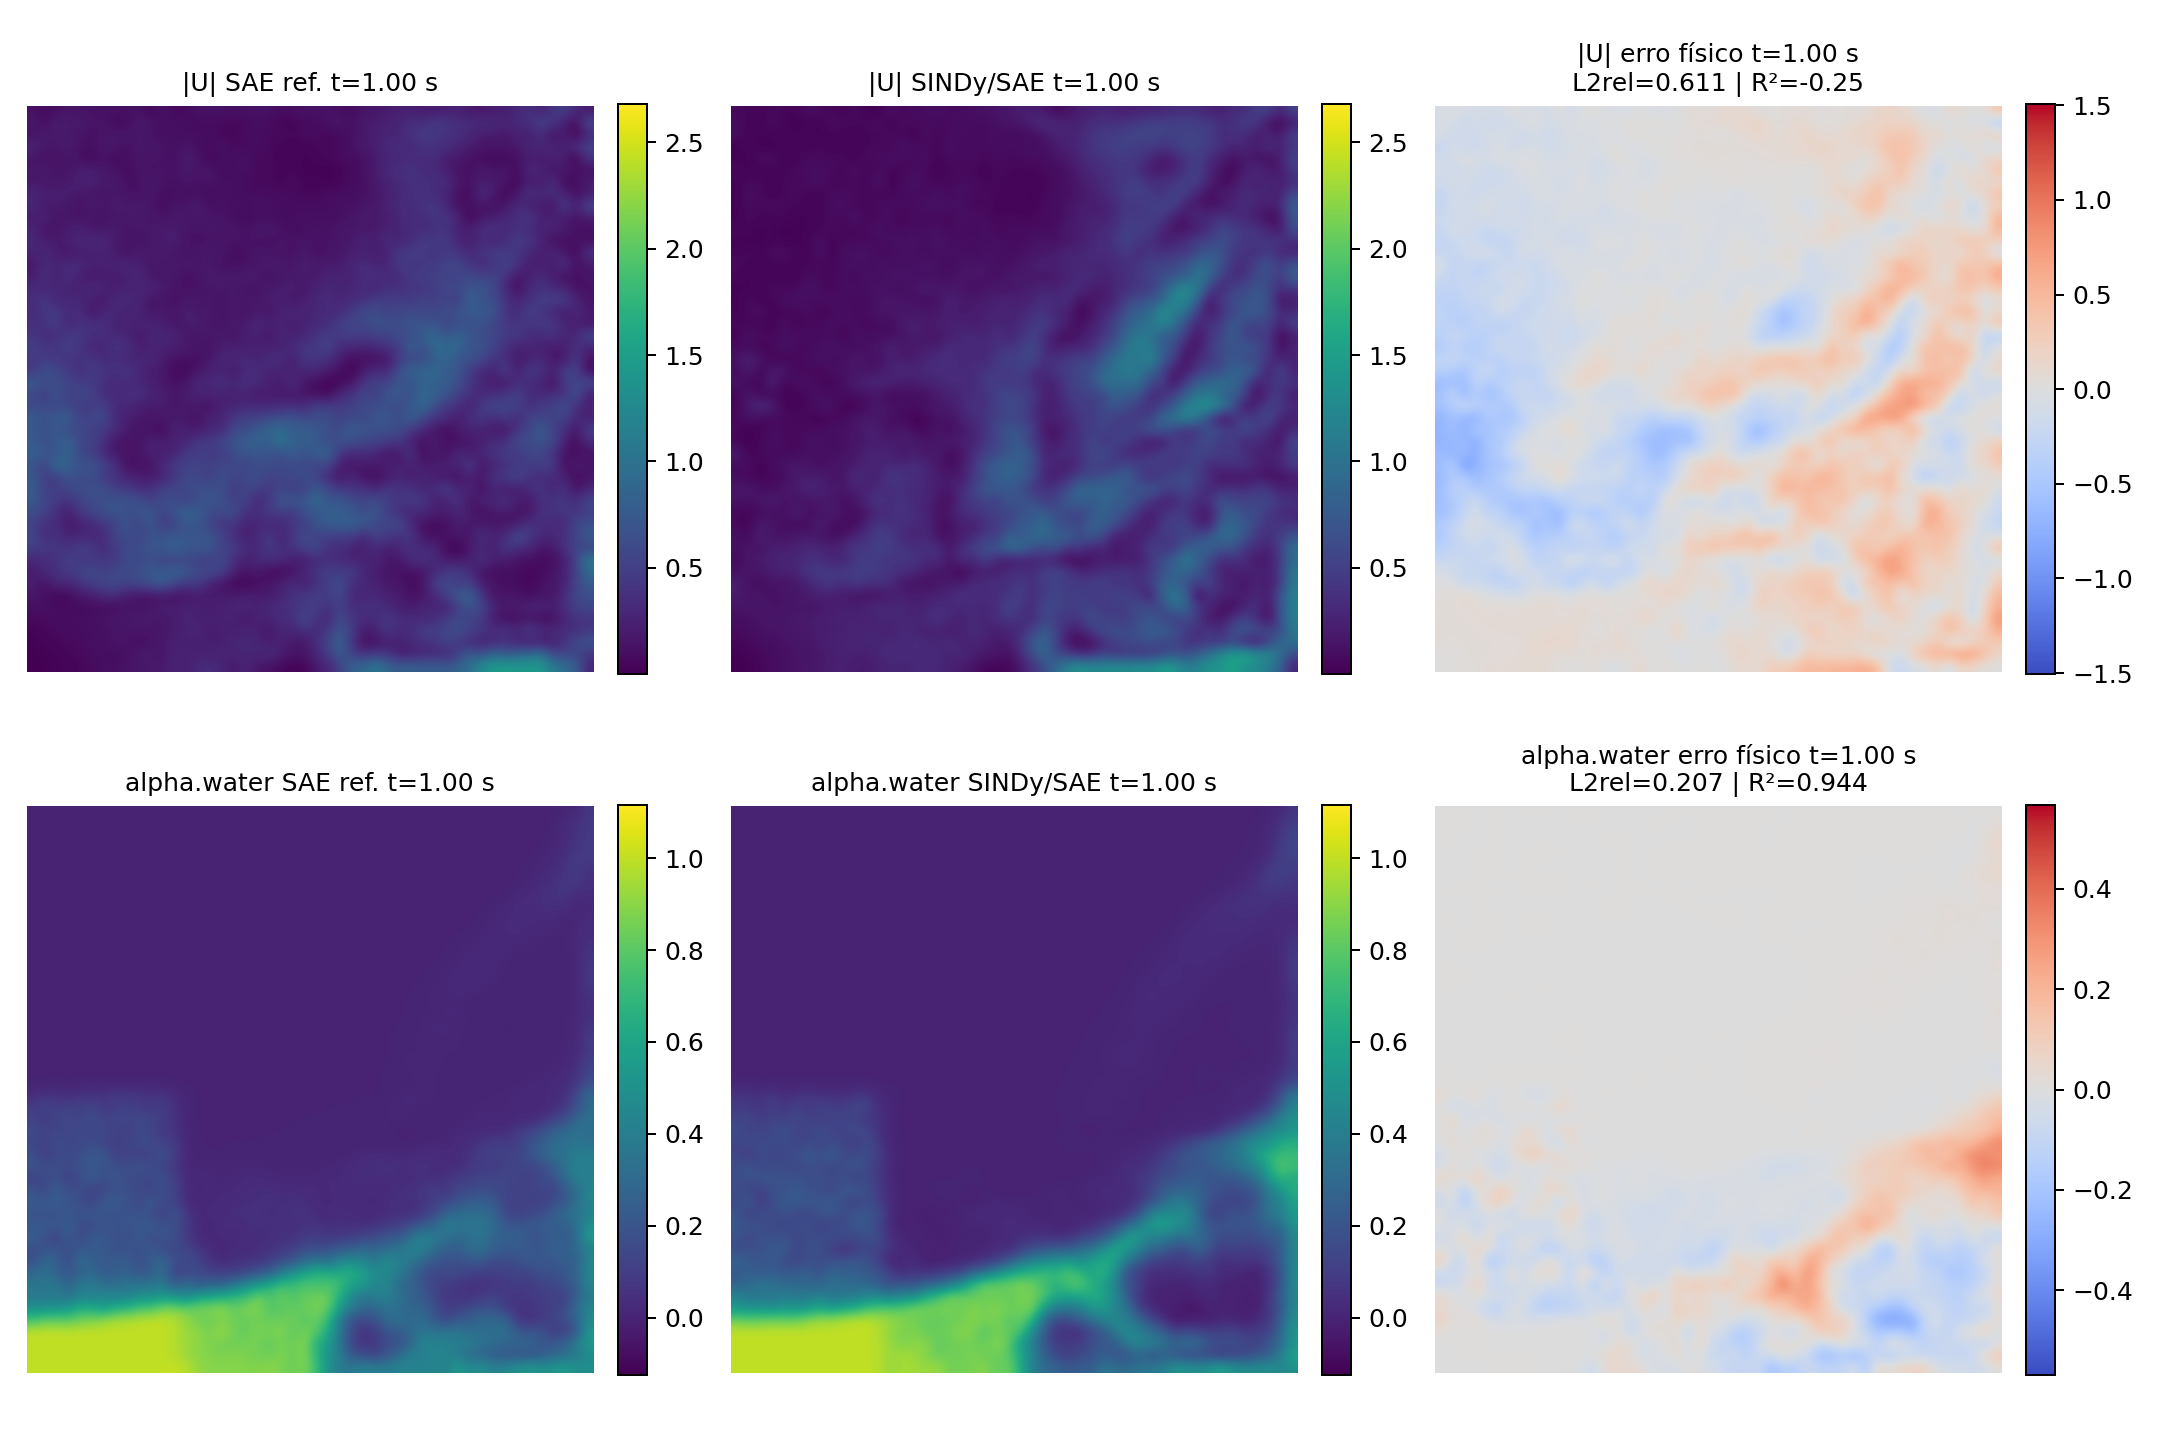
\includegraphics[width=\linewidth]{hibrido_t10.png}\caption{$t=\SI{1.0}{s}$.}\end{subfigure}
\caption{Campos decodificados pela integração livre do SAE--POD--SINDy. A interface é melhor preservada que a velocidade em alguns instantes.}
\label{fig:hybfields}
\end{figure}

Nos cinco tempos examinados, o erro de $\alpha_{water}$ variou de 0,096 a 0,308, com $R^2$ de 0,881 a 0,989. Para $|U|$, o erro variou de 0,156 a 0,922; em $t=0,5$ e $1,0\,\si{s}$, $R^2$ foi negativo. Isso mostra que a posição/forma global da fase é reconstruída com mais robustez que os detalhes da velocidade.

Um segundo relatório denominado \code{openfoam\_raw\_vs\_sindy} contém erros gigantes, da ordem de $10^4$ a $10^{13}$. Esses números são incompatíveis com as comparações decodificadas e indicam problema de escala/proveniência no caminho de comparação direta com o cache OpenFOAM; eles não foram usados como medida física válida neste relatório.

\paragraph{Efeito estabilizador da POD.} A POD latente reduz 8 coordenadas para 4, melhora o condicionamento, permite integração RK45 até o fim e reduz o erro de derivada de 0,366 para 0,187 em relação ao SAE--SINDy salvo. Isso é um ganho real no ajuste local. Entretanto, o erro livre 0,858 e o $R^2$ livre 0,264 mostram que a estabilização é parcial: ruído e redundância foram reduzidos, mas fechamento, generalização e acúmulo de erro continuam problemáticos.

\section{Comparação integrada: linearidade, não linearidade e previsão}

\begin{table}[H]
\centering
\caption{Síntese qualitativa dos métodos.}
\label{tab:sintese}
\begin{tabularx}{\textwidth}{>{\bfseries}l X X X}
\toprule
Método & O que captura bem & Limitação principal & Dinâmica\\
\midrule
POD & estruturas globais energéticas; erro controlável pelo número de modos & subespaço linear; frentes móveis exigem muitos modos & redução linear, sem lei temporal própria\\
SAE & variedade espacial não linear; excelente reconstrução do treino após correção & forte \emph{gap} temporal e latente não condicionado para dinâmica & redução não linear, mas não garante evolução simples\\
POD--SINDy & interações polinomiais entre amplitudes POD; interpretabilidade moderada & truncamento e fechamento modal; erro livre 1,65 & não linear quadrática sobre coordenadas lineares\\
SAE--SINDy & menor erro local de derivada que POD--SINDy principal & quase não esparso; integração livre falha & não linear em espaço não linear, porém rígida/instável\\
SAE--POD--SINDy & melhor ajuste de derivadas; integração completa; menor dimensão & erro livre 0,858; nenhum candidato aceito; dependência explícita do tempo & linearização/filtragem local dos latentes + dinâmica não autônoma\\
\bottomrule
\end{tabularx}
\end{table}

\paragraph{Dinâmicas lineares.} A POD é especialmente eficiente quando a evolução permanece próxima a um subespaço linear e poucos modos dominam a energia. Neste caso, os primeiros oito modos ainda deixam erro de 40,25\%, indicando que o transiente de dam-break não é bem descrito por uma base linear muito curta. Termos lineares no SINDy representam crescimento, decaimento e acoplamento modal local, mas não bastam para impacto e transporte de interface.

\paragraph{Dinâmicas não lineares.} Bibliotecas quadráticas representam interações de pares de modos; senos/cossenos podem representar oscilações, mas aumentam colinearidade e densidade. O SAE tem maior liberdade geométrica, mas o SINDy sobre seus latentes ficou denso e instável. Isso demonstra que ``redução não linear'' não implica automaticamente ``dinâmica reduzida simples''. A POD estabilizadora remove direções de baixa energia e melhora derivadas, mas o uso de termos explícitos em tempo sugere que o sistema reduzido autônomo ainda não foi fechado.

\section{Os casos isolados representam dados ou dinâmica?}
A resposta depende da etapa considerada. A POD isolada e o SAE isolado são, nos códigos analisados, modelos de \textbf{representação}: eles recebem snapshots e minimizam erro de projeção/reconstrução. Não existe nessas duas etapas uma equação de evolução que permita obter o estado futuro somente a partir de uma condição inicial. Assim, energia POD, perda Huber, MSE e $R^2$ de reconstrução comprovam capacidade de representar os dados, mas não comprovam captura da dinâmica.

Os casos POD--SINDy e SAE--SINDy não são apenas reconstruções: ambos tentam identificar uma lei dinâmica. Entretanto, usando a distinção representação--descoberta dinâmica de Lin, Xiao e Fang~\cite{lin2024}, os resultados mostram que a dinâmica não foi capturada de maneira estável:
\begin{itemize}
  \item no POD--SINDy, o erro das derivadas é 0,494, mas o erro da trajetória livre chega a 1,652. O modelo representa parcialmente tendências locais dos coeficientes, porém não sustenta a evolução acumulada;
  \item no SAE--SINDy, o erro de derivada é 0,366 e o erro guiado é 0,231, mas a integração livre falha. Como o \emph{fallback} reinicializa cada passo com a referência, essa métrica demonstra ajuste local aos dados e não previsão dinâmica autônoma;
  \item portanto, os modelos isolados com SINDy contêm uma tentativa explícita de dinâmica, mas seu sucesso observado é predominantemente local/representacional, e não de longo prazo.
\end{itemize}

No SAE--POD--SINDy, a POD estabilizadora transforma os oito latentes antigos em quatro coordenadas ortogonais dominantes. Isso reduz direções redundantes e permite que o integrador RK45 complete todo o intervalo, ao contrário do SAE--SINDy puro. O erro de derivada cai para 0,187 e a integração livre passa a existir. Portanto, a POD produz uma melhora objetiva de condicionamento e estabilidade numérica. Contudo, o erro livre permanece 0,858 e $R^2_{livre}=0,264$; logo, o modelo estabilizado captura mais dinâmica que o SAE--SINDy puro, mas ainda não reproduz adequadamente a dinâmica global.

\begin{table}[H]
\centering
\caption{Leitura dos resultados segundo o nível de validação dinâmica.}
\label{tab:niveisdinamica}
\begin{tabularx}{\textwidth}{>{\bfseries}l X X X}
\toprule
Caso & O que é otimizado & Evidência obtida & Conclusão dinâmica\\
\midrule
POD isolada & erro de projeção/energia & reconstrução dos snapshots & representação linear; sem evolução temporal\\
SAE isolado & perda de reconstrução & representação não linear dos snapshots & sem lei temporal; não prova dinâmica\\
POD--SINDy & derivadas esparsas & ajuste local moderado & trajetória livre diverge\\
SAE--SINDy & derivadas latentes & bom ajuste local/guiado & integração livre falha\\
SAE--POD--SINDy & derivadas após POD latente & integração completa e menor erro local & estabilização parcial; erro livre ainda alto\\
SAE--POD--SINDy da referência & espaço latente estabilizado + regressão esparsa & códigos mais suaves e equações reduzidas & POD condiciona o espaço para descoberta dinâmica\\
\bottomrule
\end{tabularx}
\end{table}

A comparação correta, portanto, não é ``POD representa dados enquanto POD estabilizadora representa dinâmica'' de forma absoluta. A POD estabilizadora também é uma transformação de dados; quem introduz a lei temporal é o SINDy. Sua função é fornecer ao SINDy coordenadas mais condicionadas. A captura dinâmica só é confirmada se a composição redução--SINDy permanecer precisa em integração livre e em dados temporais não usados no ajuste.

\section{Resultados positivos e negativos}

\subsection*{Resultados positivos}
\begin{itemize}
  \item a simulação possui resolução temporal fina, controle de Courant e esquema compatível com LES transiente;
  \item a POD apresenta diagnóstico consistente: 99,36\% de energia e erro global 8,00\% com 50 modos;
  \item o SAE corrigido reduziu fortemente o erro de treino, alcançando $R^2=0,989$;
  \item a POD aplicada aos latentes reduziu a dimensão e permitiu integração livre completa;
  \item o modelo híbrido obteve erro de derivada 0,187 e $R^2=0,965$, o melhor ajuste local entre os SINDy salvos;
  \item os relatórios por tempo mostram que $\alpha_{water}$ é reconstruído de forma mais robusta que a velocidade.
\end{itemize}

\subsection*{Resultados negativos e riscos}
\begin{itemize}
  \item não há estudo de convergência de malha/passo nem validação experimental na pasta;
  \item o POD usa $k$ ausente como zero, enquanto o SAE usa \code{nut};
  \item o SAE corrigido ainda tem $R^2_{val}=0,263$ e erro relativo médio de validação 0,814;
  \item os SINDy baseados em SAE correspondem ao modelo antigo, não ao SAE corrigido atual;
  \item POD--SINDy diverge fortemente em trajetória livre; SAE--SINDy não consegue integração livre;
  \item nenhum candidato das buscas automáticas POD--SINDy e SAE--POD--SINDy atendeu aos limites de aceitação;
  \item erros de um passo guiados pela referência não devem ser confundidos com previsão autônoma;
  \item a comparação direta \code{openfoam\_raw\_vs\_sindy} apresenta erro de escala e não é confiável.
\end{itemize}

\section{Recomendações para a próxima execução}
\begin{enumerate}
  \item Unificar os canais em todos os métodos: $U_x,U_y,\alpha_{water},p_{rgh},\code{nut}$; remover o \code{except} que transforma campo ausente em zero.
  \item Salvar artefatos versionados, incluindo configuração, \emph{hash} do modelo, dimensão latente e tempos; não sobrescrever \code{latents.npz} usado por modelos SINDy anteriores.
  \item Reexecutar SAE--SINDy e SAE--POD--SINDy com os 1001 latentes de dimensão 32 do SAE corrigido.
  \item Separar treino, validação de hiperparâmetros e teste temporal final. Reportar sempre integração livre no teste.
  \item Treinar o SAE com penalização dinâmica: suavidade temporal, erro de derivada, consistência de um passo ou arquitetura autoencoder--SINDy conjunta.
  \item Testar derivadas regularizadas (Savitzky--Golay, splines ou TVRegDiff), normalização da biblioteca e regressão STLSQ/SR3 com validação temporal.
  \item Reproduzir de forma controlada a estratégia de Lin, Xiao e Fang~\cite{lin2024}: comparar SAE--SINDy e SAE--POD--SINDy com a mesma base temporal, mesma dimensão e mesma biblioteca; testar primeiro POD equidimensional e depois truncada, registrando energia, suavidade, parcimônia e erro de integração livre.
  \item Para POD--SINDy, testar 16--50 modos, termos de fechamento e modelos locais por regime; comparar com DMD e operadores lineares como referência.
  \item Verificar conservação física, limites $0\le\alpha\le1$, energia cinética e massa de água nas reconstruções.
  \item Realizar independência de malha e passo, e, se o objetivo for LES física, aumentar a resolução na direção $z$ ou declarar explicitamente a aproximação bidimensional.
\end{enumerate}

\section{Conclusão}
O fluxo computacional demonstra uma cadeia completa CFD--ROM--identificação. A POD é o componente mais bem verificado para reconstrução: é estável, interpretável e possui erro previsível, embora necessite dezenas de modos. O SAE corrigido tem alta capacidade não linear no treino, mas sua extrapolação temporal permanece fraca. Nos modelos dinâmicos, o ajuste das derivadas é sistematicamente melhor que a previsão livre, confirmando que a principal dificuldade não é apenas comprimir os campos, mas encontrar coordenadas reduzidas com dinâmica fechada e estável.

Entre os SINDy salvos, o SAE--POD--SINDy é o mais promissor como estratégia de condicionamento: alcança o menor erro de derivada e integração completa. Esse comportamento é coerente com a hipótese de Lin, Xiao e Fang~\cite{lin2024} de que a POD regulariza o espaço latente e facilita a regressão esparsa. Contudo, seu erro livre ainda é alto, nenhum candidato passou nos critérios e seus resultados pertencem ao SAE antigo. Assim, a conclusão tecnicamente correta é que a POD latente \emph{melhorou} a estabilidade, mas ainda não produziu um modelo preditivo autônomo validado. O critério decisivo deve continuar sendo a trajetória livre, e não apenas reconstrução ou erro local. A próxima etapa indispensável é reexecutar toda a cadeia SINDy com o SAE corrigido, canais físicos consistentes e teste temporal independente.

\appendix
\section{Arquivos principais usados}
\small
\begin{itemize}
  \item OpenFOAM: \path{system/controlDict}, \path{system/fvSchemes}, \path{system/fvSolution}, \path{system/blockMeshDict}, \path{constant/momentumTransport}, \path{constant/phaseProperties}.
  \item POD: \path{POD/src/pod_analysis_v2.ipynb}, \path{POD/resultados/resultados_pod_completos.npz}.
  \item SAE: \path{SAE/src/SAE.ipynb}, \path{SAE/resultados/sae_dense_metrics.npz}, \path{SAE/resultados/sae_dense_corrigido_metrics.npz}.
  \item SINDy: \path{SINDy/src/POD_SINDy.ipynb}, \path{SINDy/src/SAE_SINDy.ipynb}, \path{SINDy/src/SAE_POD_Estabilizador_SINDy_.ipynb} e arquivos JSON/CSV em \path{SINDy/resultados}.
\end{itemize}
\normalsize

\begin{thebibliography}{9}
\bibitem{nicoud1999} F. Nicoud e F. Ducros. Subgrid-scale stress modelling based on the square of the velocity gradient tensor. \emph{Flow, Turbulence and Combustion}, 62, 1999.
\bibitem{sirovich1987} L. Sirovich. Turbulence and the dynamics of coherent structures. \emph{Quarterly of Applied Mathematics}, 45, 1987.
\bibitem{hinton2006} G. E. Hinton e R. R. Salakhutdinov. Reducing the dimensionality of data with neural networks. \emph{Science}, 313, 2006.
\bibitem{brunton2016} S. L. Brunton, J. L. Proctor e J. N. Kutz. Discovering governing equations from data by sparse identification of nonlinear dynamical systems. \emph{PNAS}, 113, 2016.
\bibitem{lin2024} X. Lin, D. Xiao e F. Fang. Data discovery of low dimensional fluid dynamics of turbulent flows. \emph{arXiv preprint arXiv:2401.05449}, 2024. Disponível em: \href{https://arxiv.org/abs/2401.05449}{arxiv.org/abs/2401.05449}.
\bibitem{openfoam13} OpenFOAM Foundation. \emph{OpenFOAM 13 User Guide and source documentation}.
\end{thebibliography}

\end{document}
